% ============================================================
%  TFG FINAL REPORT  UAB / IEEE Style
%  Are AI models fooled by 3D illusions?
%  Ivan Martín Campoy  June 2026
% ============================================================

\documentclass[10pt,twocolumn]{article}

% ---------- Packages ----------
\usepackage[T1]{fontenc}
\usepackage[utf8]{inputenc}
\usepackage[english]{babel}
\usepackage{times}           % Times New Roman  matches IEEE style
\usepackage{geometry}
\geometry{a4paper, top=2.5cm, bottom=2.5cm, left=1.8cm, right=1.8cm, columnsep=0.6cm}

\usepackage{graphicx}
\usepackage{amsmath}
\usepackage{amssymb}
\usepackage{booktabs}        % nicer tables
\usepackage{array}
\usepackage{multirow}
\usepackage{caption}
\usepackage{subcaption}
\usepackage{hyperref}
\usepackage{url}
\usepackage{cite}
\usepackage{balance}         % balance last-page columns
\usepackage{float}
\usepackage{fontawesome5}
\usepackage{hyperref}
\usepackage{microtype}       % better justification
\usepackage[capitalize]{cleveref}
\crefname{figure}{Fig.}{Figs.}
% ---------- Header / Footer ----------
\usepackage{fancyhdr}
\pagestyle{fancy}
\fancyhf{}
\renewcommand{\headrulewidth}{0pt}
\fancyhead[C]{\small FINAL DEGREE PROJECT IN ARTIFICIAL INTELLIGENCE, ESCOLA D'ENGINYERIA (EE), UNIVERSITAT AUTÒNOMA DE BARCELONA (UAB)}
\fancyfoot[C]{\thepage}

% ---------- Section formatting ----------
\usepackage{titlesec}
\titleformat{\section}{\normalfont\bfseries\scshape}{\thesection}{0.5em}{}
\titleformat{\subsection}{\normalfont\bfseries}{\thesubsection}{0.5em}{}
\titleformat{\subsubsection}{\normalfont\itshape}{\thesubsubsection}{0.5em}{}

% ---------- Caption style ----------
\captionsetup{font=small, labelfont=bf, labelsep=colon}

% ---------- Abstract environment ----------
\renewenvironment{abstract}{%
  \begin{center}%
    \bfseries Abstract%
  \end{center}%
  \small
}{%
  \par
}
\setlength{\headheight}{22.4pt}
\addtolength{\topmargin}{-10.4pt}
% ============================================================
\begin{document}

% ---- Title block ----
\twocolumn[{%
\begin{center}
  {\Large\bfseries Are AI Models Fooled by 3D Illusions?}\\[0.4em]
  {\large Ivan Martín Campoy}\\[0.2em]
  {\normalsize June 28, 2026}\\[0.8em]
\end{center}

\begin{abstract}
Monocular Depth Estimation (MDE) models achieve exceptional capabilities in spatial
reconstruction from a single image, yet their dependence on learned priors makes them
susceptible to visual paradoxes. This work investigates the spatial reasoning and structural
consistency of Visual Foundation Models (VFMs), specifically the Depth Anything family
(V1, V2, V3) and MiDaS, when exposed to a curated taxonomy of 3D illusions. An
Artificial Psychophysics framework is proposed by extracting the depth disparity across
Regions of Interest (ROI), enabling the computation of the Point of Subjective Equality
(PSE) and Just Noticeable Difference (JND). Furthermore, cross-domain validation is
performed using a voxel-based laboratory (Minecraft) to isolate geometric structural cues
from high-frequency visual noise. Results demonstrate an evolutionary shift in model
biases: V1 relies heavily on a height-in-field prior, V2 transitions to a photo-centric
centrality bias, and V3 shows a highly sensitive, context-driven geometry that collapses
when exposed to topological impossibilities. These findings confirm that advanced VFMs
replicate human-like errors, demonstrating that increased semantic comprehension can
compromise geometric robustness.
\end{abstract}

\vspace{0.5em}
\noindent\textbf{Keywords:} Monocular Depth Estimation, Vision Foundation Models,
Artificial Psychophysics, 3D Optical Illusions.

\vspace{0.3em}
\noindent\rule{\linewidth}{0.4pt}
\vspace{0.5em}

\noindent\small
$\bullet$ Contact e-mail: \texttt{1673246@uab.cat} \hfill
$\bullet$ Supervised by: Alexandra Gomez Villa (CVC Researcher) \hfill
$\bullet$ Academic Year 2025/26\\[0.5em]
\centerline{\faGithub\ Code \& Dataset: \href{https://github.com/quejimista/TFG-Are-AI-models-fooled-by-3D-illusions-}{\texttt{github.com/quejimista/TFG-Are-AI-models-fooled-by-3D-illusions-}}}

\vspace{0.5em}
\noindent\makebox[\linewidth]{%
\hrulefill\hspace{7.5pt}%
\raisebox{-3.5pt}{\fontfamily{pzd}\fontencoding{U}\fontseries{m}\fontshape{n}\fontsize{10}{10}\selectfont\char70}%
\hspace{7.5pt}\hrulefill}
\vspace{1em}
}]
% ============================================================
\section{Introduction}
\label{sec:intro}

Visual perception is not a literal representation of the physical world. Hermann von
Helmholtz described it as the product of \emph{unconscious inference}: the brain
resolves ambiguous sensory data using prior experience~\cite{gregory1997}. Richard
Gregory later extended this idea, describing perceptions as \emph{predictive
hypotheses} that the brain projects as an immediate reading of reality~\cite{gregory1997}.
Optical illusions are useful precisely because they expose these priors: they are
cases where the brain's assumptions disagree with the actual geometry of the scene.

The same question can now be asked of artificial systems. Modern Vision Foundation
Models (VFMs) trained on vast photographic datasets have implicitly learned statistical
regularities about the visual world. The central question of this work is: \textbf{how do
VFMs understand different types of 3D optical illusions, and do their failures mirror those
of the human visual system?}

The motivation for this project lies at the intersection of two fields: optical illusions and
artificial intelligence. The human brain is routinely tricked by 2D representations of 3D
space, and given the rapid progress of vision foundation models, it becomes relevant to ask
whether machines are susceptible to the same failures. Unlike prior work focused on
2D photometric illusions, this project targets the specific case of \emph{monocular depth
estimation}: if a model is fooled, the distortion manifests directly as a measurable error
in predicted 3D structure, making the failure mode both interpretable and quantifiable.

This project makes the following contributions:
\begin{enumerate}
  \item A \textbf{curated taxonomy} of 3D optical illusions across five perceptual categories.
  \item A \textbf{Synthetic Stimuli Engineering} pipeline for ablation over the Corridor Illusion.
  \item An \textbf{Artificial Psychophysics framework} computing PSE and JND for VFMs.
  \item A \textbf{cross-domain voxel laboratory} (Minecraft) isolating geometry from texture.
  \item A \textbf{cross-architecture comparison} between ViT-based (Depth Anything) and CNN-based (MiDaS) models.
\end{enumerate}

The rest of this paper is organized as follows. Section~\ref{sec:sota} reviews the relevant
literature on optical illusions, depth estimation models, and prior work on AI perception of
illusions. Section~\ref{sec:taxonomy} presents the illusion taxonomy. Section~\ref{sec:method}
describes the methodology and quantitative framework. Section~\ref{sec:results} presents the experimental results. The section \ref{sec:discussion} discusses said results. Finally, section~\ref{sec:conclusions} summarizes the
conclusions and outlines future directions.

% ============================================================
\section{State of the Art}
\label{sec:sota}

\subsection{Optical Illusions as Perceptual Tests}

An optical illusion is not a visual malfunction but a systematic mismatch between the
physical world and the brain's predictive hypotheses~\cite{gregory1997}. Hubel and
Wiesel~\cite{hubel1962} showed that the primary visual cortex (V1) is optimized for edge
detection through orientation-selective simple and complex cells (a hard-coded structural
prior that prioritizes efficiency over accuracy). To prioritize human survival, the brain
evolved towards rapid processing over mathematical precision, and these regularities,
often called priors, are based on assumptions such as light usually coming from above or
parallel lines converging at the horizon. In the context of this work, illusions are used
as a test for AI: they reveal whether a model's depth estimation is grounded in geometric
logic or only in learned statistical priors.

\subsection{Foundational Perspectives: Psychology and Mathematics}

Akiyoshi Kitaoka is a pioneer in the study of peripheral drift and anomalous
motion~\cite{kitaoka2005}. His work focuses on how the human visual system prioritises
certain signals, such as high-contrast edges and luminance gradients, over others.
Research by Kitaoka, Conway et al.~\cite{conway2005} shows that the primary visual
cortex processes high-contrast (black and white) information faster than low-contrast
information (grays), causing a temporal lag. Their proposed four-step luminance
sequence exploits this lag: the brain interprets the timing mismatch as motion and
projects it as a dynamic, moving pattern, even though the underlying image is completely
static. This luminance-depth connection is directly relevant to the shading and
illumination category of the taxonomy used in this work, where the same kind of
luminance gradient is the only cue available to the model for inferring volume.

From a geometric standpoint, Kokichi Sugihara's work focuses on mathematical
frameworks for understanding 3D volumes rather than on the psychology of perception.
One of his most well-known constructions, the Ambiguous Cylinder, tricks an observer
into perceiving an object as having a different cross-section depending on whether it is
viewed directly or through its reflection in a mirror~\cite{sugihara2015}, demonstrating
that consistent local geometry can still produce a globally impossible 3D interpretation.

\subsection{Depth Estimation Using Foundation Models}

MiDaS~\cite{ranftl2020} was one of the first monocular depth estimation models to
behave as a true foundation model: rather than training on a single dataset, it
mixes several heterogeneous, fully supervised sources within a CNN backbone,
allowing it to generalise to unseen domains in a zero-shot setting. The Depth
Anything family~\cite{depthanythingv1,depthanythingv2,depthanythingv3} pursues the
same generalisation goal through a different recipe, replacing supervised dataset
mixing with a ViT backbone (DINOv2) trained semi-supervised on large-scale
unlabelled image corpora. Across its three iterations (V1, V2, V3), the family
progressively scales both the volume of training data and the contextual
reasoning capacity of the encoder.

\subsection{Current Research in AI Perception: Diffusion and Vision-Language Models}

With the arrival of diffusion models and their denoising-based architecture, new ways of
probing illusion perception in AI have emerged. Gomez-Villa et al.~\cite{gomezVilla2025}
showed that diffusion models can replicate human responses to brightness and colour
illusions, following the same statistical principles that drive the human visual system.
Diffusion models have also been used to generate multi-view optical illusions, where a
single set of learned features satisfies several different text prompts after geometric
transformations such as rotations or flips. Ngo et al.~\cite{ngo2023} found that large
vision-language models, despite being able to verbally describe and recognise an
illusion, still fall for it at the level of the visual encoder, a perceptual failure that
persists even when the model's language output suggests it understands the trick.

\subsection{From 2D to 3D Representations}

Despite this body of work, a significant gap remains. The state of the art described
above is concentrated almost entirely on 2D visual illusions: brightness, colour, and
flat geometric paradoxes. Now that it has been shown empirically that AI models can
replicate human-like responses to these 2D illusions, the natural next step is to ask how
the same kind of bias manifests once the task requires reconstructing a full 3D scene
from a single image, rather than just classifying or describing a flat pattern. This is the
gap that the present work addresses, using monocular depth estimation as the testbed.

% ============================================================
\section{Taxonomy of 3D Illusions}
\label{sec:taxonomy}

To guarantee structural diversity across visual stimulus types, the dataset is organized into five perceptual categories
following Gregory's framework. The categories are not mutually exclusive; many stimuli
involve overlapping deceptive mechanisms.

\textbf{(1) Impossible Objects.} Locally coherent but globally impossible structures
(Penrose triangle, Escher's cube, Blivet's trident, Escher's Waterfall).

\textbf{(2) Forced Perspective.} Illusions requiring a specific monocular viewpoint to
create scale or distance ambiguity (Ames Room, Beuchet's Chair, Salar de Uyuni).

\textbf{(3) Depth Ambiguity.} Bistable projections admitting multiple valid 3D
interpretations (Necker's Cube, Schröeder's Stairs).

\textbf{(4) Converging Lines (Linear Perspective).} Illusions exploiting vanishing points
and linear perspective to modulate perceived depth (Corridor Illusion, Ponzo Illusion).

\textbf{(5) Shading \& Illumination (Shape-from-Shading).} Luminance gradients used to
infer volume; tests whether models interpret brightness as actual 3D form (Gardner's
Dragon, Hollow Face).

% ============================================================
\section{Methodology}
\label{sec:method}

\subsection{Models Evaluated}

Four MDE models are evaluated: \textbf{Depth Anything V1, V2, and V3} (ViT backbone,
DINOv2 encoder, $\sim$0.12B parameters in the base variant~\cite{depthanythingv3}) and
\textbf{MiDaS} (CNN-based, multi-dataset trained~\cite{ranftl2020}). The base variant of
every model was selected deliberately, rather than a larger variant, to keep the
comparison between architectures as fair as possible while staying within the available
hardware budget.

\subsection{Hardware and Software Environment}

All models are run in inference-only mode on a single workstation: an Intel Core
i9-9900K CPU at 3.60\,GHz, an NVIDIA GeForce RTX 3070 GPU with 8\,GB of dedicated
VRAM, 32\,GB of system RAM, and a 1\,TB NVMe SSD. The most resource-intensive model
in this setup is Depth Anything V3 Base, which uses a DINOv2 backbone with
approximately 0.12B parameters. The software stack is built on Python 3.10 with
PyTorch (CUDA build) for tensor computation and GPU acceleration, the HuggingFace
\texttt{transformers} library to load the pretrained weights and configurations for V1,
V2 and MiDaS, OpenCV and Matplotlib for visual comparison and image normalisation, and
NumPy for the extraction of depth values and spatial analysis.

A small number of experimental phases require models that exceed the 8\,GB VRAM
budget of the local GPU. The image-to-3D reconstruction step (Section~\ref{sec:results})
uses Hunyuan3D 2.1~\cite{hunyuan3d}, a generative model with roughly 17 billion
parameters, which is run remotely through Hugging Face's ZeroGPU Spaces~\cite{zerogpu}.
This platform operates under a restricted daily quota but provides temporary access to
high-end hardware such as NVIDIA H200 GPUs, which is sufficient for the mesh
reconstruction pipeline used here.

\subsection{Numerical Intensity Mapping}

Depth maps are 8-bit grayscale images where higher pixel intensity encodes closer
proximity. For each stimulus, one or more Regions of Interest (ROI) are defined via a
graphical bounding-box tool. The mean pixel intensity $I_\text{mean}$ is computed per ROI,
and the \emph{Depth Gap} is defined as:

\begin{equation}
  \Delta I = I_{\text{mean}}^{A} - I_{\text{mean}}^{B}
  \label{eq:depthgap}
\end{equation}

where objects $A$ and $B$ are ground-truth equidistant. A non-zero $\Delta I$ constitutes
measurable illusory bias. The arithmetic mean of the ROI area is used rather than relying
on individual pixel samples, as a noise-reduction strategy: averaging across the region
makes the result more robust against local artifacts or isolated errors produced by the
model. Fig.~\ref{fig:roi} shows this extraction process applied to the Corridor Illusion.

\begin{figure}[H]
  \centering
  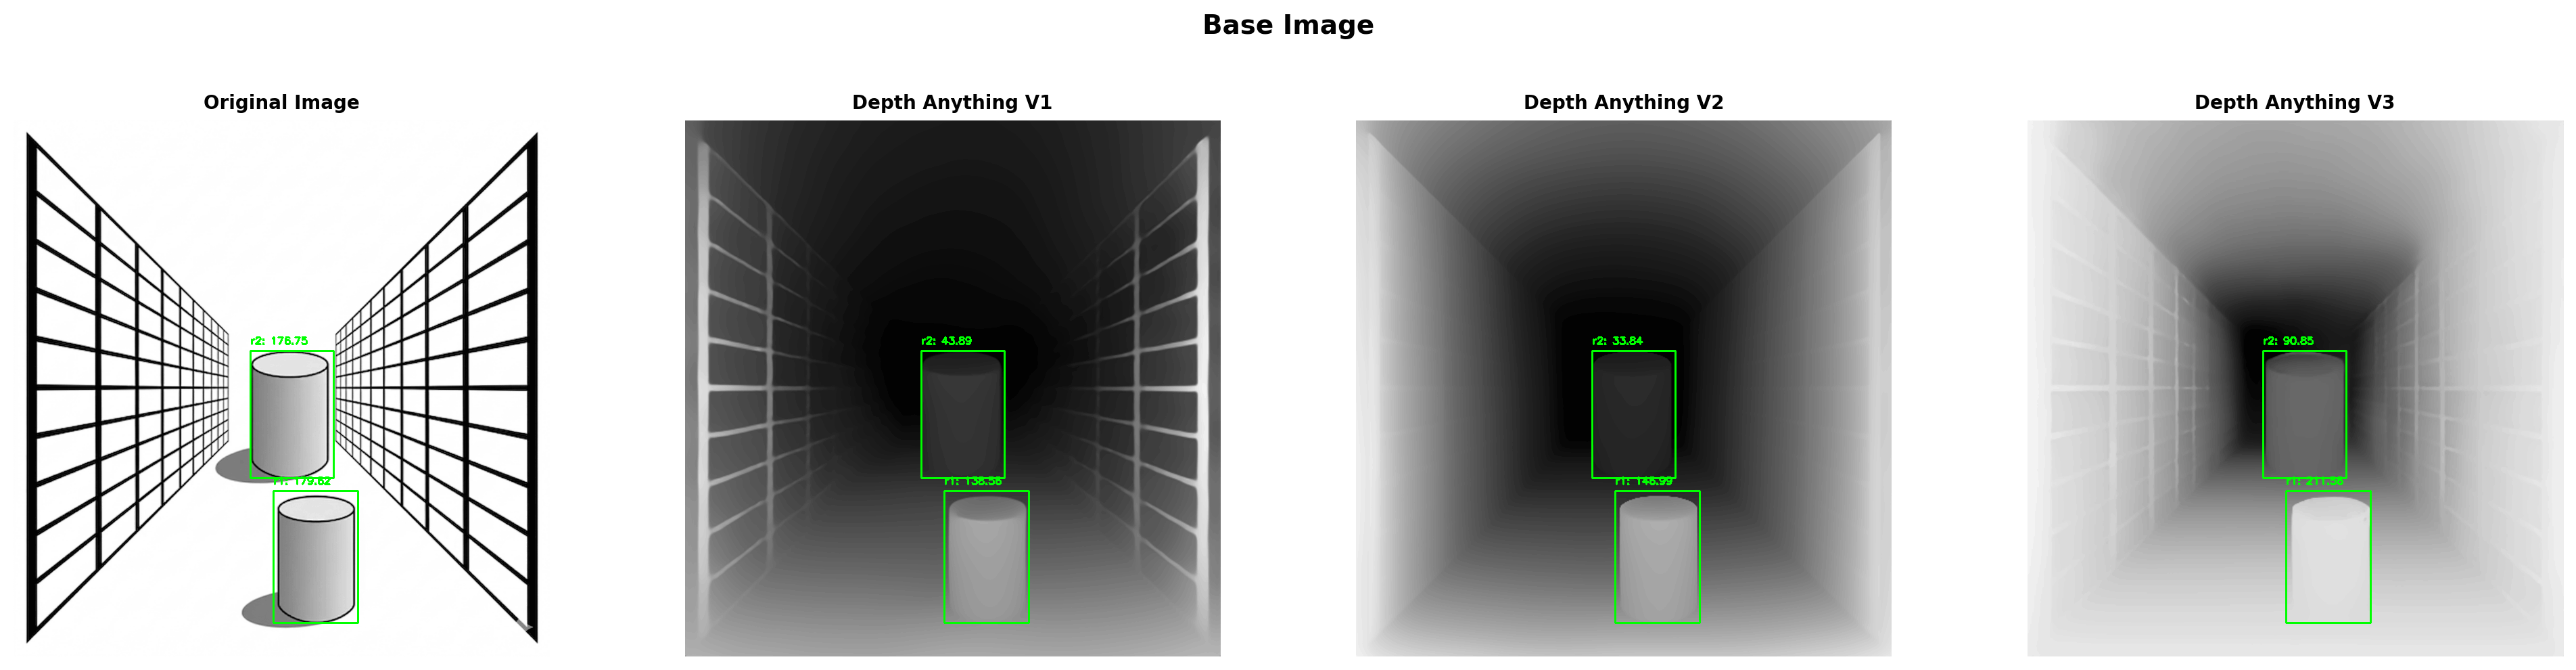
\includegraphics[width=\linewidth]{figures/fig_roi_example}
  \caption{ROI extraction for the Corridor Illusion. Two bounding boxes (A, B) are placed
           over the geometrically equidistant cylinders. The mean pixel intensity
           $I_{\text{mean}}$ is computed per region directly from the model's depth map
           output, and Eq.~\ref{eq:depthgap} converts the pair of region means into the
           single $\Delta I$ value reported throughout Section~\ref{sec:results}.}
  \label{fig:roi}
\end{figure}

\subsection{Synthetic Stimuli Engineering}

An ablation study over the Corridor Illusion isolates the visual features that trigger
depth perception. Fig.~\ref{fig:corridor} shows the baseline depth maps before any
ablation is applied. Fifteen controlled variants are generated across five sub-categories:
structural context/boundary ablation, shadow \& lighting logic, feature augmentation,
semantic \& geometric consistency, and frequency domain analysis.

\begin{figure}[H]
  \centering
  % Replace with actual figure
  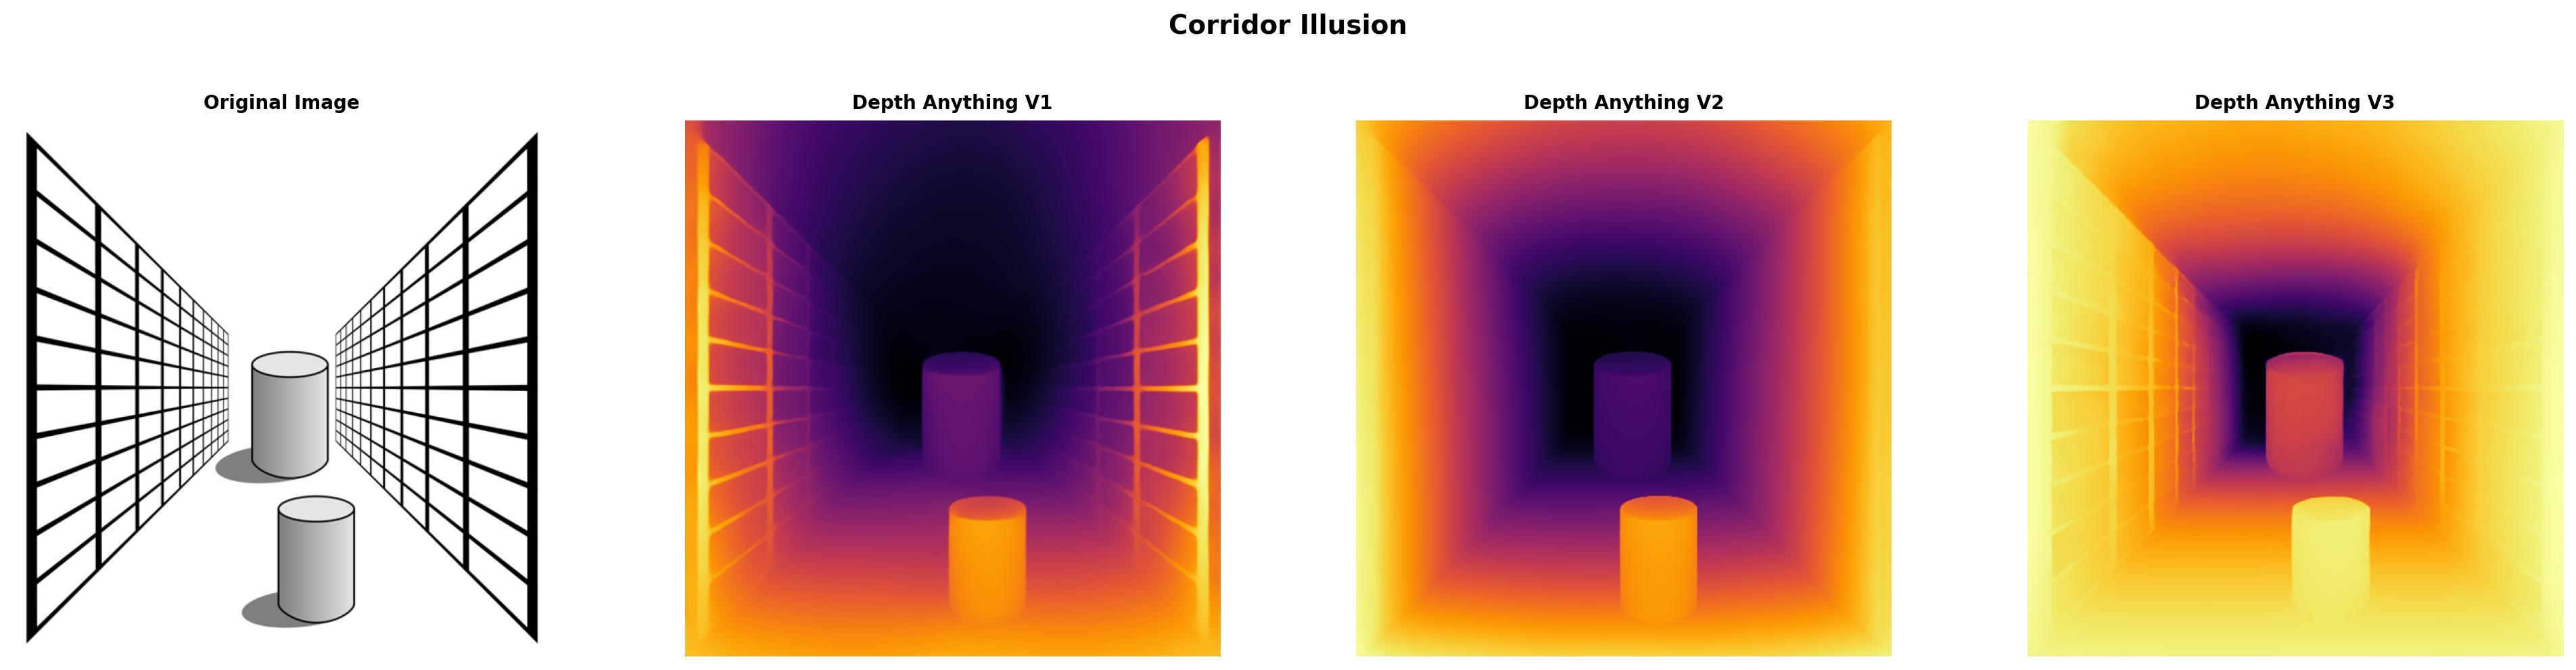
\includegraphics[width=\linewidth]{figures/fig_corridor_comparison}
  \caption{Depth maps of the Corridor Illusion (V1, V2, V3). Brighter = closer.
           All models assign greater depth to the geometrically higher cylinder.}
  \label{fig:corridor}
\end{figure}

\subsection{Artificial Psychophysics Framework}

Inspired by classical psychophysics~\cite{gescheider1997}, each VFM is treated as a
\emph{perceptual agent}. It is important to note that this framework does not imply
conscious perception or any phenomenological experience on the part of the model;
classical psychophysical terminology such as PSE and JND is used here strictly in an
operational sense, as a standardised mathematical framework to characterise output
sensitivity and systematic bias under controlled, incremental visual perturbation.

Stimuli are presented as 30-frame sequences with a single
parameter varied incrementally (e.g.\ object height, line convergence angle, shadow
distance). Unlike human psychophysics, where subjects are susceptible to guessing and
fatigue in a Two-Alternative Forced Choice task, this framework uses a continuous
discrimination task instead: the average intensity values for the two ROIs are extracted
across all 30 frames. Since the models are deterministic and do not suffer fatigue,
boredom, or learning effects, a linear progression of constant stimuli is used to capture
the full range of the model's response, rather than an adaptive staircase procedure.

The resulting $\Delta I$ curve is modelled via linear interpolation to extract:

\begin{itemize}
  \item \textbf{PSE (Point of Subjective Equality):} The stimulus level at which
        $\Delta I \approx 0$, i.e.\ the model perceives both ROIs as equidistant.
  \item \textbf{JND (Just Noticeable Difference):} The distance from the PSE to the
        84\%-maximum threshold (equivalent to $1\sigma$ of a cumulative Gaussian),
        quantifying the model's sensitivity.
\end{itemize}

A low JND (steep curve) indicates high sensitivity; a high JND indicates robustness.

\subsection{Voxel-Based Cross-Domain Validation}

Key illusions are reconstructed in Minecraft~\cite{minecraft2011}, a voxel engine that
eliminates the organic textures and high-frequency noise found in natural images. This acts as a stress test for the models since the environment provides a discretized geometry, a distinct lighting model, and the absence of organic textures.

% ============================================================
\section{Results}
\label{sec:results}

All results follow the evaluation protocol defined in Section~\ref{sec:method}: depth maps
are produced in inference-only mode with fixed model weights, ROIs are selected once per
stimulus and reused across all model versions, and $\Delta I$ (Eq.~\ref{eq:depthgap}) is
the primary quantitative metric. For psychophysics experiments, each stimulus sequence
runs for 30 frames with a single parameter varied linearly; PSE and JND are extracted via
linear interpolation of the resulting $\Delta I$ curve.

\subsection{Qualitative Evaluation on Classical Illusions}

\textbf{Converging Lines.} All three Depth Anything versions consistently assign greater
depth (darker pixels) to the geometrically \emph{higher} object in the Corridor (Fig. \ref{fig:corridor}) and Ponzo
illusion (Fig. \ref{fig:ponzo_map}), mirroring the human tendency to interpret height-in-field as distance. V3
produces the sharpest depth boundaries but also the noisiest edges under complex
structure.

\textbf{Depth Ambiguity.} On Schröeder's Stairs, all models converge on the statistically
dominant interpretation (light from above) (See fig.~\ref{fig:schroeder_stairs_map}). V1 fails to produce a coherent Necker's Cube
interpretation; V2 partially separates the faces; V3 confidently commits to the standard
orientation (see Fig.~\ref{fig:necker}).

\begin{figure}[H]
  \centering
  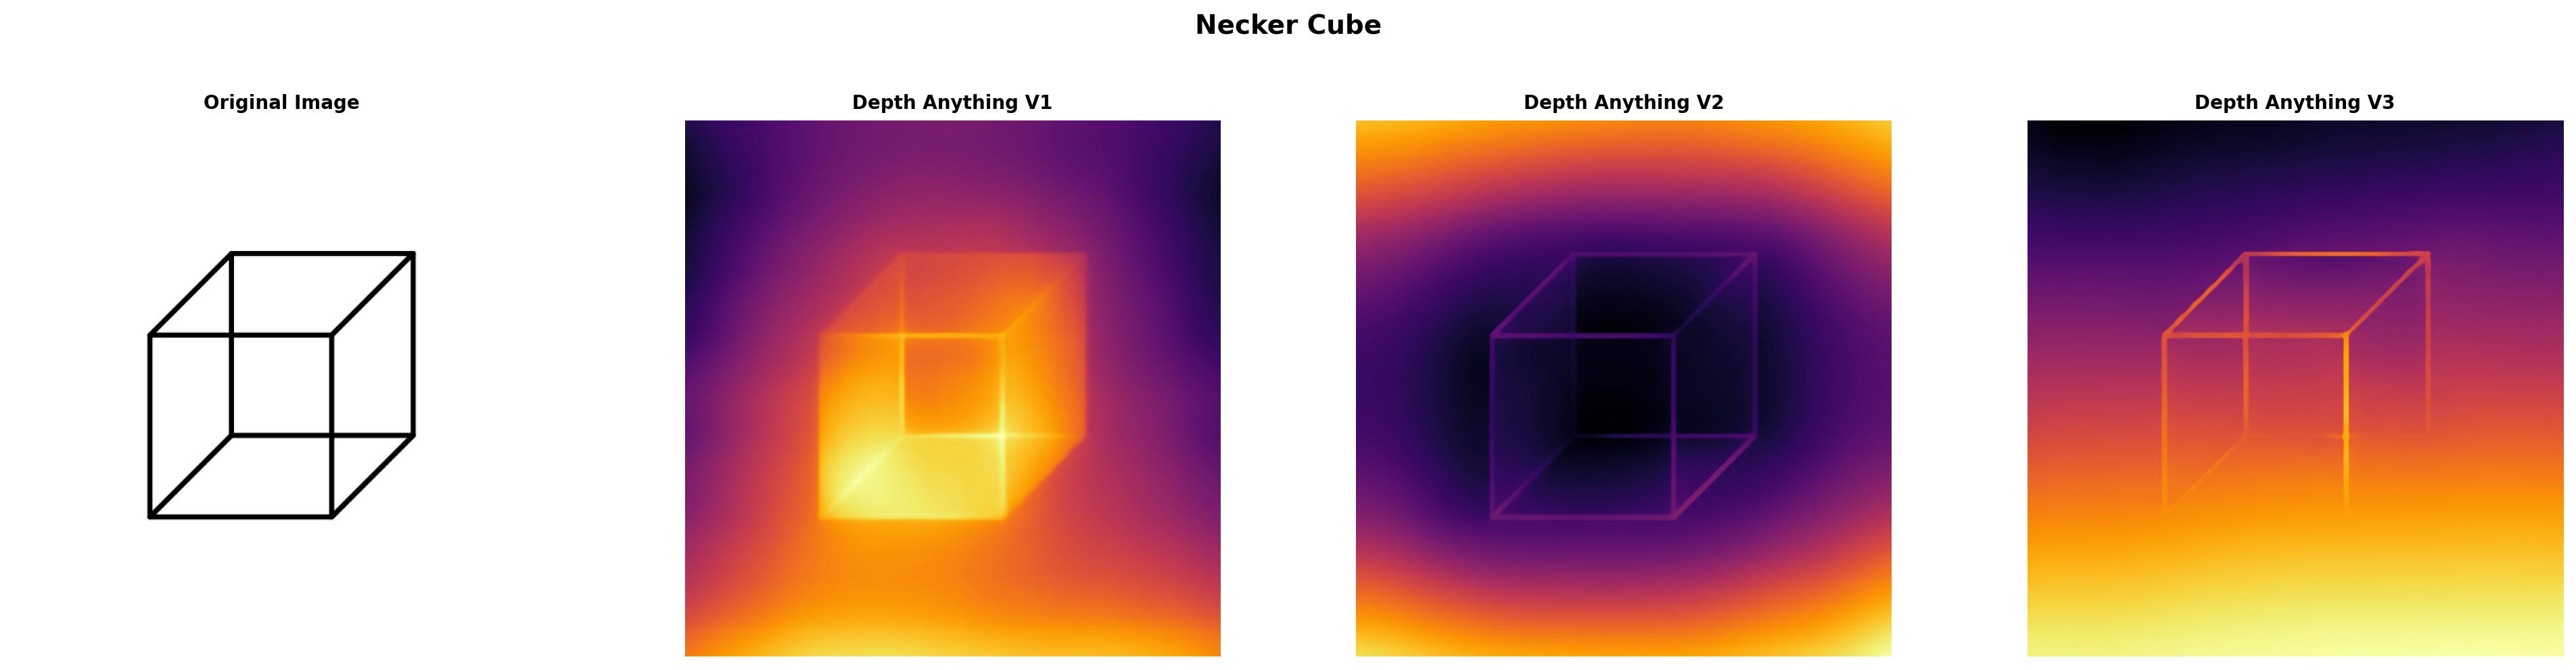
\includegraphics[width=\linewidth]{figures/fig_necker_cube}
  \caption{Necker Cube processed by V1, V2, and V3. The models show different ways of failing when faced with the ambiguous drawing. V1 treats the entire object as a single mass close to the camera, with no internal depth. V2 applies a strong centrality bias, interpreting the center of the image as being far away (like a hole). V3 does not perceive the 3D geometry at all and simply generates a top-to-bottom gradient (height-in-field), treating the structure as a flat 2D pattern.}
  \label{fig:necker}
\end{figure}

\textbf{Forced Perspective.} This category is where VFMs are most robust. On the Ames
Room (Fig. \ref{fig:forced_perspective_combined}) and Beuchet's Chair (Fig. \ref{fig:Beuchet}), all three versions correctly identify that geometrically separate
elements are at different depths. Notably, V3 fails on the Salar de Uyuni image, grouping
distant figures with a nearby person, suggesting that semantic context can override
geometric reasoning (Fig.~\ref{fig:forced_perspective_combined}).

\begin{figure}[htbp]
  \centering
  % Cambia "forced_perspective_experiments" por el nombre exacto de tu archivo único
  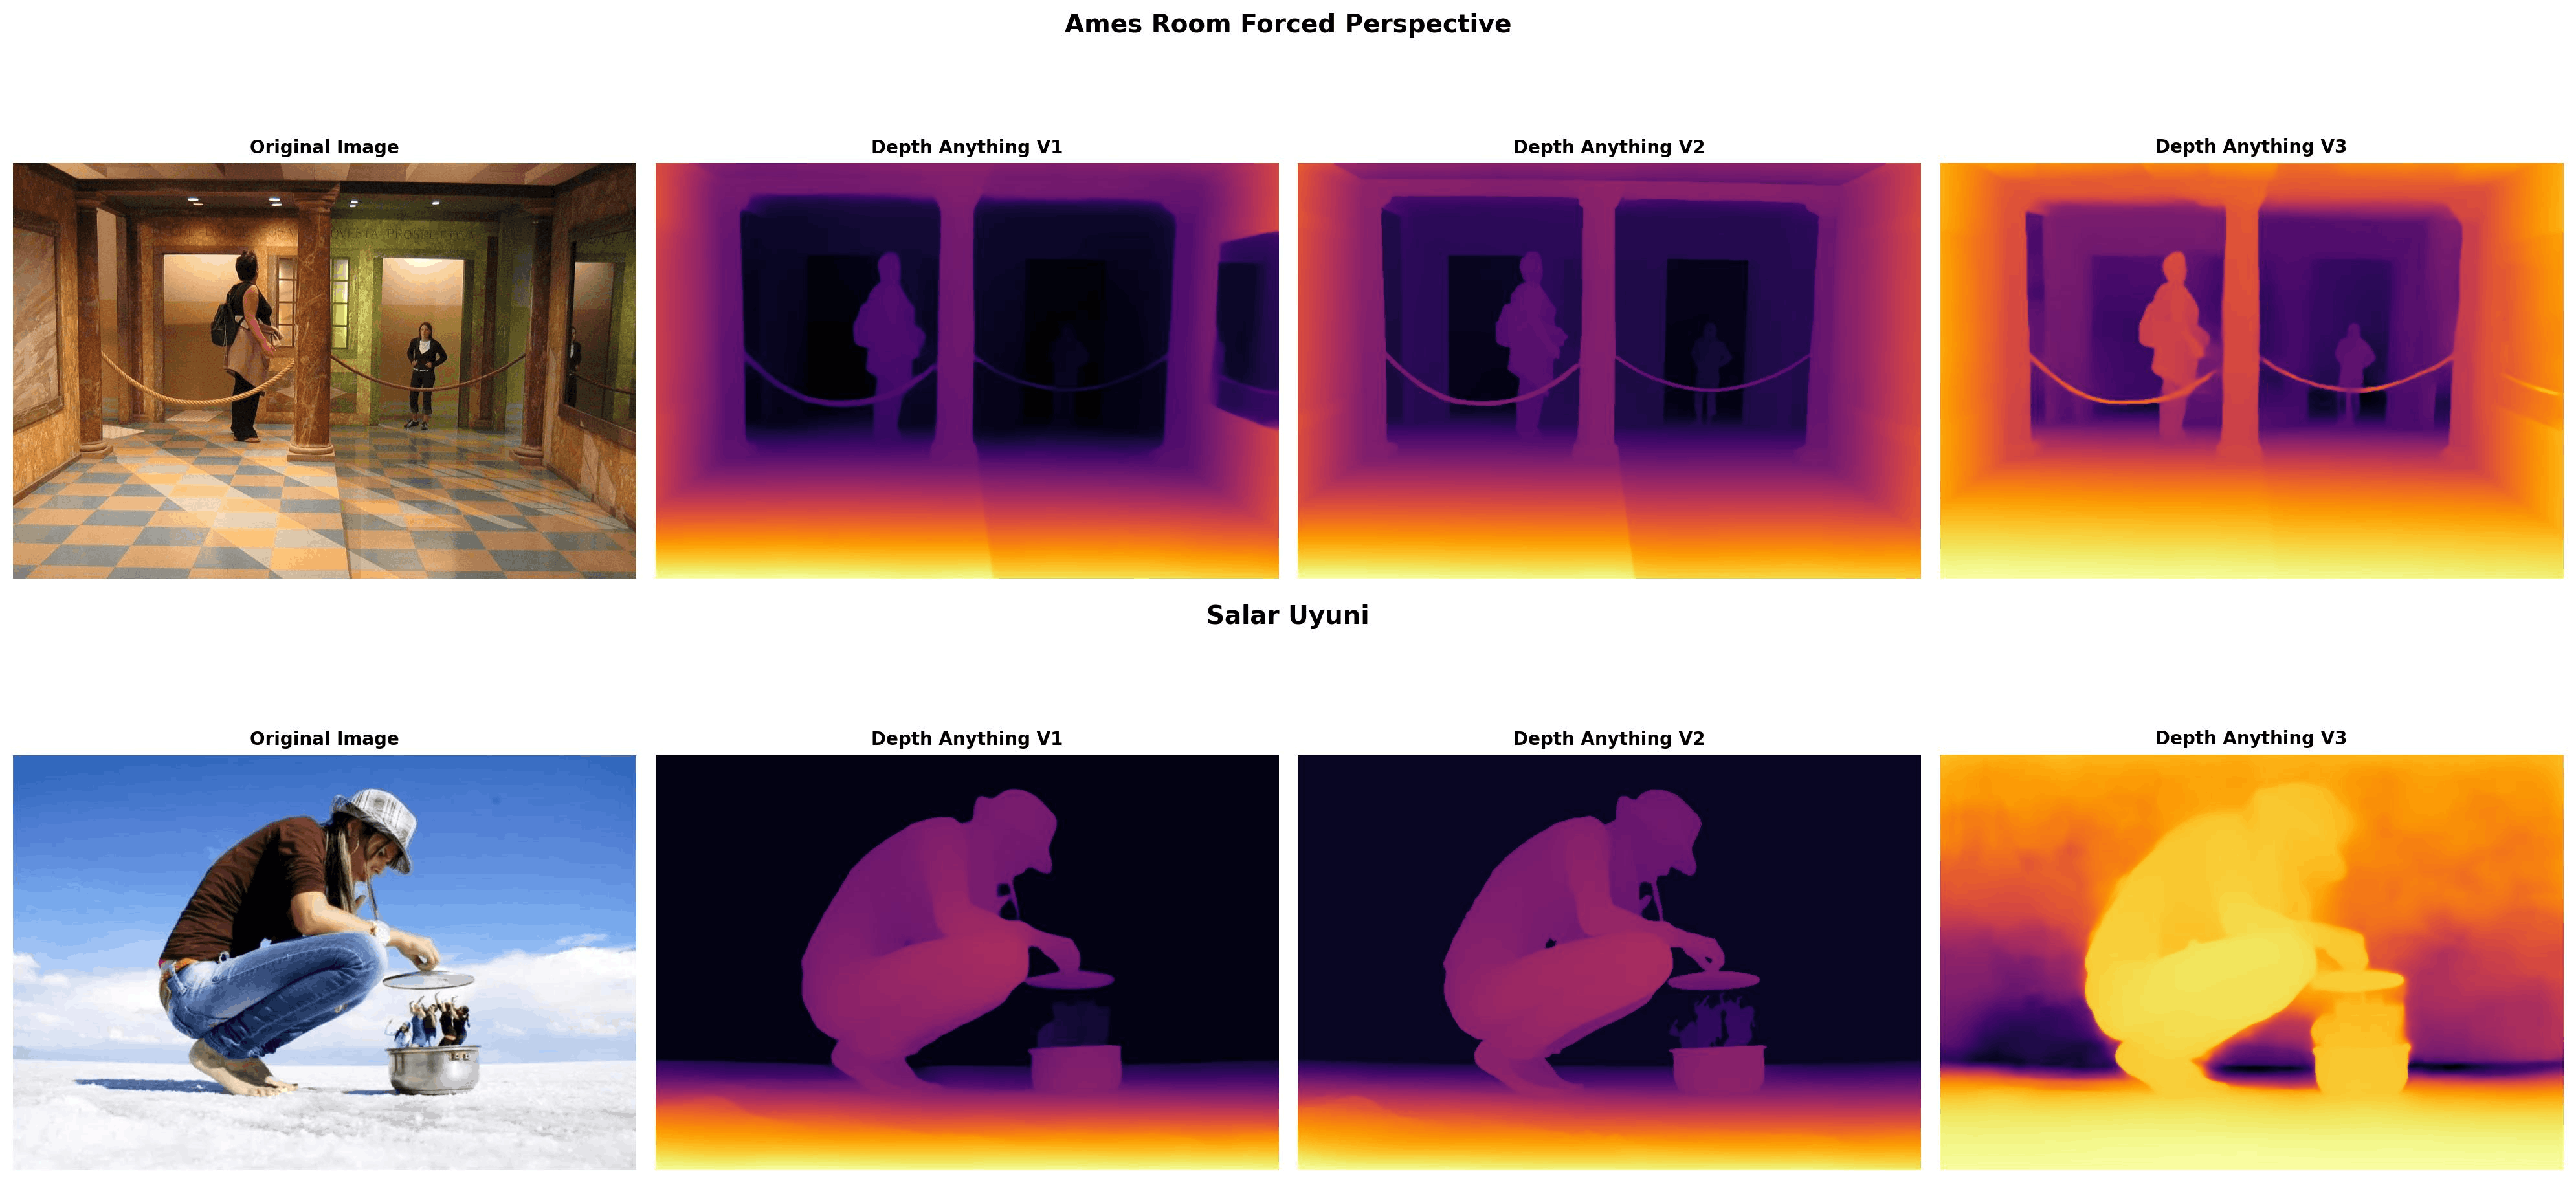
\includegraphics[width=\linewidth]{figures/fig_ames_uyuni.png}
  \caption{Forced perspective experiments. Top: Ames Room illusion, where all three models successfully resolve the true physical depth of the subjects despite the geometric distortion. Bottom: Salar de Uyuni experiment, where V1 and V2 correctly isolate the distant background figures, but V3 fails completely by putting them at the exact same depth level as the foreground woman.}
  \label{fig:forced_perspective_combined}
\end{figure}

\textbf{Impossible Objects.} V1 and V2 preserve local coherence while generating globally
inconsistent depth gradients. V3 produces high-contrast artifacts at topologically
impossible junctions. It attempts global coherence and fails visibly when none is possible
(see Fig.~\ref{fig:eschercube}).

\begin{figure}[H]
  \centering
  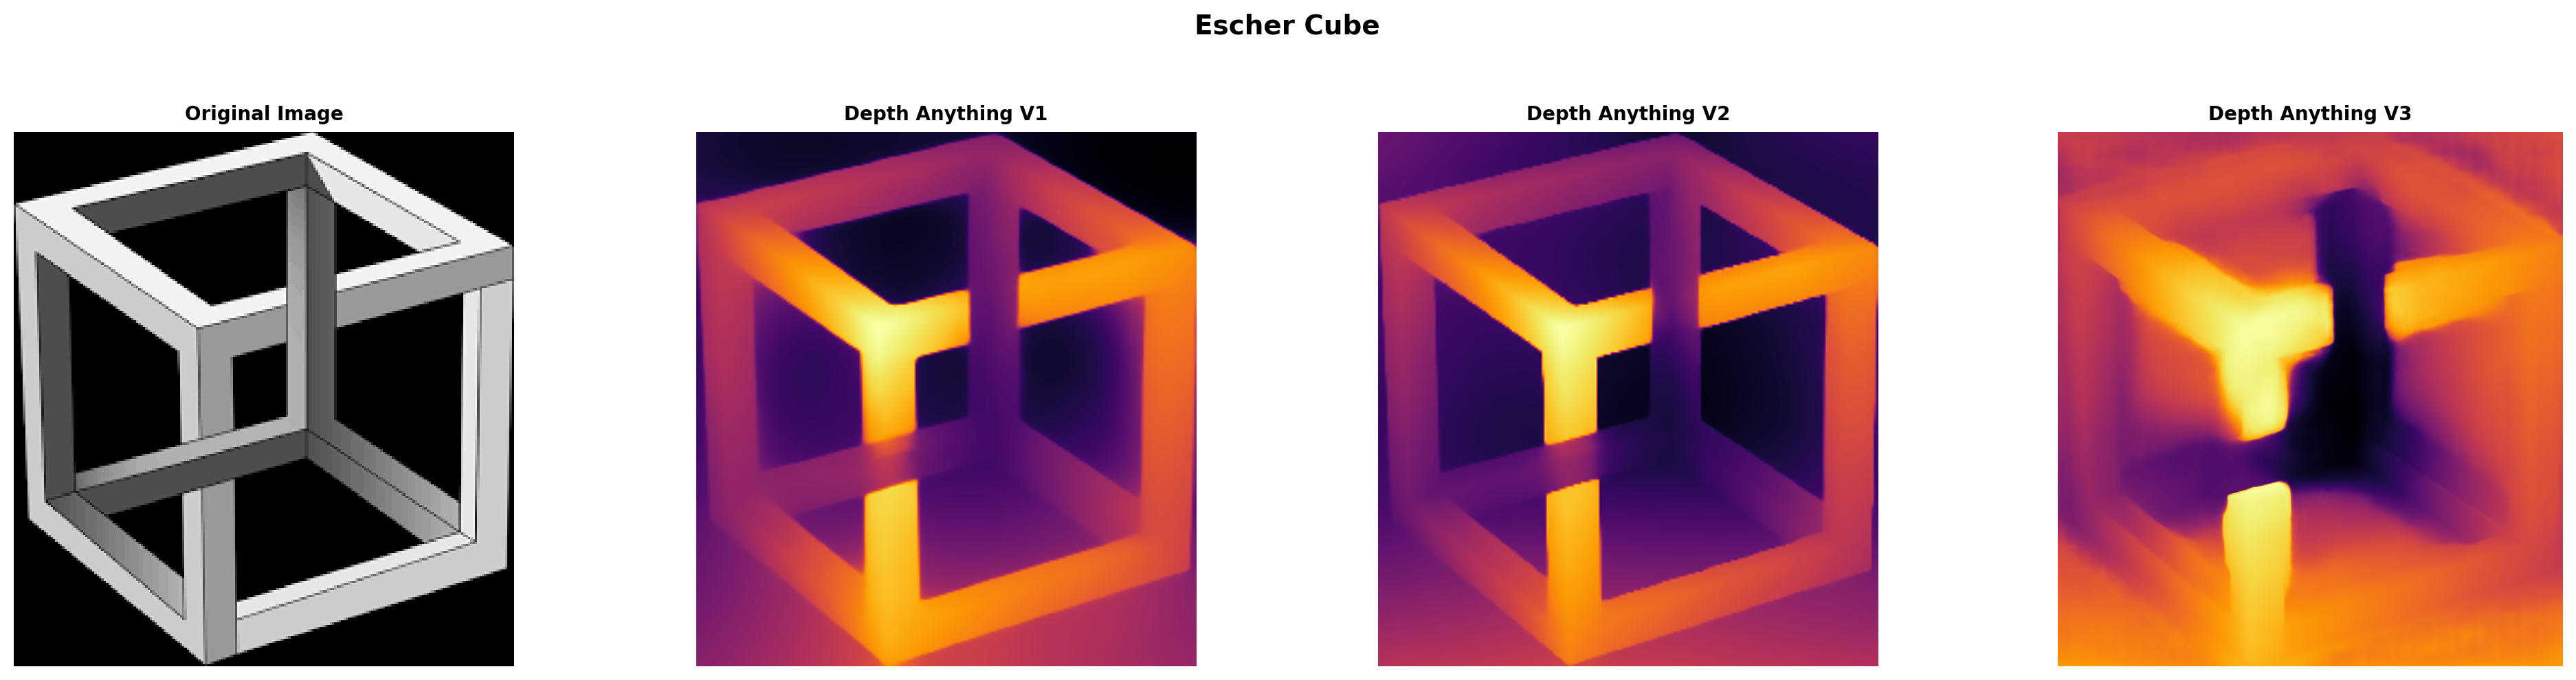
\includegraphics[width=\linewidth]{figures/fig_escher_cube}
  \caption{Escher's Cube processed by V1, V2 and V3. V1 and V2 resolve the impossible
           intersection by fusing the overlapping faces; V3 instead fractures the structure
           and produces sharp, high-contrast artifacts at the contradictory junction.}
  \label{fig:eschercube}
\end{figure}

\textbf{Shading \& Illumination.} All three models replicate the hollow-face prior
(perceiving concave faces as convex), with V3 showing the highest $\Delta I$. The
Gardner's Dragon confirms a strong shape-from-shading bias across all versions
(Fig.~\ref{fig:gardner_dragon}).

\begin{figure}[htbp]
  \centering
  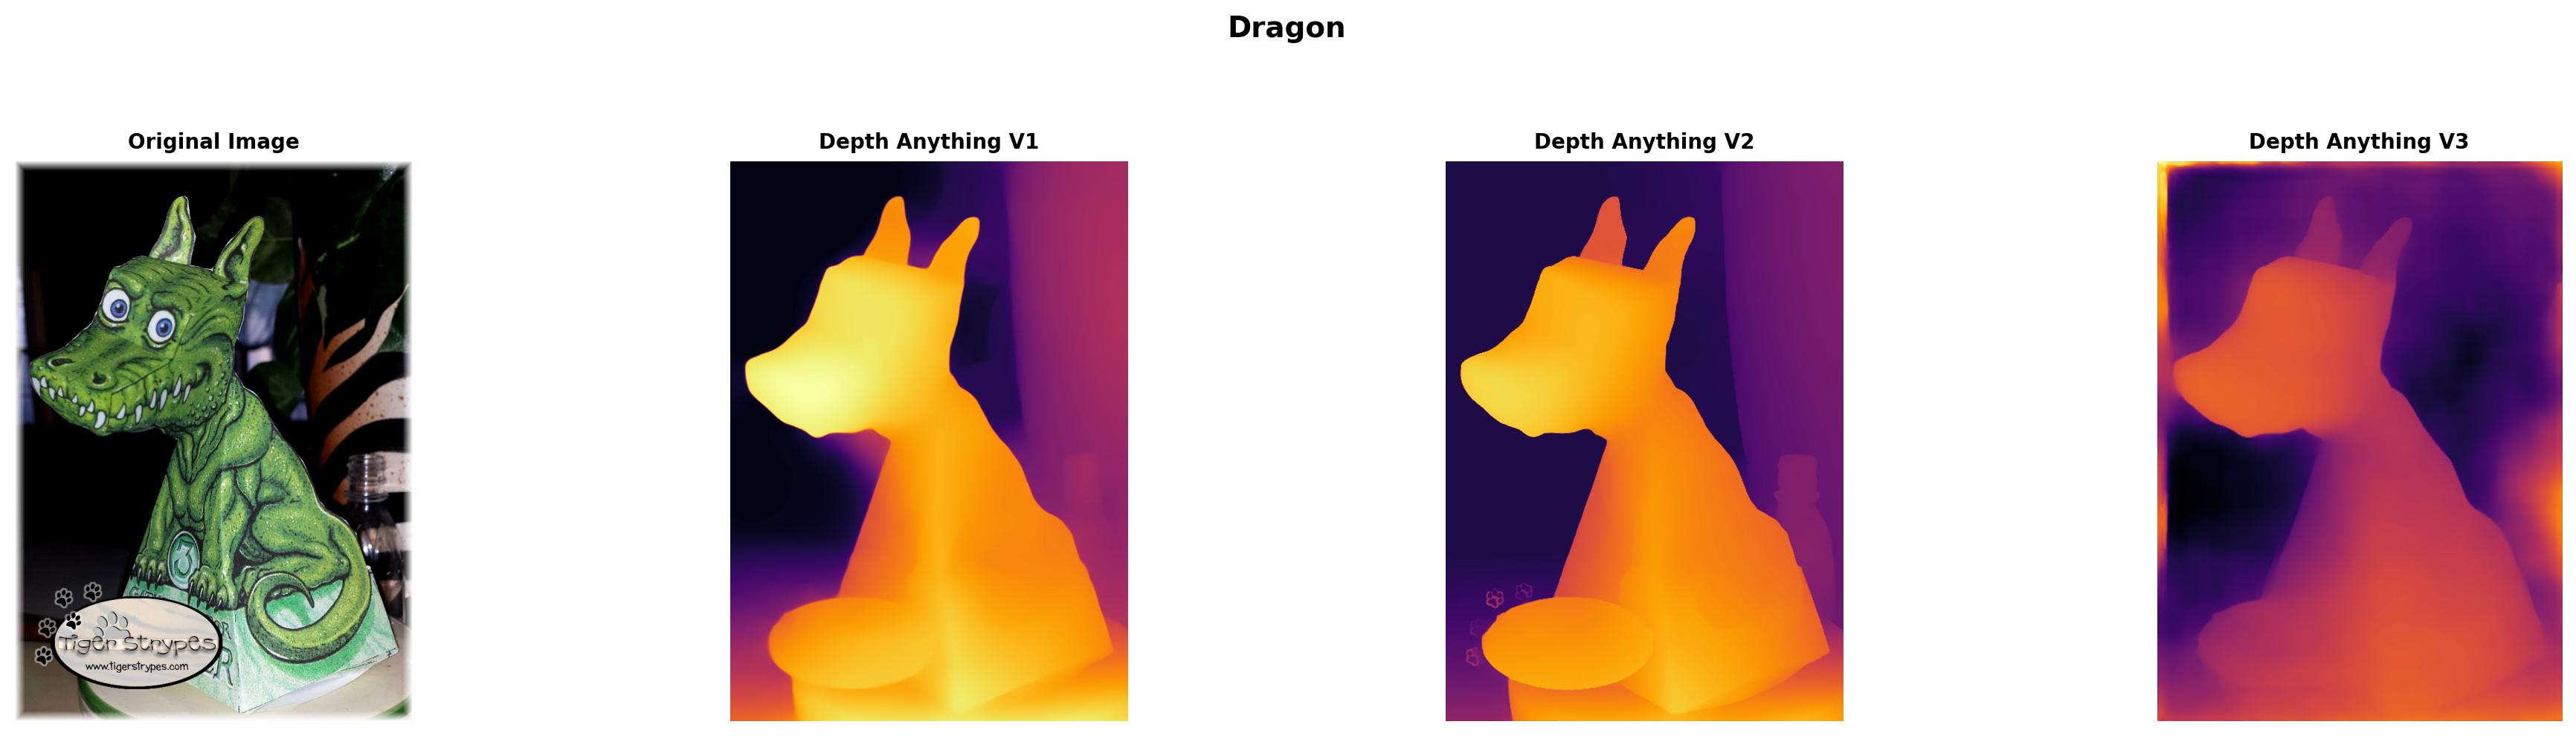
\includegraphics[width=\linewidth]{figures/fig_gardner_dragon.jpg}
  \caption{Gardner's Dragon illusion.  all three Depth Anything models interpret the concave 2D face as a 3D convex volume. The models incorrectly assign the highest proximity (bright yellow pixels) to the dragon's snout, confirming a strong shape-from-shading bias.}
  \label{fig:gardner_dragon}
\end{figure}

\subsection{Synthetic Stimuli Engineering}

Table~\ref{tab:corridor} summarizes the illusory depth gap $\Delta I$ across all 15
corridor variants; some of them are shown in Fig.~\ref{fig:fig_synth_data}. 
\begin{table*}[t]
\centering
\caption{Illusory depth gap ($\Delta I$) across the fifteen Corridor Illusion variants for
all four models.  The stronger the value, the stronger the intensity perceived.}
\label{tab:corridor}
\small
\setlength{\tabcolsep}{0pt} % Elimina espacios extra entre columnas
\begin{tabular*}{\textwidth}{@{\extracolsep{\fill}}llccccl@{}} % \textwidth asegura que ocupe todo el ancho
\toprule
\textbf{Experiment} & \textbf{Category} & \textbf{V1 $\Delta I$} & \textbf{V2 $\Delta I$} & \textbf{V3 $\Delta I$} & \textbf{MiDaS $\Delta I$} & \textbf{Notes} \\
\midrule
Base Corridor        & Structural   & 94.7  & 113.2 & 120.7 & 108.4 & Baseline \\
No Walls             & Structural   & 125.1 & 120.8 &  43.0 &  98.9 & V3 drops 65\%; MiDaS barely affected \\
Cube Walls           & Structural   & 145.5 & 143.8 &  47.9 & 152.1 & V1/V2/MiDaS increase; V3 reads as enclosed space \\
Warped Corridor      & Structural   &  97.4 &  78.4 &  91.8 &  47.8 & MiDaS shows the largest drop \\
Solid (no shadow)    & Lighting     &  68.2 &  89.2 &  77.8 &  64.9 & Shadow removal reduces all models \\
Solid Bordered       & Lighting     &  74.3 &  86.5 & 147.7 &  66.9 & V3 spikes; MiDaS stays close to base \\
Cylinder Pattern     & Augmentation &  89.3 &  90.4 & 127.0 &  82.6 & Texture distracts V1/V2; boosts V3 \\
Pattern Bordered     & Augmentation &  91.6 & 100.4 & 122.6 &  88.4 & Consistent with pattern \\
No Cylinders & Semantic     &  92.9 &  94.5 & 120.0 &  53.9 & Semantics irrelevant for V1/V2/V3 \\
Only Cylinders       & Semantic     &  65.5 &  11.9 &   6.4 &  71.4 & Context removal breaks V2/V3, not MiDaS \\
Size Prior           & Semantic     &  95.4 & 111.5 & 126.6 & 107.2 & Large object does not override position \\
Shepard Illusion     & Semantic     &  27.2 &  17.8 &  24.0 & 139.6 & Horizontal orientation weakens V1/V2/V3 \\
Low-pass             & Frequency    & 119.2 & 126.7 &  65.4 &  93.7 & V1/V2 fully triggered by low-freq \\
High-pass            & Frequency    & 110.5 & 103.0 &  89.3 &  75.5 & High-freq edges sufficient for V1/V2 \\
High-low filter      & Frequency    &  72.3 &  85.5 &  13.6 &  77.2 & V3 collapses; MiDaS does not \\
\midrule
Minecraft Corridor   & Cross-domain &  23.3 &  29.1 & 118.4 &  30.9 & V3 transfers strongly \\
\bottomrule
\end{tabular*}
\end{table*}

Key findings from the ablation:
\begin{itemize}
  \item \textbf{V1 and V2} maintain high $\Delta I$ even under heavy context removal,
        indicating primitive, hard-coded priors (height-in-field and centrality, respectively).
  \item \textbf{V3} is highly context-dependent: it achieves the highest $\Delta I$ when
        full cues are present, but collapses near zero when structural cues are removed
        (``Only Cylinders'': $\Delta I = 6.4$; High-low filter: $\Delta I = 13.6$).
  \item \textbf{MiDaS} is the most context-independent of the four models. ``Only
        Cylinders'' barely changes its $\Delta I$ (71.4, close to the base value), and even
        the high-low frequency split, which collapses V3 to 13.6, keeps MiDaS at 77.2.
        Its prior is also indifferent to object orientation: the Shepard Illusion, which
        weakens the bias for V1, V2 and V3, produces the single highest $\Delta I$ recorded
        for MiDaS in this table (139.6).
\end{itemize}

\begin{figure}[htbp]
  \centering
  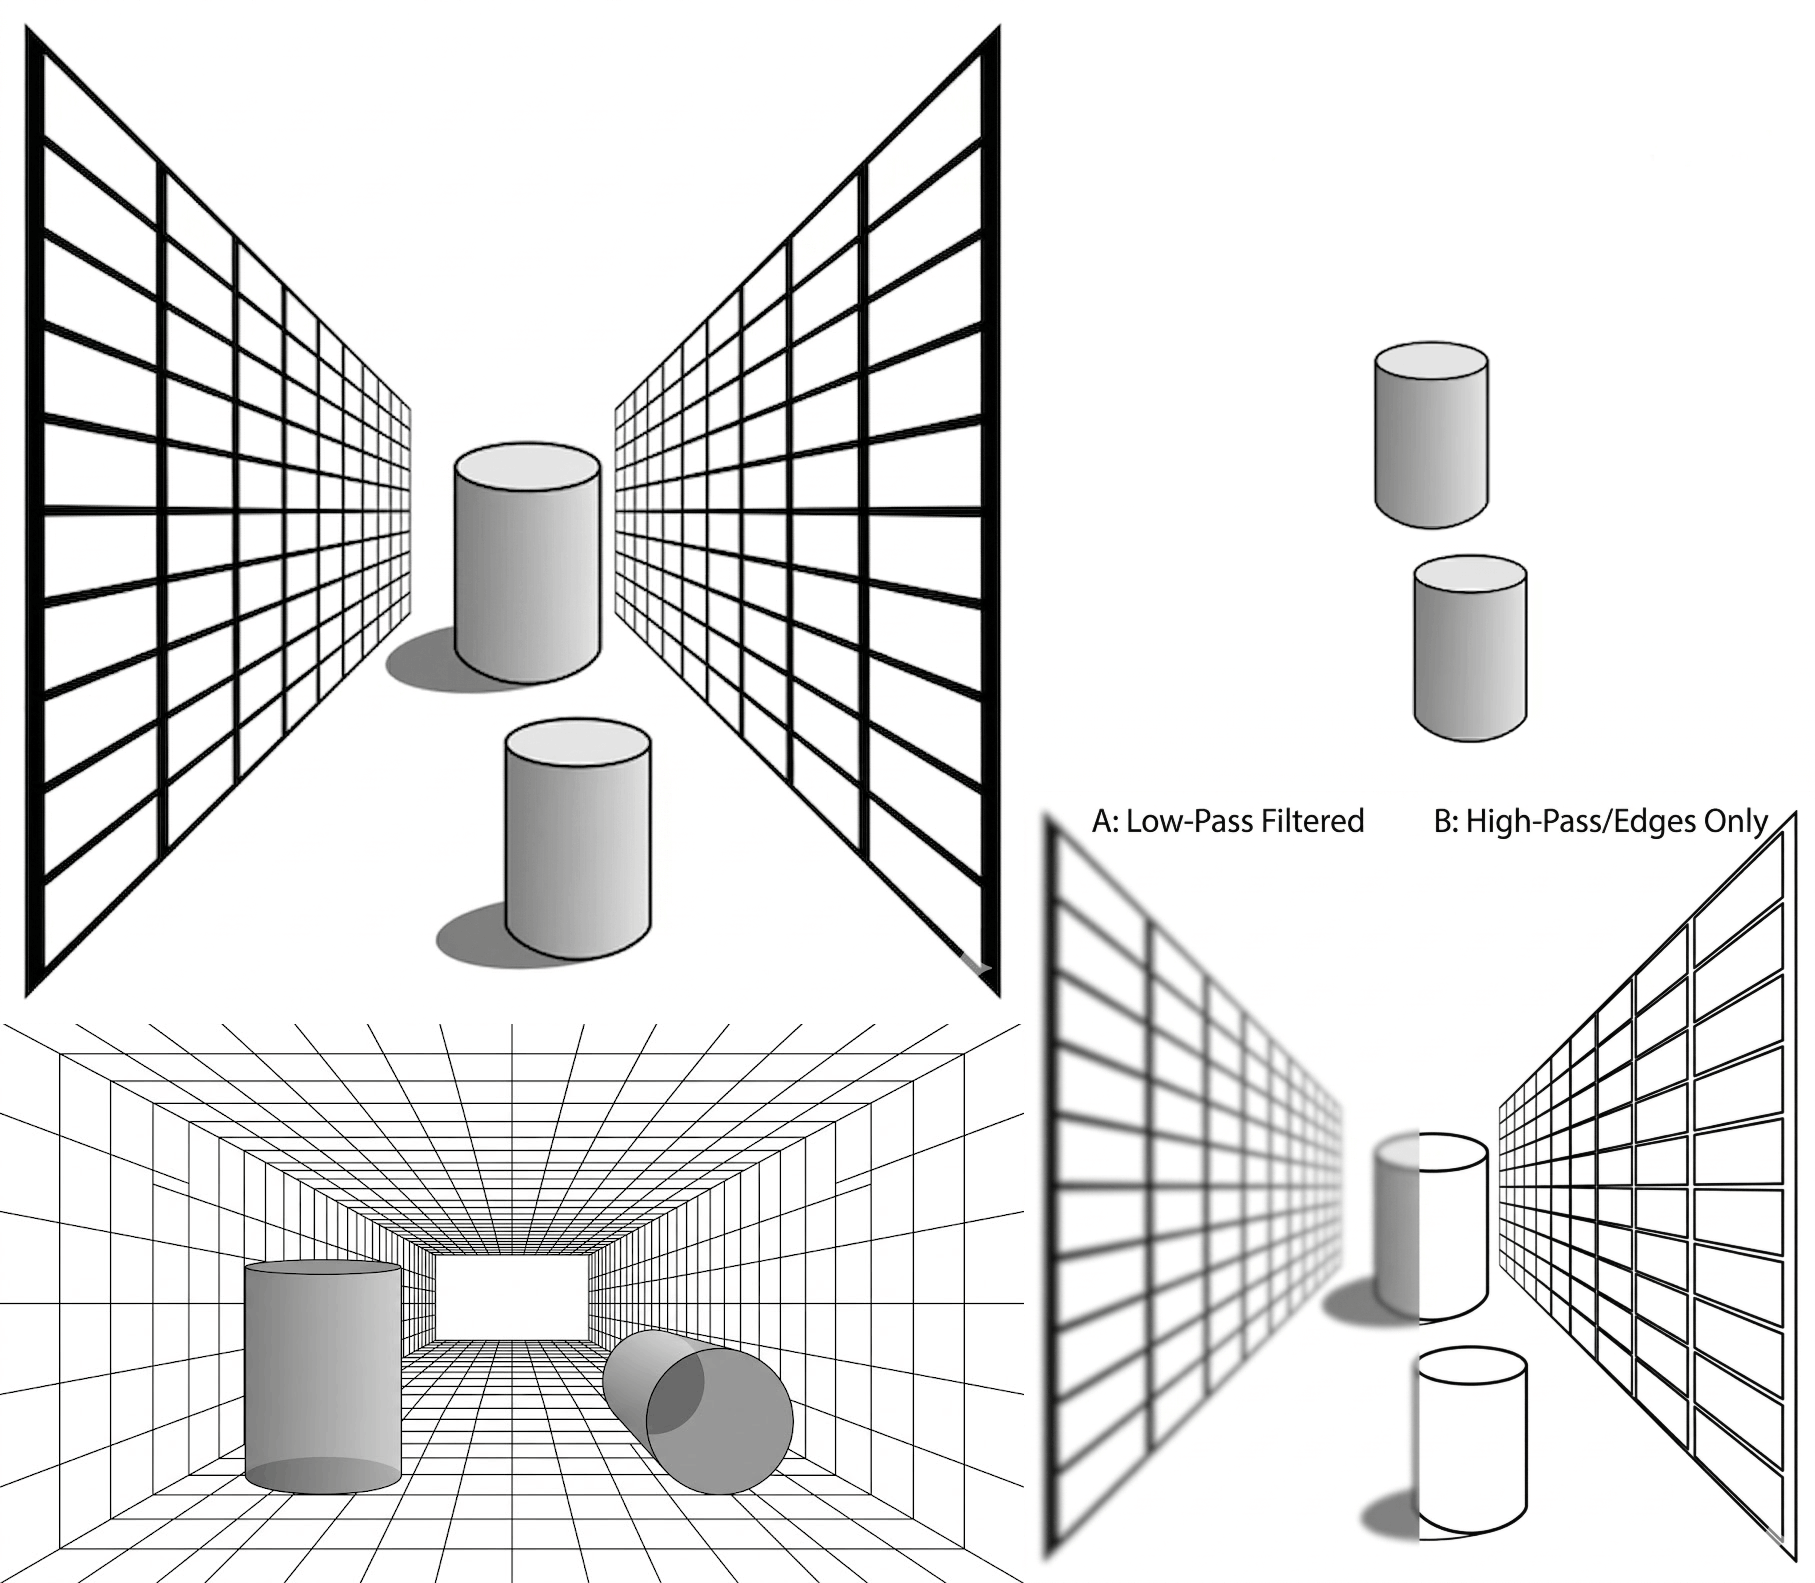
\includegraphics[width=\linewidth]{figures/fig_synth_data}
  \caption{Key stimuli from the Corridor Illusion ablation study. Top-left: Base Corridor, the original image. Top-right: Only Cylinders, to test content removal. Bottom-left: Shepard Illusion, altering the structural and semantic orientation. Bottom-right: High-low frequency filter, separating visual domains.}
  \label{fig:fig_synth_data}
\end{figure}
\subsection{Image-to-3D Generative Pipelines}

To extend the analysis beyond flat depth maps, Hunyuan3D 2.1~\cite{hunyuan3d} was
integrated into the workflow and used as an auxiliary interpretation engine to probe if the biases found in MDE models persist in Image-to-3D generative pipelines. A key advantage of this volumetric approach is that it removes the
ambiguity inherent to a 2D depth map: the resulting \texttt{.obj} mesh is an unequivocal
representation of how the model has interpreted the scene's geometry, with no room for
a different reading of the same grayscale image.

This is particularly informative for the impossible objects category, where a mesh
generator cannot represent a topological contradiction and is forced to choose one of
two resolutions. Escher's Cube and Escher's Waterfall are both resolved by the generator
through some form of hallucination: depending on the object, faces are merged together
to remove the impossibility, or the structure is broken apart into disconnected fragments
that no longer form a single coherent shape (Fig.~\ref{fig:3d_reconstruction}). The hollow-face prior identified in the 2D depth maps is observed to persist in this 3D setting; the model consistently reconstructs both the convex face and the concave mask as bulging outward in the same direction, providing clear qualitative evidence of the strength of this convexity prior (Fig.~\ref{fig:hollow_face_3d}). The Anamorphic Hole street art, a flat painting designed to look
like a hole in the ground from one specific viewpoint, is reconstructed by the model as
an actual three-dimensional hole, showing full susceptibility to the forced-perspective
trick even when the output is a literal 3D object rather than a 2D estimate.

Despite this analytical clarity, the generative pipeline is used here only as an auxiliary exploration rather than as the primary metric for spatial reasoning. While Hunyuan3D 2.1
produces good results when reconstructing isolated, individual objects, reconstruction
quality degrades noticeably once the input contains a more complex object or an entire
scene with multiple elements, which is a known limitation of current image-to-3D
pipelines rather than something specific to illusion stimuli. For this reason, the bulk of
the quantitative analysis in this work continues to rely on depth map estimation and the
$\Delta I$ metric defined in Section~\ref{sec:method}.

\begin{figure}[H]
  \centering
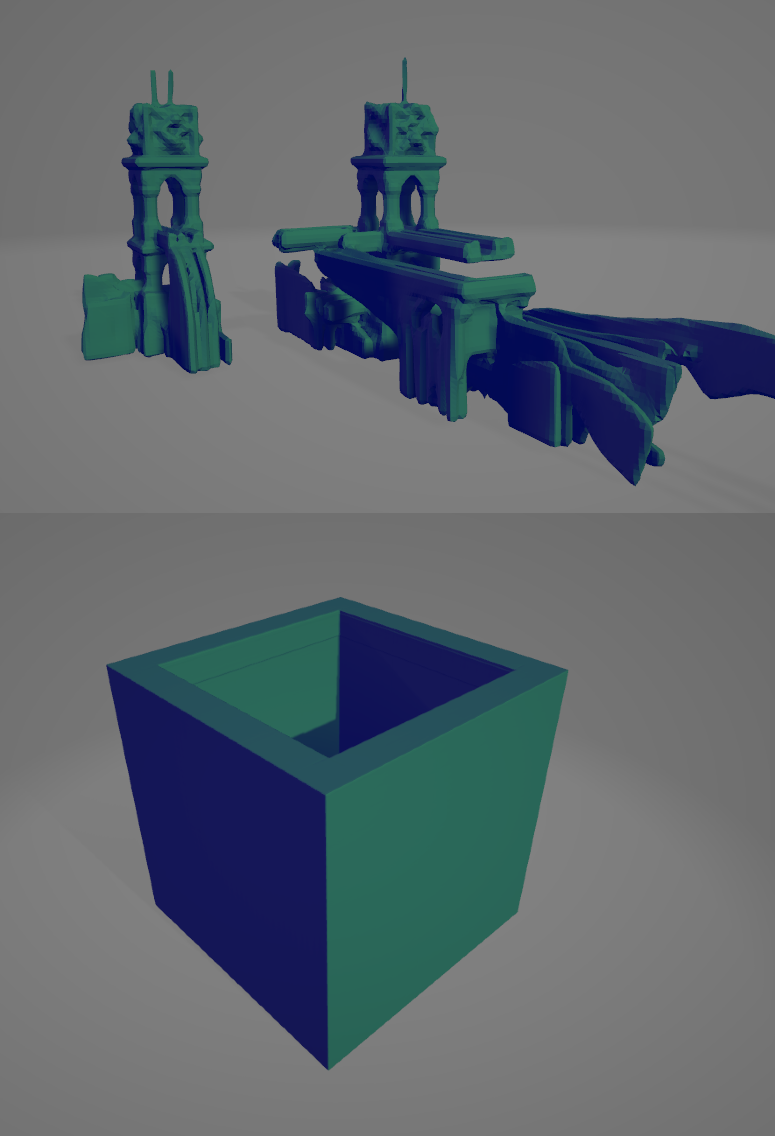
\includegraphics[height=0.2\textheight]{figures/fig_3d_reconstruction}
  \caption{Explicit 3D meshes generated by Hunyuan3D 2.1. Top: Escher's Waterfall; Bottom: Escher's Cube. Impossible objects are resolved through structural hallucination, where faces are either merged or fragmented to eliminate topological contradictions. Spatial biases are further confirmed by reconstructing the hollow-face illusion and anamorphic street art as physical 3D volumes.}
  \label{fig:3d_reconstruction}
\end{figure}

\begin{figure}[htbp]
  \centering
  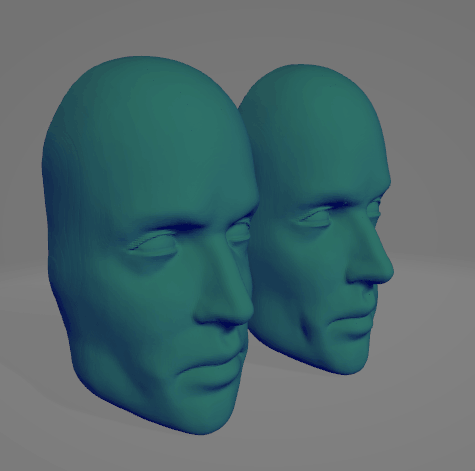
\includegraphics[width=0.4\linewidth]{figures/fig_hollow_face_mesh}
  \caption{Hollow Face illusion reconstructed as a 3D mesh by Hunyuan3D 2.1. Although the original 2D stimulus contains one convex face and one concave mask, the generative pipeline forces both to bulge outward in the same direction. This confirms the strong shape-from-shading bias and the hard-coded prior that faces must be convex.}
  \label{fig:hollow_face_3d}
\end{figure}

\subsection{Cross-Domain Validation: Voxel Laboratory}

In the voxel domain, spatial reasoning is broadly preserved despite the domain gap,
demonstrating that the identified priors are \emph{structural rather than texture-dependent}.

\textbf{Linear Perspective.} The converging tunnel produces $\Delta I$ values from 26
(V1) to 73 (V3), showing that vanishing-point structure alone is sufficient to trigger depth
biases. The flat-grid experiment confirms this: V1/V2 still predict depth from a horizontal
pattern, while V3 largely resists ($\Delta I \approx 7$).

\textbf{Depth Ambiguity.} Schröeder's Stairs (Fig.~\ref{fig:minecraftstairs}) in voxels confirm the light-from-above prior.
The rotated version flips the sign of $\Delta I$ for V1/V2 ($+17 \rightarrow -25$), while V3
maintains a positive value (+10), suggesting an alternative structural anchor.

\textbf{Shading \& Illumination.} Smooth lighting (no hard shadows) causes V3's corridor
confidence to spike from 81 to 127, confirming strong shadow-attachment sensitivity.
Fig.~\ref{fig:minecraft} shows the voxel corridor that underlies this experiment,
processed by V1, V2 and V3.

\begin{figure}[H]
  \centering
  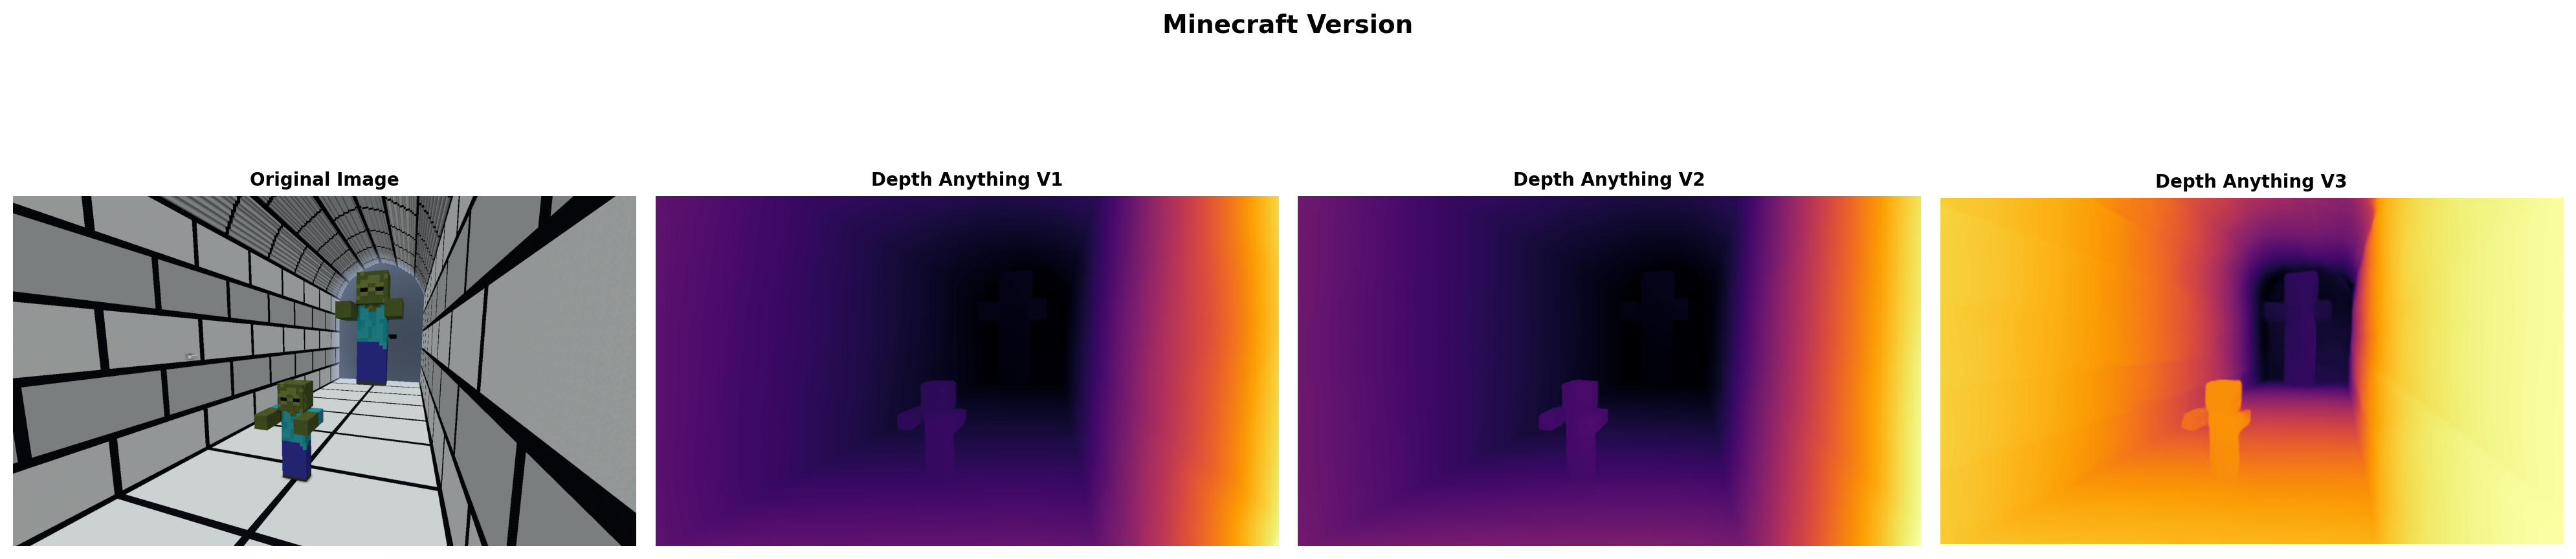
\includegraphics[width=\linewidth]{figures/fig_minecraft_corridor}
  \caption{Voxel corridor (Minecraft) processed by V1, V2, V3. Despite discrete block
           boundaries and absent textures, depth biases persist.}
  \label{fig:minecraft}
\end{figure}
\begin{figure}[H]
  \centering
  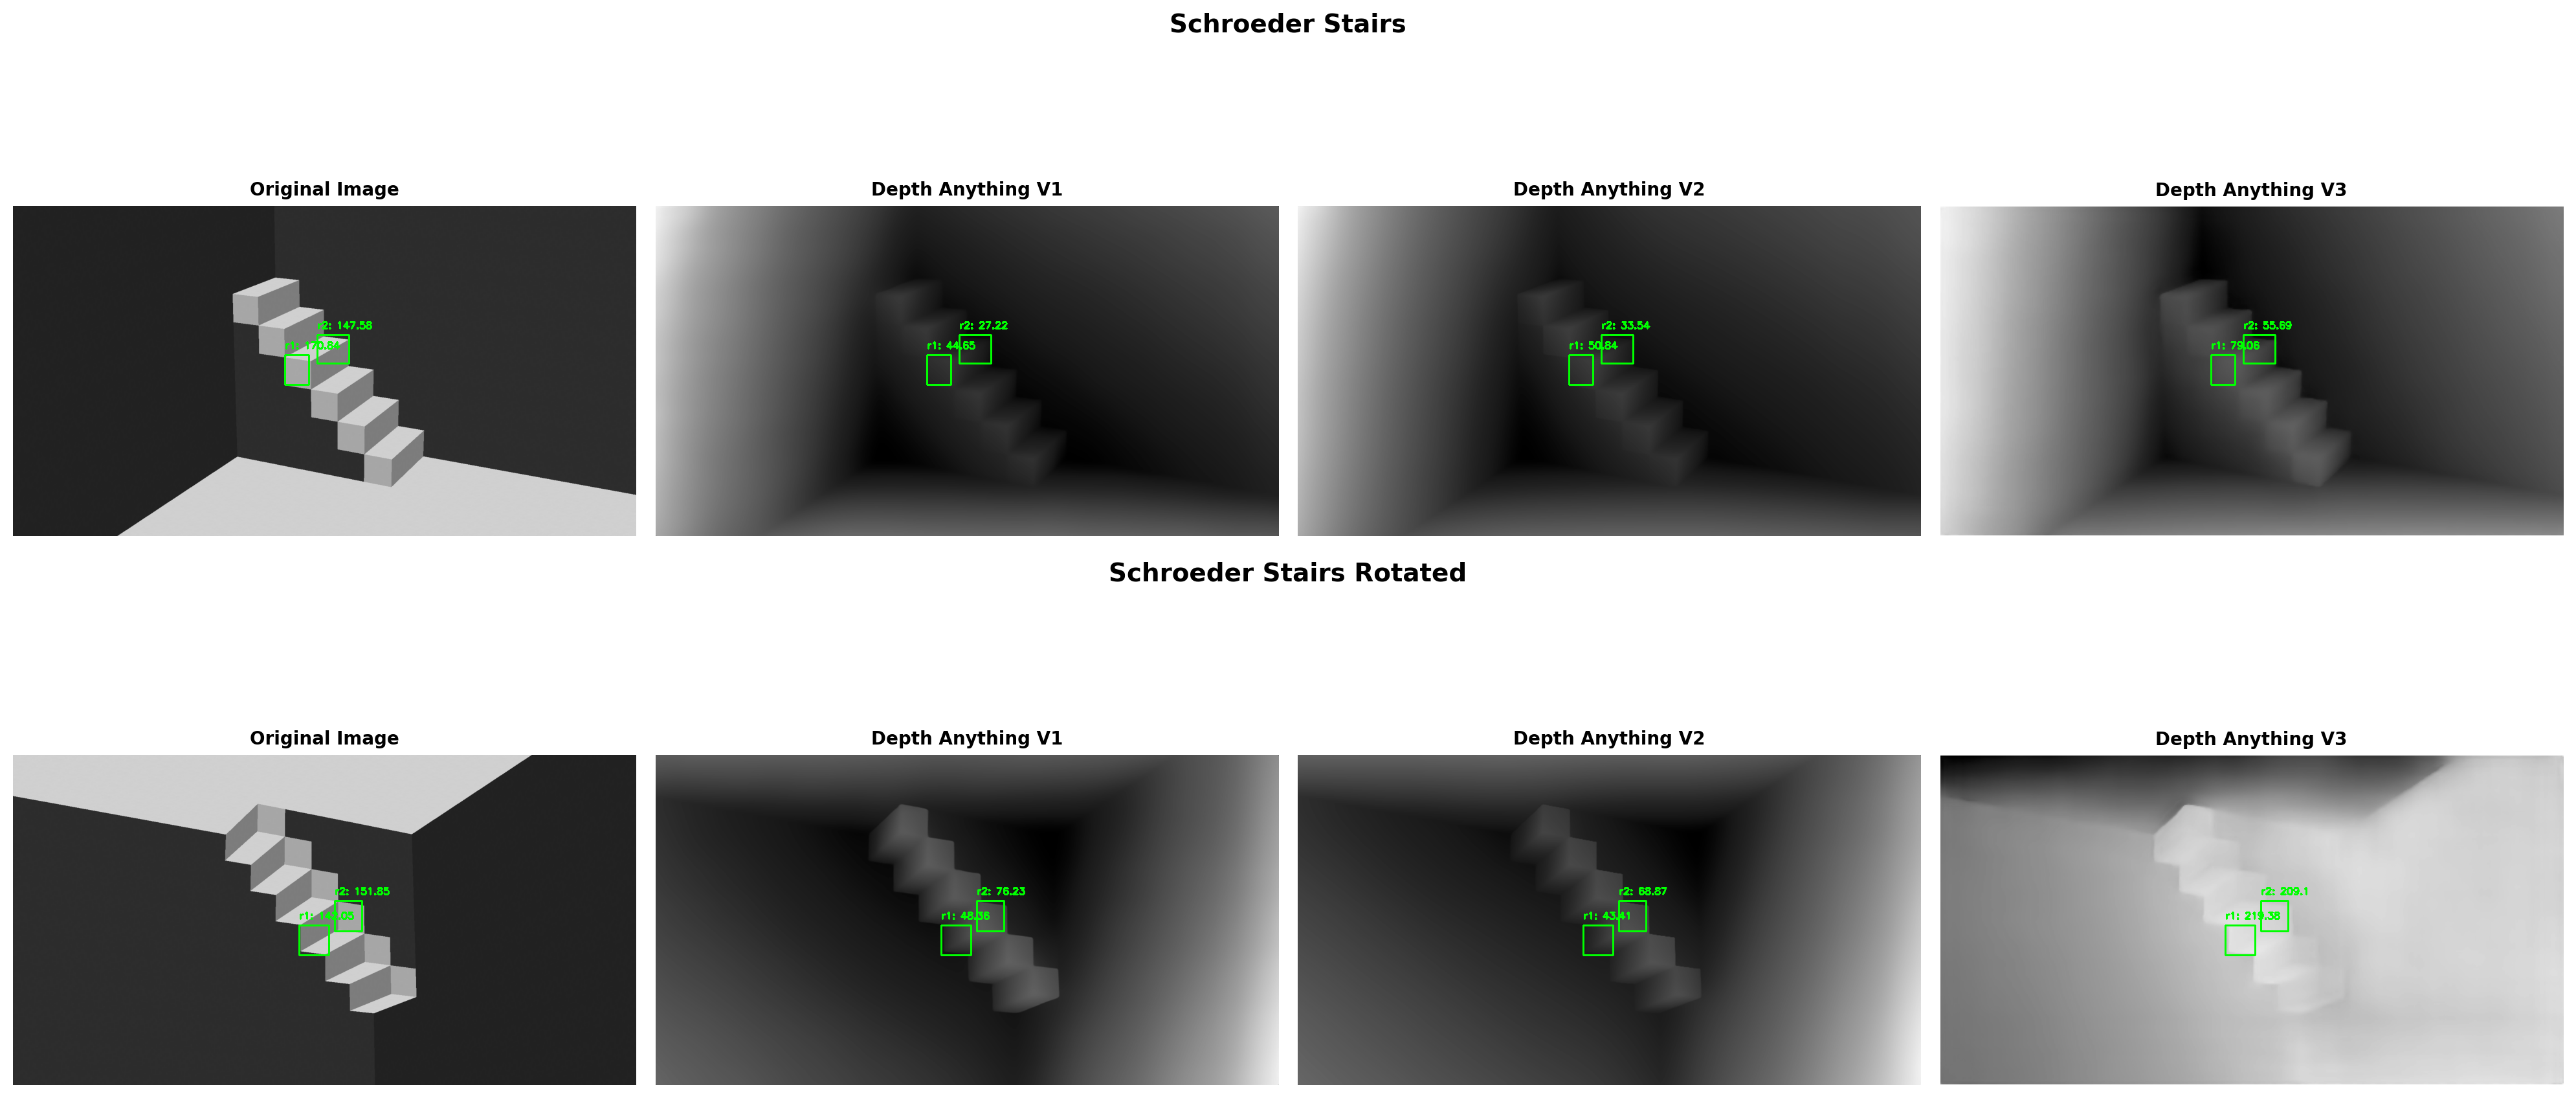
\includegraphics[width=\linewidth]{figures/fig_minecraft_stairs}
  \caption{Schröeder's Stairs rebuilt in the voxel domain, shown upright (top) and
           rotated 180\textdegree{} (bottom). Rotation flips the sign of $\Delta I$ for
           V1 and V2 ($+17 \rightarrow -25$), reversing which step is read as nearer,
           while V3 stays positive ($+10$) in both orientations. This observation suggests that V1/V2 and V3 rely on different structural
           anchors for the same bistable (two interpretations) stimulus.}
  \label{fig:minecraftstairs}
\end{figure}
\subsection{Artificial Psychophysics}

The fifteen psychophysics experiments are grouped, as in the methodology, into
monocular geometric cues, photometric and atmospheric cues, and structural and
semantic cues. Table~\ref{tab:psychophysics} summarizes the PSE and JND extracted for
each model where a clear crossing point could be computed; an entry of n/a indicates
that $\Delta I$ never crossed zero (or never reached the 84\% threshold) within the
30-frame range, which is itself an informative result, since it signals a prior strong
enough that the model never reaches subjective equality for that manipulation.

\textbf{Height Bias (Fig.~\ref{fig:height_bias_sequence}).} A square slides from top to bottom across
30 frames. V1's $\Delta I$ stays positive throughout the entire range and never reaches a
PSE, confirming a height-in-field prior so strong that the model never treats the two
ROIs as equidistant regardless of position. V2 does reach a PSE, but only near the very
end of the range (frame 180 on the extended scale used for this experiment), and its
response is concentrated near the centre of the image, consistent with a centrality
prior rather than a purely vertical one. V3's response is non-linear, reaching a PSE
around frame 93 but with the highest JND recorded in this work (229.1), indicating an
extremely shallow and unstable transition rather than a clean perceptual boundary.

\begin{figure}[htbp]
  \centering
  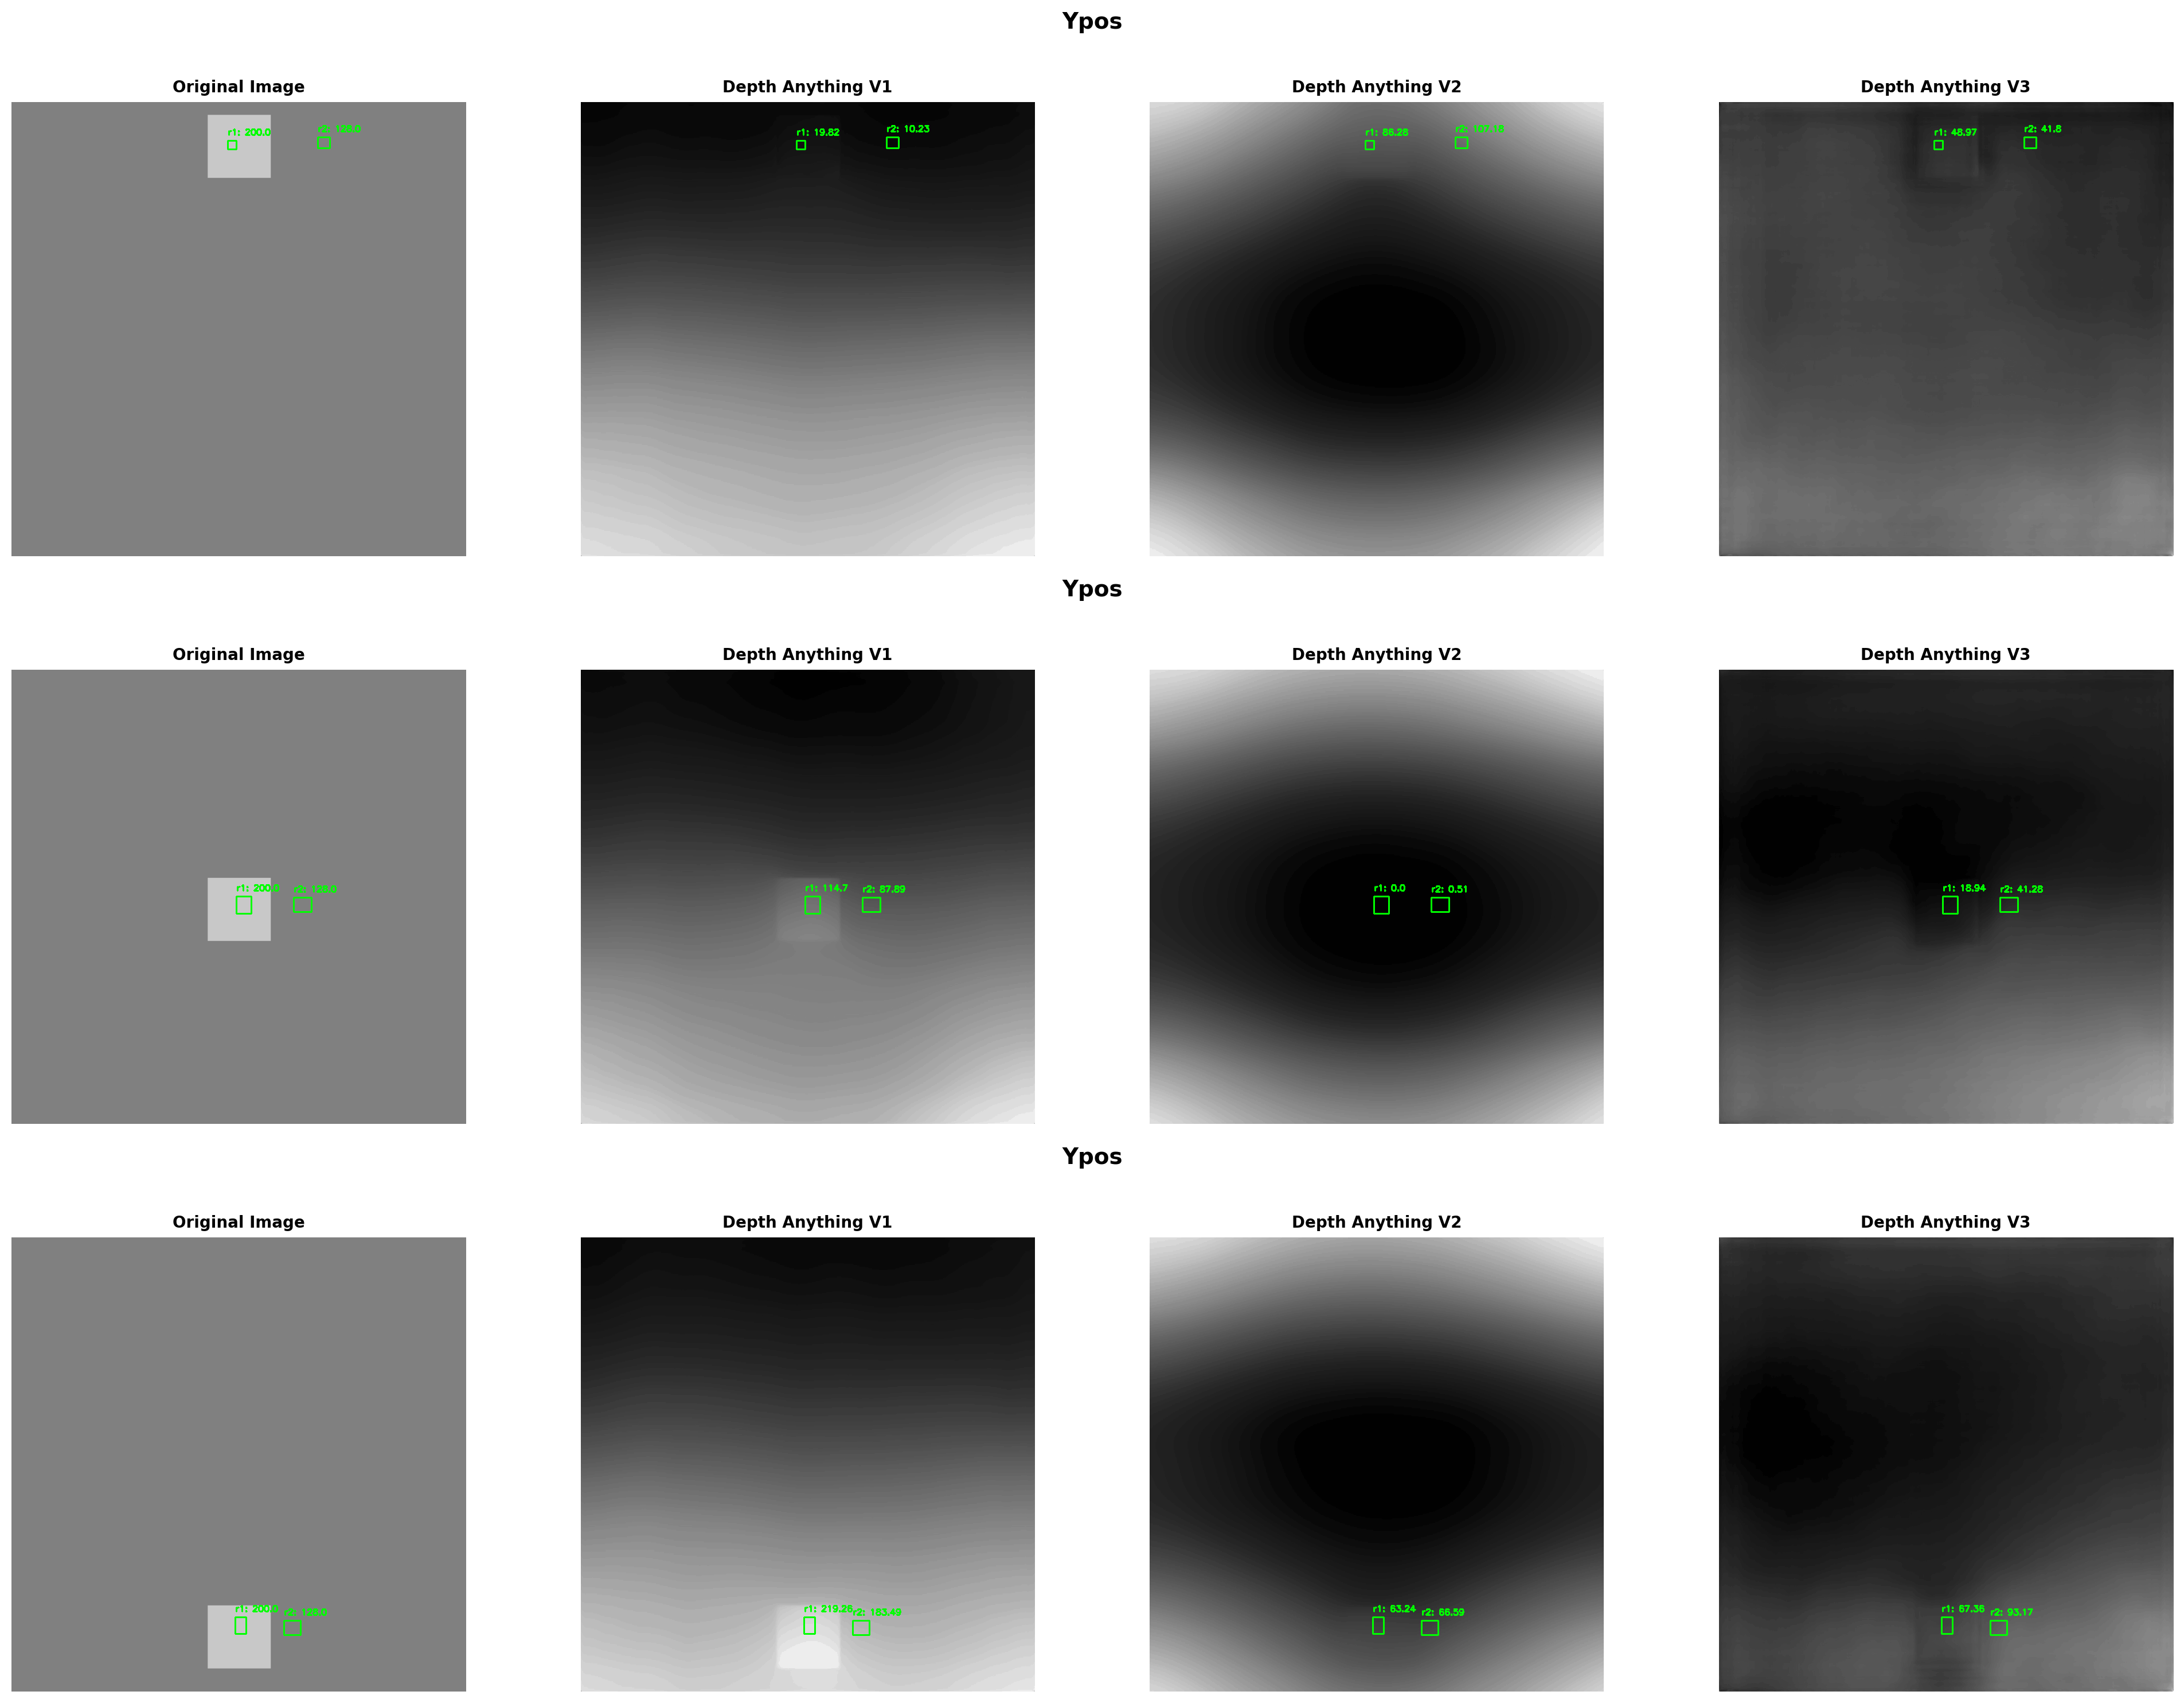
\includegraphics[width=\linewidth]{figures/fig_height_bias}
  \caption{Artificial psychophysics framework illustrated via three representative frames (top, middle, and bottom rows) of the height bias sequence.}
  \label{fig:height_bias_sequence}
\end{figure}

\textbf{Ponzo Bias. (Fig.~\ref{fig:ponzobias})} This is the most consistent experiment across all three models: PSE
occurs within a narrow band around frame 16 to 17 for V1, V2 and V3 alike. What differs
is the steepness of the transition: V1 has the lowest JND (1.27), V2 is close behind
(2.00), and V3, despite reaching the same PSE, has a JND roughly five times larger
(6.66). This suggests that while all three models agree on where the illusion flips, V3's
decision is comparatively less sharp once the local context becomes ambiguous.

\textbf{Horizon Bias.} V1 shows a clean, low-JND ($\text{PSE} = 20.8$, $\text{JND} = 3.0$), indicating a smooth adaptation to the spatial gradient. In contrast, V2 never crosses the zero-boundary within the tested range, as positive values are maintained throughout (0.7 to 56.3); this suggests a rigid, horizon-driven spatial prior that is never addressed by the model. Finally, V3 reaches a similar PSE to V1 ($\text{PSE} = 18.9$), with a significant variability observed ($-196.1$ to $83.4$) (See Fig. \ref{fig:horizon_bias}). 

\textbf{Relative Size.} In the relative-size experiment, V1 and V2 both
reach a PSE (42.2 and 18.5 respectively), with V2's JND roughly 1.7 times larger than
V1's (38.4 vs.\ 23.2), suggesting V2 needs a bigger change in relative size before
committing to a new depth ordering. V3 never crosses zero, staying negative throughout
($-60.4$ to $-0.6$), meaning that within this stimulus range V3 never lets the smaller
object be treated as the closer one (See Fig. \ref{fig:relative_size_bias}). 

\textbf{Texture Gradient.} V1's $\Delta I$ stays negative throughout the full range
($-138.0$ to $-114.1$) and never reaches a PSE, a tight and consistently one-sided
response. V2 and V3 both reach a PSE close to each other (18.7 and 2.7) with comparable
JNDs (9.8 and 11.2), suggesting the two later models treat texture density as a depth
cue in a broadly similar way, in contrast to V1's rigid response (See Fig. \ref{fig:texture_gradient_bias}).

\textbf{Blur Bias.} V1 stays strictly positive across the whole range (13.4 to 130.3) and
V2 stays strictly negative ($-16.3$ to $-5.5$), neither reaching subjective equality. V3
is the only model with a measurable PSE (1.17) and a moderate JND (16.6), reaching
equality almost immediately and then transitioning over a comparatively narrow window.
This is one of the clearest cases in this work of V3 behaving qualitatively differently
from both of its predecessors rather than simply being a refined version of either (See Fig. \ref{fig:blur_bias}).

\textbf{Aerial Perspective.} V1 reaches a PSE around frame 42 with the largest JND
recorded for this model (142.9), indicating a very shallow, almost imperceptible
transition. V2 stays negative throughout and close to zero ($-3.0$ to $-0.1$), suggesting
this contrast-decay cue barely registers for V2 at all. V3 reaches a PSE much later
(126.3) with no measurable JND, again pointing to a noisier and less standard response
than the other geometric-cue experiments (See Fig. \ref{fig:aerial_perspective_bias}).

\textbf{Shading Bias.} V1 stays positive and high throughout (101.9 to 232.9), never
reaching equality, the strongest and most one-sided response among the photometric
cues. V2 reaches a PSE (63.7) but with an extremely large JND (136.0), and a wide range
that crosses from negative to strongly positive ($-55.5$ to $237.9$), suggesting a highly
unstable transition rather than a clean perceptual boundary. V3 stays positive throughout
(127.8 to 185.1), similarly to V1, never reaching subjective equality within this range (See Fig. \ref{fig:shading_bias}).

\textbf{Shadow Attachment Bias.} All three models reach a PSE early in the sequence (V1:
13.0, V2: 5.2, V3: 3.7), but none has a measurable JND, since the transition in each case
happens too abruptly relative to the 84\% threshold criterion to be captured by linear
interpolation between adjacent frames. The clear trend is that each newer model commits
to a depth ordering earlier in the sequence than its predecessor, in line with growing
sensitivity to the shadow as a grounding cue (See Fig. \ref{fig:shadow_attachment_bias}).

\textbf{Kanizsa Bias.} None of the three models reaches subjective equality for the
illusory-contour stimulus. V1 stays positive (38.3 to 146.9), V2 stays negative and large
in magnitude ($-142.3$ to $-57.6$), and V3 stays positive but in a narrower band (44.9
to 92.6) than V1. The fact that V1 and V3 share the same sign while V2 does not suggests
that V2's interpretation of the illusory figure is qualitatively inverted relative to its
neighbours, rather than simply weaker or stronger (See Fig. \ref{fig:kanizsa_bias}).

\textbf{Ebbinghaus Bias.} As with Kanizsa, none of the three models reaches a PSE. V1 and
V3 both stay positive throughout (54.9 to 166.5, and 64.3 to 223.8 respectively), with V3
reaching the highest values recorded in this experiment; V2 stays negative throughout
($-168.5$ to $-66.1$). The size-contrast manipulation behind the Ebbinghaus illusion
therefore produces a strong and stable bias in all three models, but with V2 disagreeing
in sign with V1 and V3, mirroring the pattern seen for Kanizsa (See Fig. \ref{fig:ebbinghaus_bias}).

\textbf{Hollow Face Bias.} Curves are far from the equality point for V1 and V2, which
never reach a PSE (ranges 13.3 to 197.5, and 37.5 to 164.5 respectively). V3 does reach a
PSE (15.6), and its maximum confusion occurs when the face is completely flat, the point
at which the convexity cue that normally drives the hollow-face illusion disappears
entirely (See Fig. \ref{fig:hollow_face_bias}).

\textbf{Figure-Ground Bias.} This is the experiment with the lowest JND recorded for V1
in this work (2.72, PSE $=4.86$), indicating an extremely sharp transition between the
two interpretations of the ambiguous figure. V2 reaches a similar PSE (11.4) without a
measurable JND, and V3 reaches an even earlier PSE (1.06) with a comparatively higher
JND (24.7), again suggesting that V3's decision, although fast to start, resolves more
gradually than V1's (See Fig. \ref{fig:figure_ground_bias}). \newline

\textbf{Occlusion Bias.} V1 never reaches a PSE, staying negative throughout ($-85.9$ to
$-55.7$). V2 reaches a PSE late in the sequence (19.8) without a measurable JND, while V3
reaches a much earlier PSE (5.4, JND $=23.0$), indicating that between roughly frame 4
and frame 6 the model flips its depth assignment as the overlapping square's transparency
crosses the midpoint (See Fig. \ref{fig:occlusion_bias}).

\begin{table}[htbp]
\centering
\caption{Point of Subjective Equality (PSE) and Just Noticeable Difference (JND) for
Depth Anything V1, V2 and V3 across the fifteen psychophysics experiments. An entry of
n/a means $\Delta I$ either never crossed zero or never reached the 84\% threshold within
the 30-frame range tested.}
\label{tab:psychophysics}

\resizebox{\columnwidth}{!}{%
\begin{tabular}{lccc}
\toprule
\textbf{Experiment} & \textbf{V1 (PSE/JND)} & \textbf{V2 (PSE/JND)} & \textbf{V3 (PSE/JND)} \\
\midrule
Height        & n/a / n/a     & 180.2 / n/a   & 93.1 / 229.1 \\
Ponzo         & 16.6 / 1.3    & 16.6 / 2.0    & 16.5 / 6.7 \\
Horizon       & 20.8 / 3.0    & n/a / n/a     & 18.9 / n/a \\
Relative size & 42.2 / 23.2   & 18.5 / 38.4   & n/a / n/a \\
PSE conflict  & 9.6 / n/a     & 0.8 / 16.9    & 17.8 / n/a \\
Texture grad. & n/a / n/a     & 18.7 / 9.8    & 2.7 / 11.2 \\
Blur          & n/a / n/a     & n/a / n/a     & 1.2 / 16.6 \\
Aerial persp. & 42.4 / 142.9  & n/a / n/a     & 126.3 / n/a \\
Shading       & n/a / n/a     & 63.7 / 136.0  & n/a / n/a \\
Shadow attach.& 13.0 / n/a    & 5.2 / n/a     & 3.7 / n/a \\
Kanizsa       & n/a / n/a     & n/a / n/a     & n/a / n/a \\
Ebbinghaus    & n/a / n/a     & n/a / n/a     & n/a / n/a \\
Hollow face   & n/a / n/a     & n/a / n/a     & 15.6 / n/a \\
Figure-ground & 4.9 / 2.7     & 11.4 / n/a    & 1.1 / 24.7 \\
Occlusion     & n/a / n/a     & 19.8 / n/a    & 5.4 / 23.0 \\
\bottomrule
\end{tabular}%
}
\end{table}

\begin{figure}[H]
  \centering
  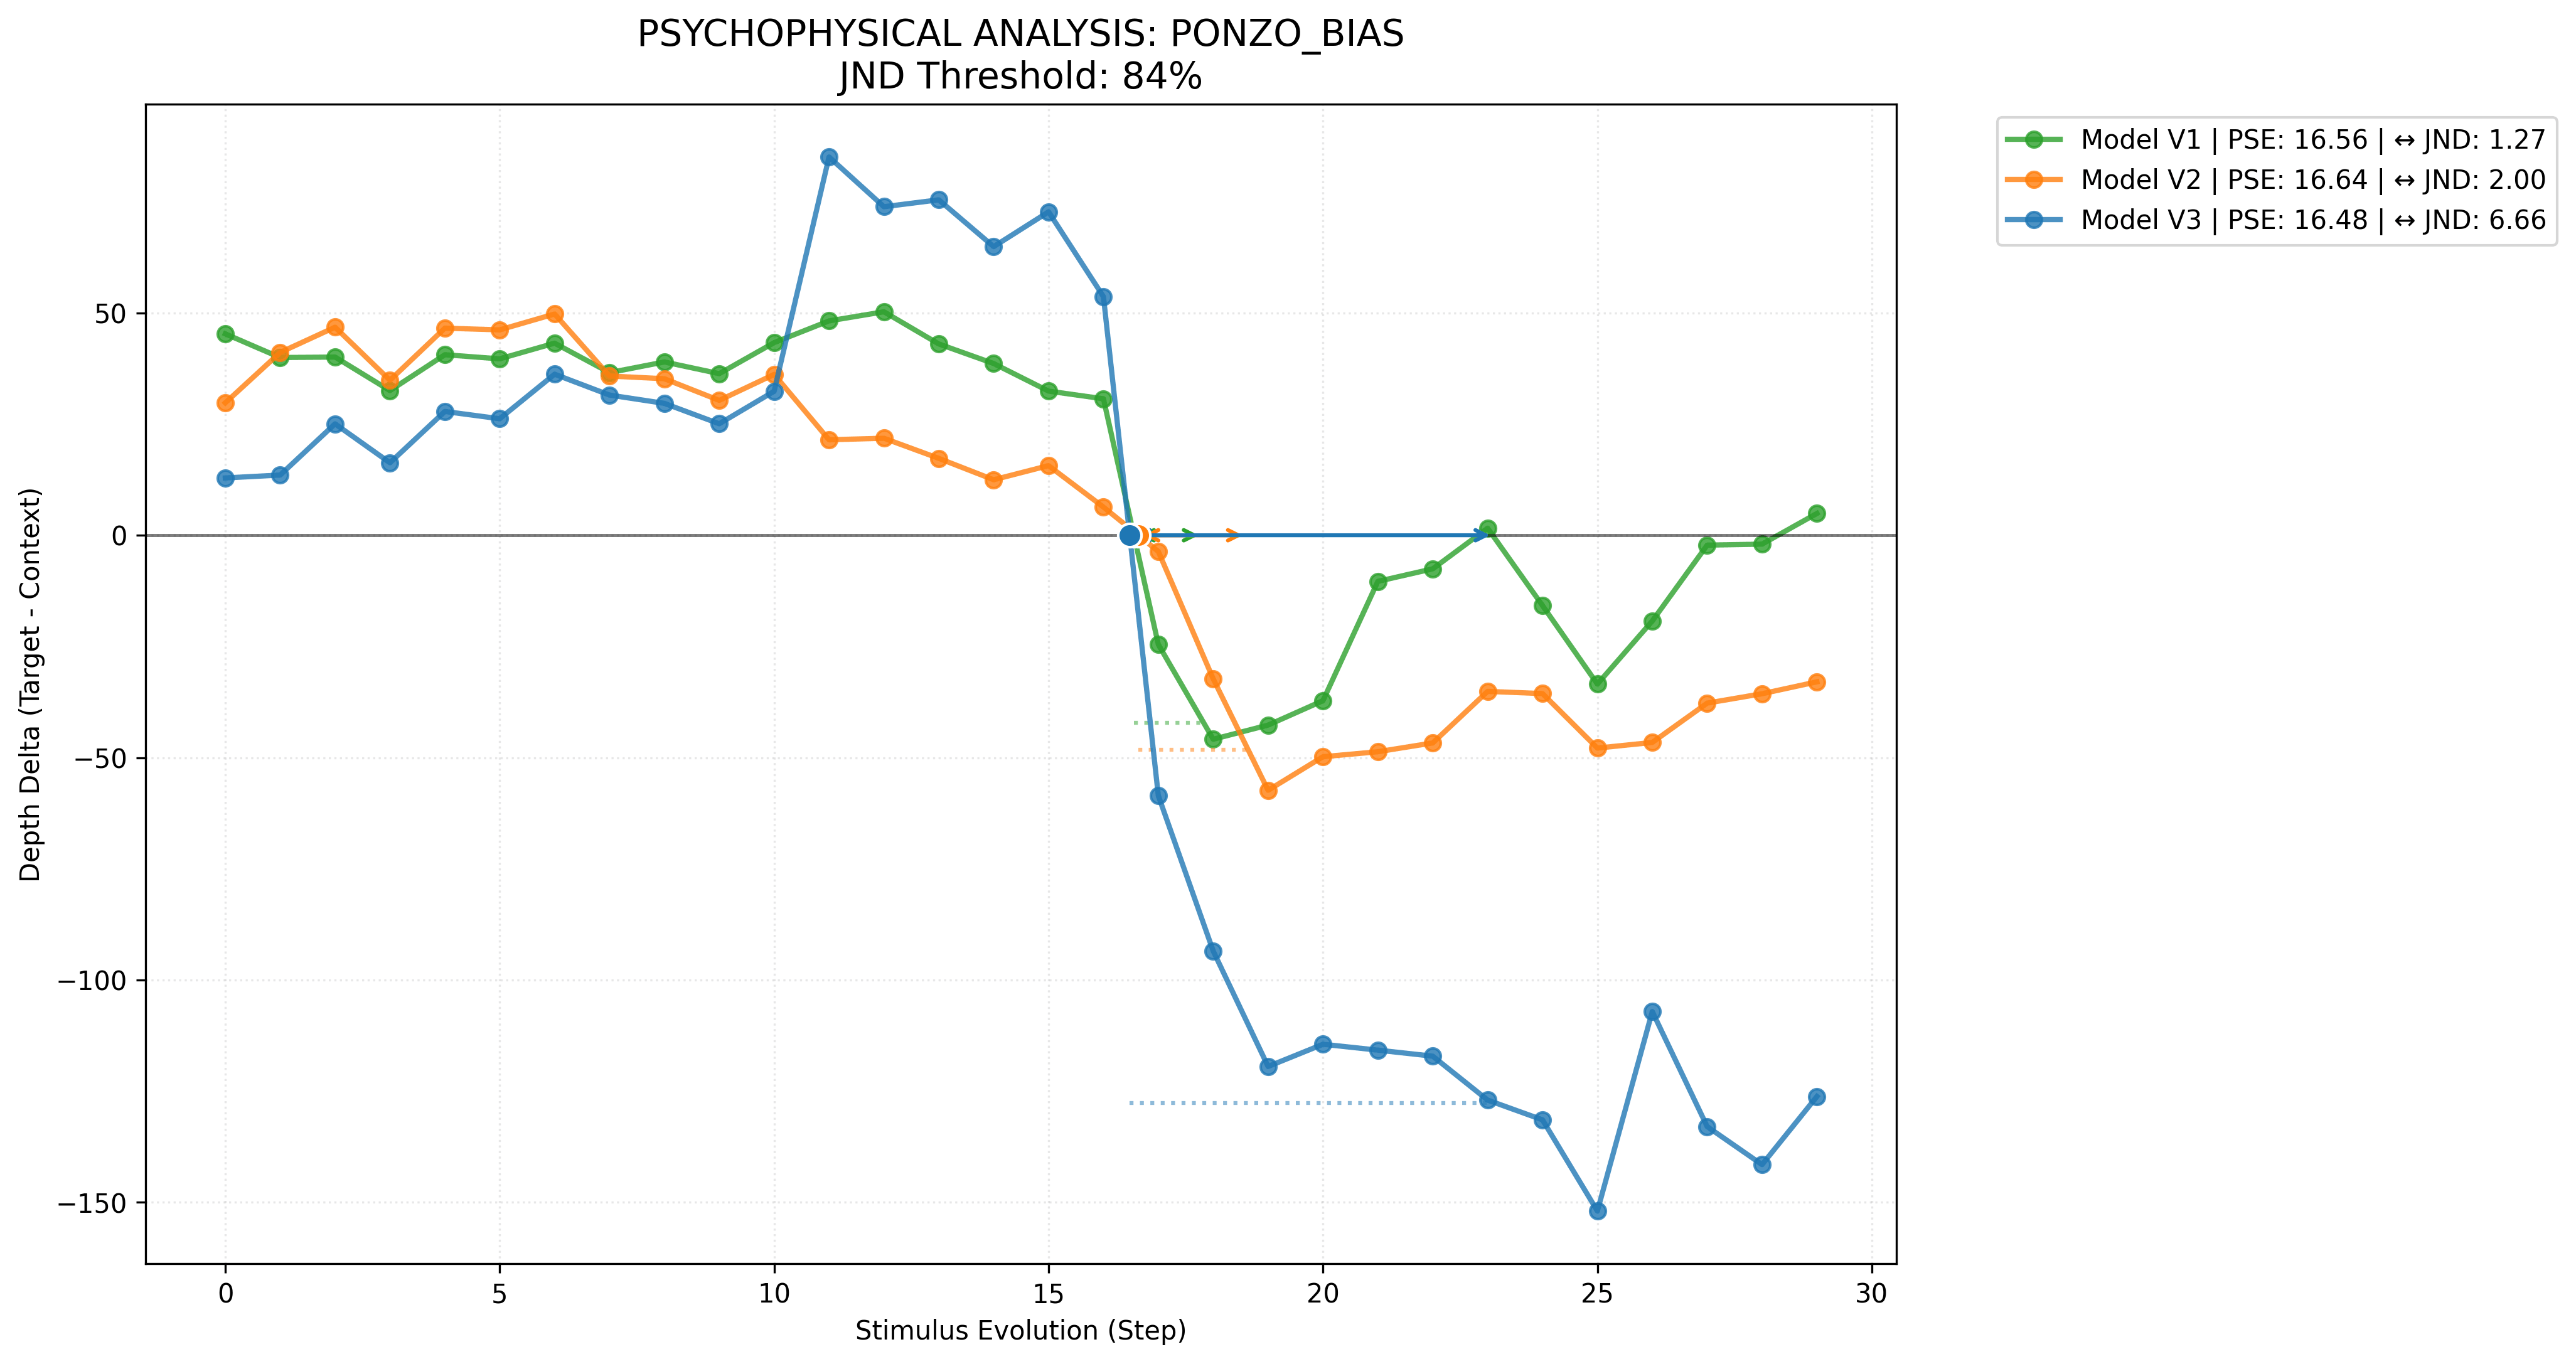
\includegraphics[width=\linewidth]{figures/fig_ponzo_bias}
  \caption{Ponzo bias experiment. All three models exhibit a highly consistent Point of Subjective Equality (PSE) around frames 16--17. However, transition steepness varies significantly: V1 and V2 display sharp transitions (low JND), whereas V3 exhibits a much larger JND, indicating a less sharp decision boundary once local context becomes ambiguous.}
  \label{fig:ponzobias}
\end{figure}

\subsection{Cross-Architecture Comparison: MiDaS}
\label{sec:midas}

To assess whether the identified biases are specific to the Depth Anything ViT
architecture or are more general to monocular depth estimation, the CNN-based
MiDaS model~\cite{ranftl2020} is evaluated on the same baseline dataset, the same
Corridor Illusion ablation, the same voxel laboratory, and the same psychophysics
protocol used for V1, V2 and V3.

\textbf{Qualitative behaviour on classical illusions.} On the Necker Cube, MiDaS
does not attempt to resolve the ambiguity at all. Rather than committing to either
orientation, it produces a smooth depth gradient running from dark at the top to
bright at the bottom, effectively ignoring the cube's geometry and applying its
default positional prior on top of it (See Fig.~\ref{fig:necker_cube_midas}). The same gradient dominates the Ponzo and
Corridor illusions: the upper bar and the upper cylinder are pushed to a darker
(farther) value purely because of where they sit in the frame, independently of the
converging lines around them. On Escher's Cube, MiDaS does not merge the
intersection the way V1 and V2 do, nor does it generate the high-contrast artifacts
seen in V3. It simply lights up every edge of the cube with similar intensity,
suggesting that, when faced with an impossible structure, the model falls back to
treating the image as a flat, high-contrast pattern rather than attempting any 3D
interpretation. The hollow-face prior is replicated as expected: both the convex
and the concave mask in the Hollow Face stimulus are predicted as bulging towards
the camera. Fig.~\ref{fig:midascorridor} shows MiDaS's output on the Corridor
Illusion and Escher's Cube.

\begin{figure}[H]
  \centering
  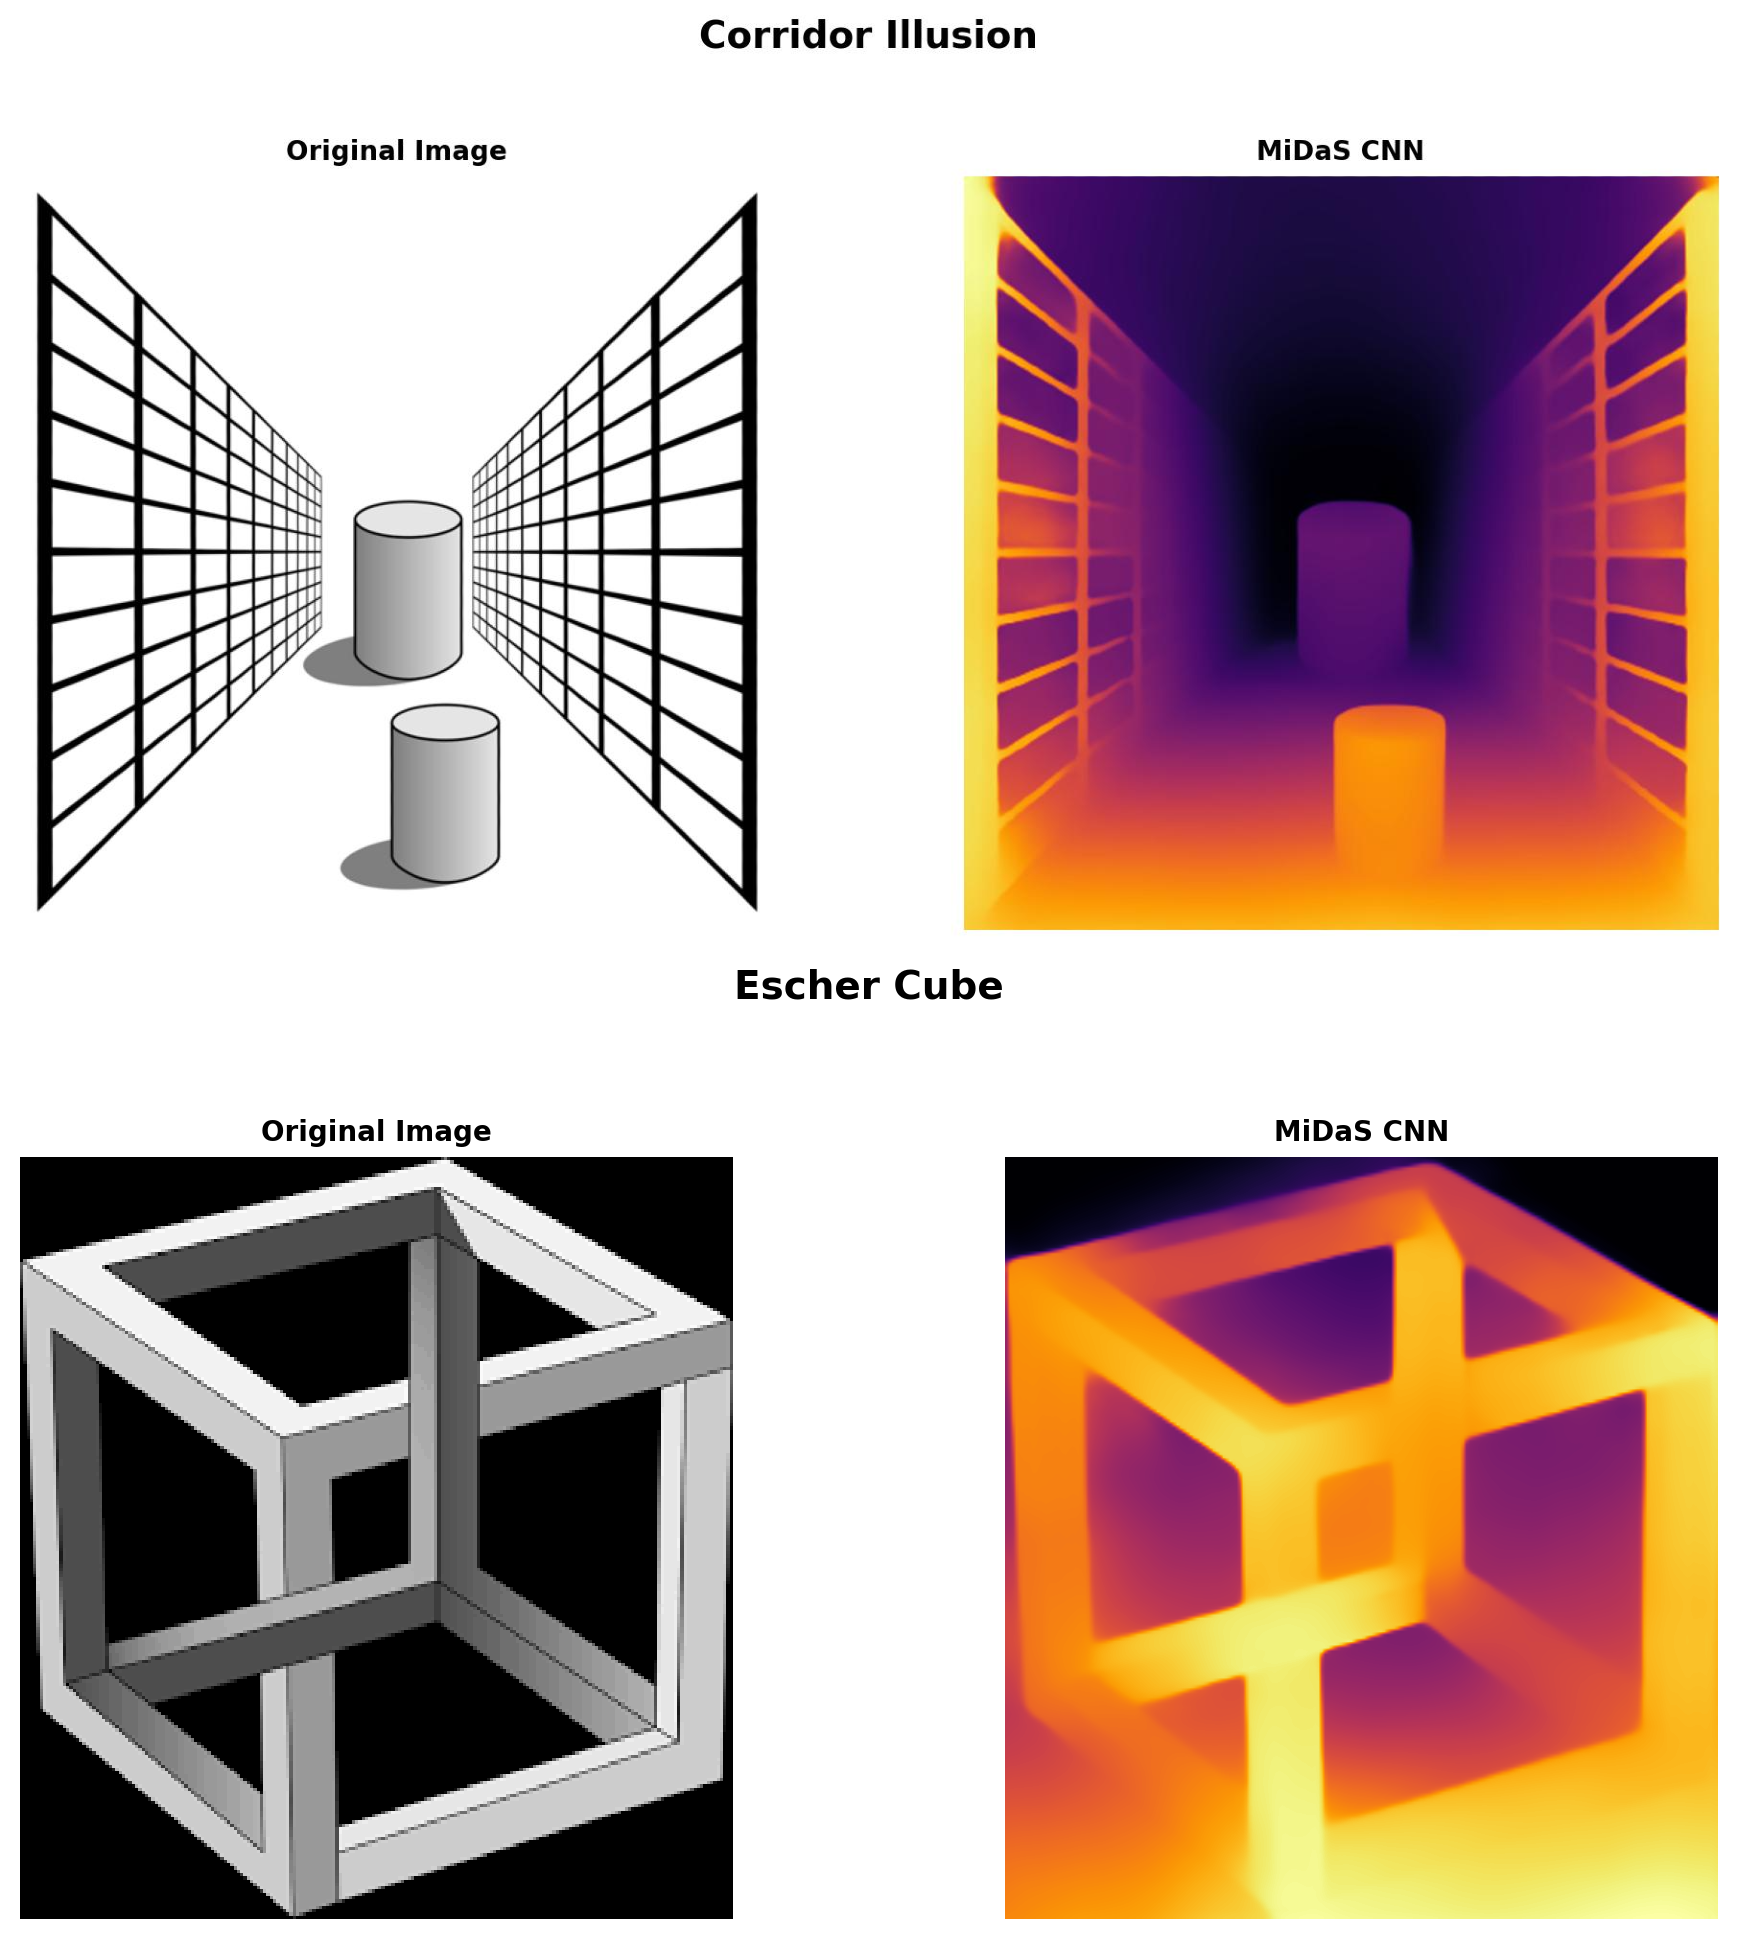
\includegraphics[width=\linewidth]{figures/fig_midas_corridor}
  \caption{Corridor Illusion and Escher's Cube processed by MiDaS. The height-driven
           gradient on the Corridor mirrors V1's behaviour; on Escher's Cube, MiDaS lights
           up every edge with similar intensity rather than fusing faces (as V1 and V2 do)
           or fracturing the structure (as V3 does).}
  \label{fig:midascorridor}
\end{figure}

\textbf{Synthetic Stimuli Engineering.} Table~\ref{tab:corridor} includes MiDaS
alongside V1, V2 and V3 for all fifteen Corridor Illusion variants. The pattern
that emerges is consistent with the qualitative observations above: MiDaS is the
model least affected by the removal of contextual cues. ``Only Cylinders,'' which
strips away the walls, the floor and the grid, reduces V2 to $\Delta I = 11.9$ and
V3 to $6.4$, but barely moves MiDaS, which stays at $71.4$, one of its higher
values in the whole table. The same pattern holds for the high-low frequency
split, where mixing low- and high-frequency content on the two cylinders collapses
V3 to $13.6$ while MiDaS remains at $77.2$. MiDaS is also insensitive to object
orientation in a way the other three models are not: the Shepard Illusion, which
rotates the cylinder horizontally and weakens the bias substantially for V1, V2 and
V3 (down to 17 to 27), produces the highest $\Delta I$ recorded for MiDaS in the
entire ablation ($139.6$). The mean $\Delta I$ across all fifteen variants is
$85.0$ for MiDaS, with a minimum of $30.9$ (Minecraft transfer) and a maximum of
$152.1$ (Cube Walls). Taken together, this points to a height-in-field prior that
is considerably more rigid than V1's: where V1's bias weakens once enough context
is removed, MiDaS's bias stays roughly constant regardless of what is removed.

\textbf{Voxel laboratory.} The same resistance to context removal is visible in
the Minecraft experiments. Forced perspective stimuli (fake block, depth
incongruence, anamorphic cube) (\cref{fig:fig_fake_block,fig:fig_depth_incongruence,fig:fig_anamorphic_cube}) give MiDaS the lowest average $\Delta I$ of any
category ($7.9$), confirming that resistance to forced-perspective tricks is not
unique to ViT-based architectures. Depth ambiguity stimuli average $34.1$, with
the Necker Cube again standing out at $75.4$, the same non-resolution behaviour
seen in the photographic dataset. Impossible objects average $41.0$, with Penrose
Triangle (zoomed) and Escher's Waterfall producing the largest gaps ($94.7$ and
$78.3$); rather than producing artifacts when the geometry cannot be resolved, as
V3 does, MiDaS appears to simply apply its dominant positional prior without any
visible attempt at reconciling the impossibility. Shading stimuli show the widest
spread of any category, from $1.9$ (dragon) to $127.6$ (concave-convex furnace,
zoomed), suggesting that MiDaS's shape-from-shading response depends heavily on
scene-specific factors such as scale rather than on a single stable prior.
Converging-lines stimuli show a similarly wide spread (1.5 to 160.4), the largest
range of any model evaluated in this domain.

\begin{table}[h]
\centering
\caption{Point of Subjective Equality (PSE) and Just Noticeable Difference (JND) for
MiDaS, computed with the same protocol as Table~\ref{tab:psychophysics} across the same
fifteen experiments. An entry of n/a in the PSE column means $\Delta I$ never crossed
zero within the tested range; the range column reports where it stayed instead. An
entry of n/a in the JND column means the curve never reached the 84\% threshold needed
to compute it, even though a PSE was found.}
\label{tab:psychophysics_midas}
\small
\begin{tabular}{lccc}
\toprule
\textbf{Experiment} & \textbf{PSE} & \textbf{JND} & \textbf{Range} \\
\midrule
Angle              & 55.5 & 108.3 & --- \\
Blur bias          & 16.1 & 11.5  & --- \\
Aerial Perspective          & 205.4 & n/a  & --- \\
Ebbinghaus         & n/a  & n/a   & 88--233 \\
Shading       & 19.6 & n/a   & --- \\
Figure-ground      & 18.0 & 5.2   & --- \\
Horizon            & 0.9  & 21.8  & --- \\
Kanizsa            & n/a  & n/a   & 22--97 \\
Occlusion          & 22.8 & 5.8   & --- \\
Ponzo              & 17.3 & 2.3   & --- \\
Shadow attachment         & 5.1  & n/a   & --- \\
Relative Size               & n/a  & n/a   & 16--122 \\
PSE conflict & n/a  & n/a   & 18--106 \\
Texture gradient      & n/a  & n/a   & 93--195 \\
Height               & n/a  & n/a   & 27--182 \\
\bottomrule
\end{tabular}
\end{table}

\textbf{Psychophysics.} Table~\ref{tab:psychophysics_midas} reports PSE and JND for
MiDaS across all fifteen experiments. Five categories never cross zero within the
30-frame range tested: ypos, size, size\_vs\_position, texture\_slant, and kanizsa.
For the first three, $\Delta I$ stays strictly positive throughout (ranges of 26.8 to
181.6, 15.8 to 122.3, and 17.8 to 105.6 respectively), a stronger and more rigid prior
than what V1 shows on the equivalent experiment, where the curve eventually reaches a
crossing point. Ebbinghaus shows the same one-sided behaviour (88.4 to 233.1), pointing
to a stable size-contrast bias that is never neutralised within this range.

A second group reaches a PSE but without a measurable JND, since the transition is too
abrupt relative to the 84\% threshold criterion: contrast (PSE $=205.4$), face shading
(PSE $=19.6$), and shadow gap (PSE $=5.1$). The early PSE for shadow gap in particular
suggests that MiDaS commits to a depth ordering based on the shadow cue almost
immediately once it appears, similarly to the early commitment seen for V3 on the
equivalent shadow-attachment experiment.

The remaining six categories produce a measurable PSE together with a JND. Ponzo shows
the most extreme transition of the whole set (JND $= 2.32$), where $\Delta I$ flips from
around $+25$ to $-200$ within a handful of frames rather than transitioning gradually.
Occlusion (PSE $=22.8$, JND $=5.8$) and figure-ground (PSE $=18.0$, JND $=5.2$) are
comparatively sharp as well, while blur bias (PSE $=16.1$, JND $=11.5$) and horizon
(PSE $=0.9$, JND $=21.8$) show progressively shallower transitions. Angle is the
noisiest of the group (PSE $=55.5$, JND $=108.3$), with $\Delta I$ oscillating
repeatedly between positive and negative values rather than following a single clear
trend, which inflates the JND well beyond anything observed for V1, V2 or V3 on a
comparable experiment.

Overall, MiDaS's psychophysical responses are considerably more variable in shape from
one experiment to another than those of V1, V2 or V3: some categories (Ponzo, occlusion,
figure-ground) show sharp, almost categorical transitions, while others (angle, several
of the position- and size-related stimuli) never resolve into a clean crossing at all.
Despite this variability, the underlying positional bias, when it is present, tends to be
at least as strong as V1's, and in several cases (ypos, size\_vs\_position) considerably
more rigid.

In summary, MiDaS exhibits a height-in-field prior that is qualitatively similar
to V1's but quantitatively more rigid: it is largely indifferent to the contextual
manipulations (walls, frequency content, object orientation, semantic identity)
that substantially weaken or even collapse the bias in V2 and especially V3. This
is consistent with the idea that the convolutional backbone encodes a more local,
position-dependent notion of depth, while the richer context integration observed
in V3 appears to be tied to the larger-scale, semi-supervised ViT training regime
rather than to monocular depth estimation in general.

% ============================================================
\section{Discussion}
\label{sec:discussion}

\textbf{V1} is governed by a primitive \textbf{height-in-field prior}: vertical position is
the dominant depth cue, replicating a fundamental human prior (objects higher in the
visual field tend to be farther away). This prior persists even under heavy context removal.

\textbf{V2} transitions to a \textbf{centrality prior}: objects closer to the image centre
are predicted as farther. This shift is consistent with training on photographic datasets
where subjects of interest tend to be centred, creating an implicit statistical regularity.

\textbf{V3} exhibits \textbf{context-driven global geometry}: it integrates converging
lines, shading, textures, and object borders more aggressively than predecessors. This
produces the highest susceptibility under full-cue conditions, but collapses to near-zero
$\Delta I$ when cues are stripped, a hallmark of a model that has learned richer but
more brittle representations.

The cross-domain voxel experiments further support that these priors are structural rather than texture-dependent. Depth biases persist in discrete environments with comparable sign and magnitude, reinforcing the hypothesis that these effects arise from architectural inductive biases rather than surface-level visual statistics.

Critically, the cross-architecture comparison shows that the evaluated CNN-based model MiDaS shares V1's
height-in-field prior but in a more rigid form: across the Corridor Illusion
ablation, MiDaS keeps a similar $\Delta I$ regardless of which cue is removed,
while V1's bias does weaken somewhat once enough context disappears.  This may indicate that the positional, height-driven notion of depth observed in MiDaS may be linked to its specific convolutional architecture, while the centrality prior of V2 and
the strong but fragile  context integration of V3 look more like properties that
emerge specifically from large-scale ViT training rather than from monocular
depth estimation as a task.

% ============================================================
\section{Conclusions}
\label{sec:conclusions}

This work demonstrates that modern monocular depth estimation models are
systematically vulnerable to 3D optical illusions, revealing consistent and
measurable biases across architectures. The results indicate that different
model families develop distinct priors that influence depth perception, with
notable differences between convolutional and transformer-based systems.
Furthermore, architectural design plays a key role in shaping the trade-off
between semantic understanding and geometric robustness. Finally, the study
highlights that these biases are structural rather than data-dependent, as they
persist across synthetic voxel environments. Table~\ref{tab:model_priors_summary} condenses these findings into a single comparison across all four models. \newline


\begin{table}[htbp]
\centering
\caption{Summary of primary priors, robustness under isolated conditions, and susceptibility to full contextual illusions across MDE models.}
\label{tab:model_priors_summary}
\small
\begin{tabular}{p{1cm}p{2.5cm}cc}
\toprule
\textbf{Model} & 
\textbf{Primary prior} & 
\textbf{\parbox[c]{1.6cm}{\centering Robustness\\(no context)}} & 
\textbf{\parbox[c]{1.8cm}{\centering Susceptibility\\(full context)}} \\
\midrule
V1& Height-in-field             & High & Moderate \\
V2& Centrality                  & High & Moderate to high \\
V3& Global context integration  & Low  & High \\
MiDaS& Height-in-field             & High & Moderate \\
\bottomrule
\end{tabular}
\end{table}
\subsection*{Implications}

These findings have direct safety implications. A model with a strong height bias (V1,
MiDaS) will systematically misestimate the depth of objects in atypical vertical positions.
A context-driven model (V3) may be vulnerable to adversarial removal of cues. Both
failure modes are relevant for deployment in robotics and autonomous systems.

\subsection*{Limitations}

There are several limitations that must be acknowledged.

The dataset was curated to maintain structural diversity across the taxonomy
rather than to reflect the real-world frequency of these ambiguities and
should not be read as representative of how often such illusions occur outside
a controlled setting.

The ROI extraction uses the mean intensity of the region, mitigating noise and
local artifacts, but the bounding box itself is placed manually, introducing a
small amount of subjectivity and bias that is not currently quantified.

Only one CNN-based model has been analyzed; generalizing the behavior of
convolutional architectures against 3D visual illusions would require testing
additional CNN-based models.

All fifteen artificial psychophysics stimuli are synthetic, parametrically
generated sequences designed to vary a single cue in isolation, and may
therefore not correlate with how these cues co-occur and interact in natural
images.

Finally, due to hardware constraints, the evaluation of the Depth Anything
family and MiDaS was restricted to their "Base" variants; larger variants
could possess greater representational capacity and may exhibit different
biases.

\subsection*{Future Work}

Several directions remain open: (1) evaluation of diffusion-based depth models such as
Marigold~\cite{marigold2024}, hypothesised to exhibit context-integration properties similar to V3; (2) investigation of adversarial stimuli designed to maximally exploit the
identified priors; and (3) human psychophysics studies to directly compare the PSE/JND
thresholds of models and biological observers.

% ============================================================
\section*{Acknowledgements}

The author thanks Alexandra Gomez Villa for her guidance and feedback throughout
the project. Computational support for high-parameter generative models was provided
by Hugging Face ZeroGPU Spaces~\cite{zerogpu}.

The author would also like to thank his mother and sister, his partner, and his friends
for their patience and support throughout the development of this project.

\section*{Use of Generative AI}

A generative AI assistant was used during the writing of this report to help with
language editing and rephrasing, to search for and explain background concepts
referenced in the State of the Art, and to clarify terminology when needed. All research
design, experiments, code, data analysis, results, and conclusions presented in this work
are the author's own.

% ============================================================
\bibliographystyle{IEEEtran}
% Use \bibliography{references} if you have a .bib file,
% or use the inline bibliography below.

\begin{thebibliography}{99}

\bibitem{gregory1997}
R. L. Gregory, ``Knowledge in perception and illusion,''
\emph{Phil. Trans. R. Soc. Lond. B}, vol.~352, no.~1358,
pp.~1121--1128, 1997.

\bibitem{hubel1962}
D. H. Hubel and T. N. Wiesel, ``Receptive fields, binocular interaction and
functional architecture in the cat's visual cortex,''
\emph{J. Physiol.}, vol.~160, no.~1, pp.~106--154, 1962.

\bibitem{kitaoka2005}
A. Kitaoka, H. Ashida, and I. Murakami, ``Does the peripheral drift illusion
generate illusory motion in depth?'' Ritsumeikan University, 2005.

\bibitem{conway2005}
B. R. Conway, A. Kitaoka, A. Yazdanbakhsh, C. C. Pack, and M. S. Livingstone,
``Neural basis for a powerful static motion illusion,''
\emph{J. Neurosci.}, vol.~25, no.~23, pp.~5651--5656, 2005.

\bibitem{sugihara2015}
K. Sugihara, ``Ambiguous cylinders: a new class of impossible objects,''
\emph{CADDM}, vol.~25, no.~4, pp.~19--25, 2015.

\bibitem{gomezVilla2025}
A. Gomez-Villa et al., ``The art of deception: Color visual illusions and diffusion
models,'' in \emph{Proc. IEEE/CVF CVPR}, 2025.

\bibitem{ngo2023}
J. Ngo, S. Sankaranarayanan, and P. Isola, ``Is CLIP fooled by optical illusions?''
\emph{ICLR Tiny Papers}, 2023.

\bibitem{ranftl2020}
R. Ranftl, K. Lasinger, D. Hafner, K. Schindler, and V. Koltun,
``Towards robust monocular depth estimation: Mixing datasets for zero-shot
cross-dataset transfer,'' \emph{IEEE TPAMI}, vol.~44, no.~3, pp.~1623--1637, 2020.

\bibitem{depthanythingv1}
L. Yang et al., ``Depth anything: Unleashing the power of large-scale unlabeled
data,'' in \emph{Proc. IEEE/CVF CVPR}, 2024.

\bibitem{depthanythingv2}
L. Yang et al., ``Depth anything V2,'' in \emph{NeurIPS}, 2024.

\bibitem{depthanythingv3}
Depth Anything Team, ``Depth Anything V3,''
\url{https://depth-anything-3.github.io}, 2025.

\bibitem{gescheider1997}
G. A. Gescheider, \emph{Psychophysics: The Fundamentals}.
Lawrence Erlbaum Associates, 1997.

\bibitem{wichmann2001}
F. A. Wichmann and N. J. Hill, ``The psychometric function: I. Fitting, sampling,
and goodness of fit,'' \emph{Percept. Psychophys.}, vol.~63, no.~8,
pp.~1293--1313, 2001.

\bibitem{hunyuan3d}
Tencent Hunyuan Team, ``Hunyuan3D 2.0: Scaling diffusion models for high
resolution textured 3D assets generation,'' arXiv:2501.12202, 2025.

\bibitem{zerogpu}
Hugging Face, ``ZeroGPU Spaces,''
\url{https://huggingface.co/docs/hub/en/spaces-zerogpu}, 2026.

\bibitem{minecraft2011}
Mojang Studios, \emph{Minecraft} [Video game], 2011.
\url{https://www.minecraft.net}

\bibitem{fechner1860}
G. T. Fechner, \emph{Elemente der Psychophysik}.
Breitkopf u. Härtel, 1860.

\bibitem{necker1832}
L. A. Necker, ``Observations on some remarkable optical phenomena seen in
Switzerland; and on an optical phenomenon which occurs on viewing a figure
of a crystal or geometrical solid,'' \emph{London and Edinburgh Phil. Mag. and
J. of Science}, vol.~1, no.~5, pp.~329--337, 1832.

\bibitem{ponzo1911}
M. Ponzo, ``Intorno ad alcune illusioni nel campo delle sensazioni tattili,
sull'illusione di Aristotele e fenomeni analoghi,''
\emph{Rendiconti della Accademia delle Scienze di Torino}, vol.~58, 1911.

\bibitem{ittelson1952}
W. H. Ittelson, \emph{The Ames Demonstrations in Perception: A Guide to their
Construction and Use}. Princeton University Press, 1952.

\bibitem{ramachandran1988}
V. S. Ramachandran, ``Perception of shape from shading,''
\emph{Nature}, vol.~331, no.~6152, pp.~163--166, 1988.

\bibitem{marigold2024}
B. Ke, A. Obukhov, S. Huang, N. Metzger, R. C. Daudt, and K. Schindler,
``Repurposing diffusion-based image generators for monocular depth
estimation,'' in \emph{Proc. IEEE/CVF CVPR}, 2024.

\end{thebibliography}


\section*{Appendix}

\subsubsection*{A. Original Stimuli Collection}

\textbf{Optical Illusions.} Collection of the different optical illusions evaluated within this work to map structural biases.

\textbf{(1) Baseline Dataset.} Images from the original curated dataset across distinct structural categories:

\begin{itemize}
    \item \textit{Converging Lines (Linear Perspective):} Stimuli such as the Ponzo illusion that exploit vanishing points to define a perceived distance.
    \item \textit{Depth Ambiguity:} Bistable projections, including the Necker Cube and Schröeder's Stairs, that admit multiple valid 3D interpretations.
    \item \textit{Forced Perspective:} Monocular viewpoint configurations, such as the Ames Room, designed to intentionally introduce scale anomalies.
\end{itemize}

\subsubsection*{B. Model Output Visualizations: Qualitative Depth Maps}
\begin{figure}[H]
  \centering
  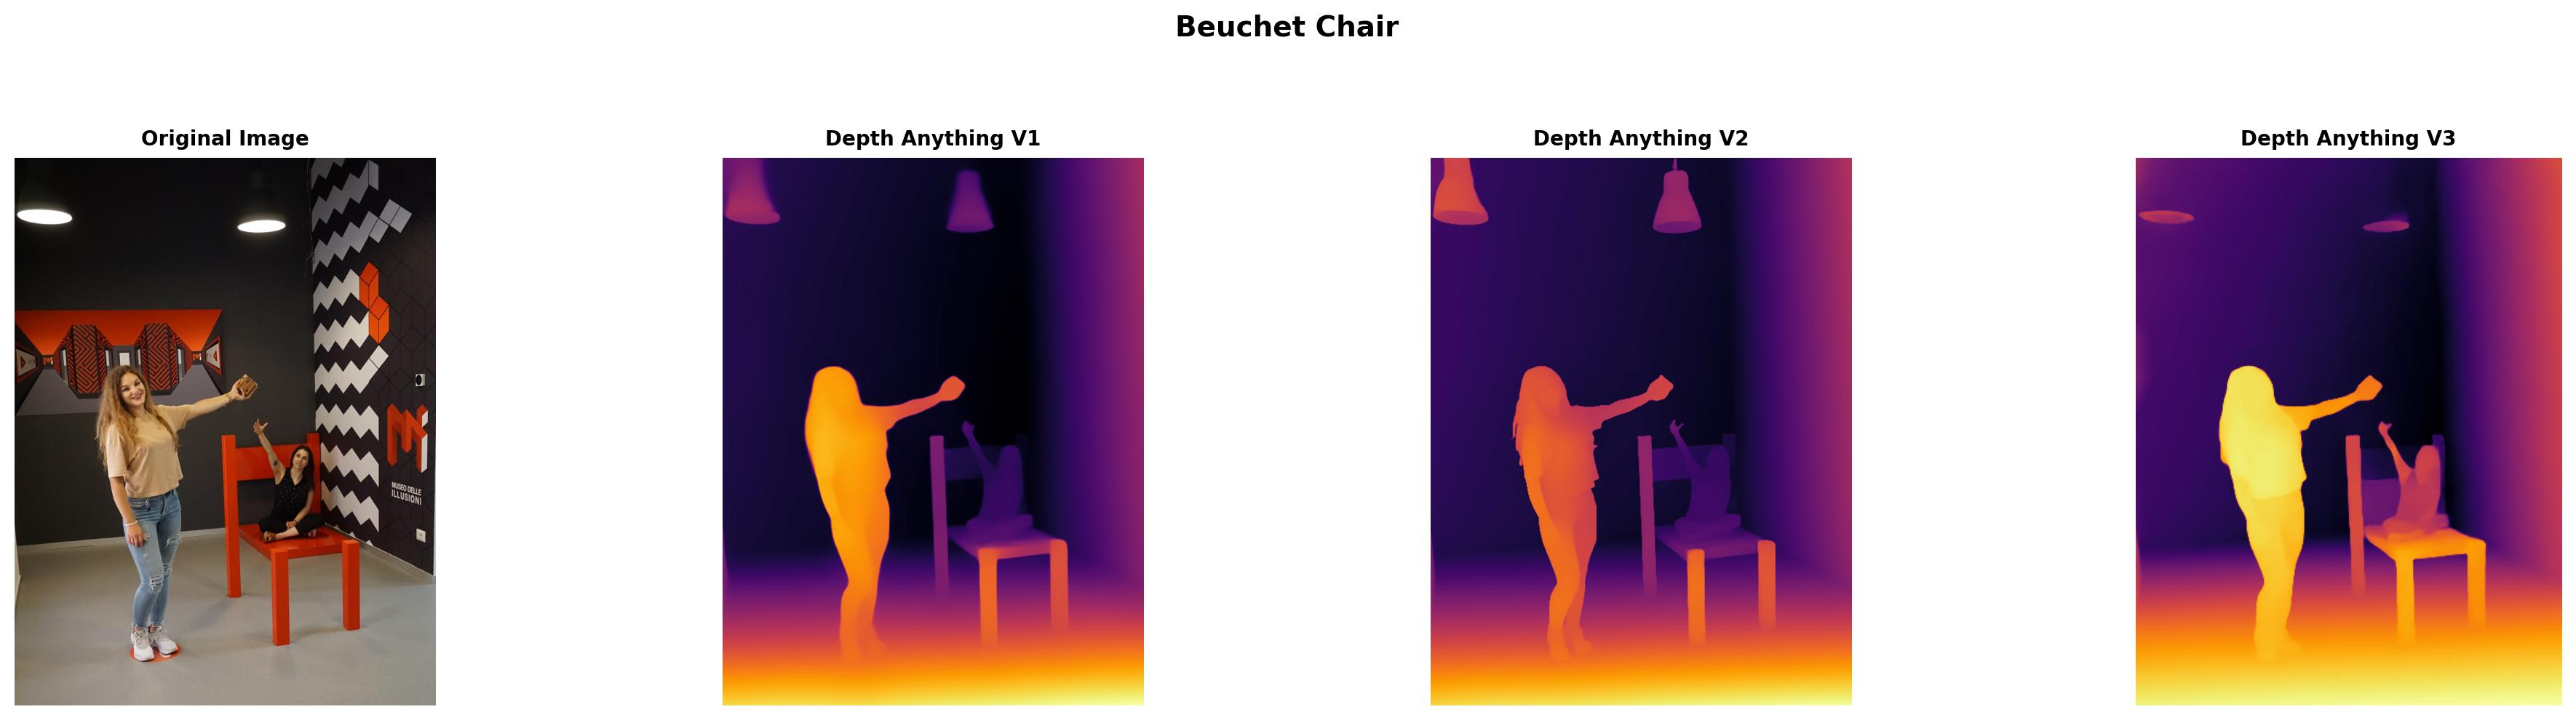
\includegraphics[width=1.05\linewidth]{figures/fig_beuchet.jpg}
  \caption{Qualitative depth maps for the Beuchet Chair illusion across Depth Anything variants (V1, V2, and V3).}
  \label{fig:Beuchet}
\end{figure}

\begin{figure}[H]
  \centering
  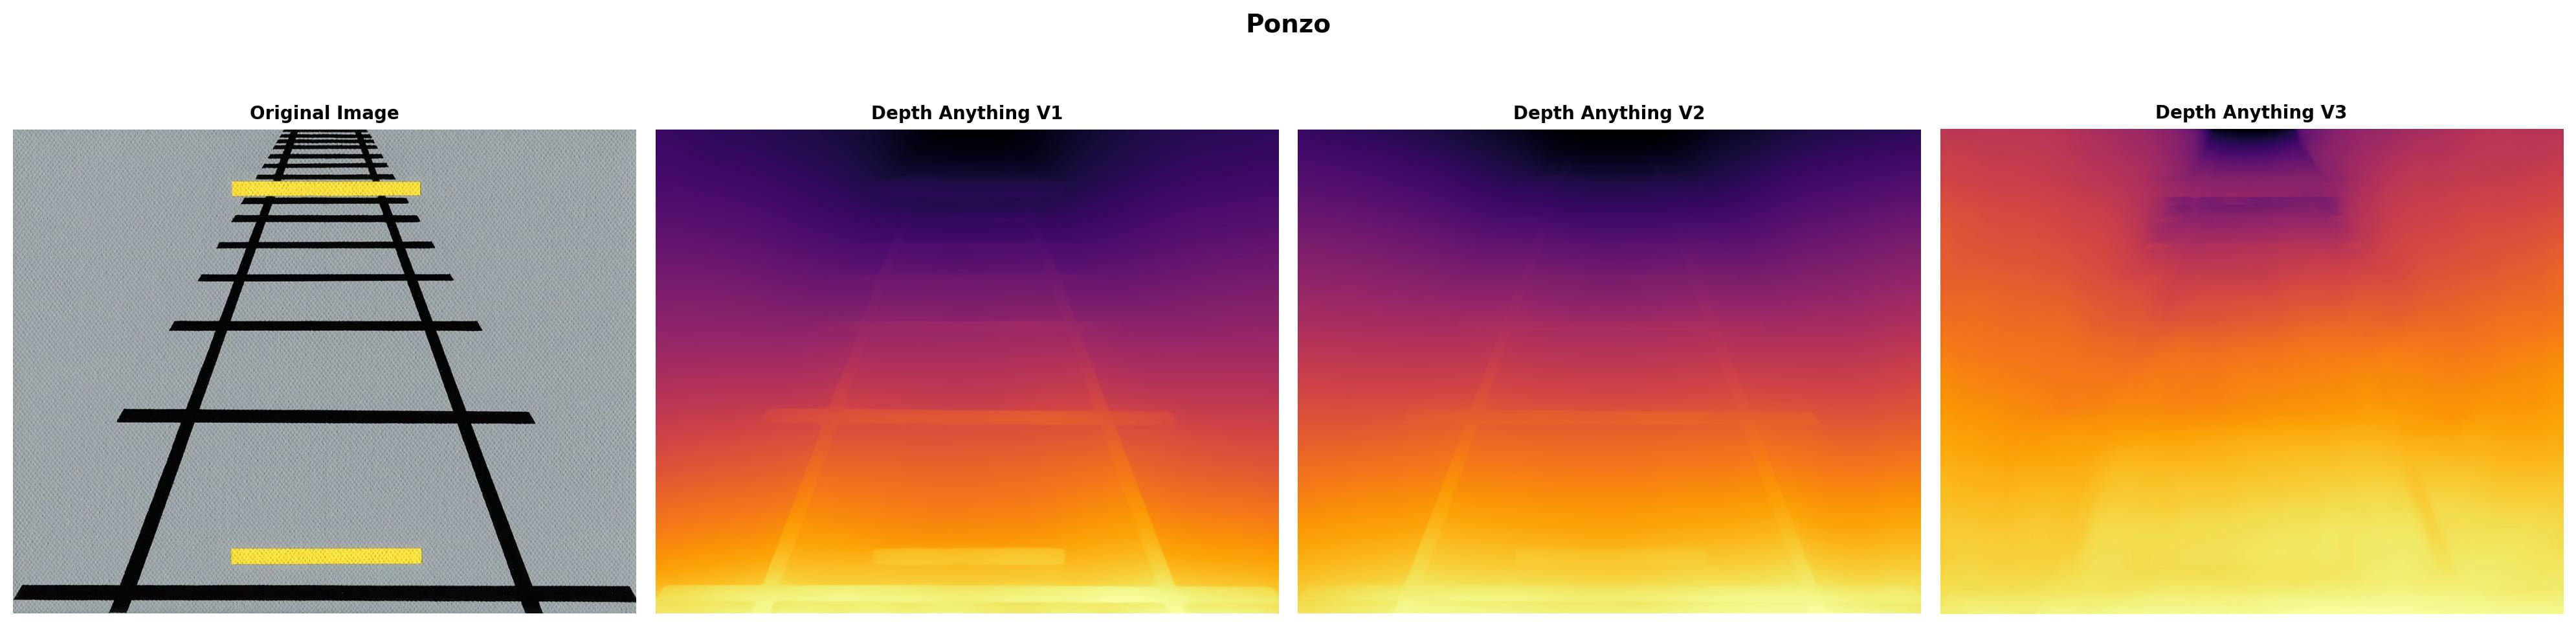
\includegraphics[width=0.95\linewidth]{figures/fig_ponzo_map.jpg}
  \caption{Qualitative depth maps for the Ponzo illusion across the Depth Anything variants. The output illustrates how the architectural priors interpret the height-in-field position of the top bar as an indicator of greater structural distance.}
  \label{fig:ponzo_map}
\end{figure}

\begin{figure}[H]
  \centering
  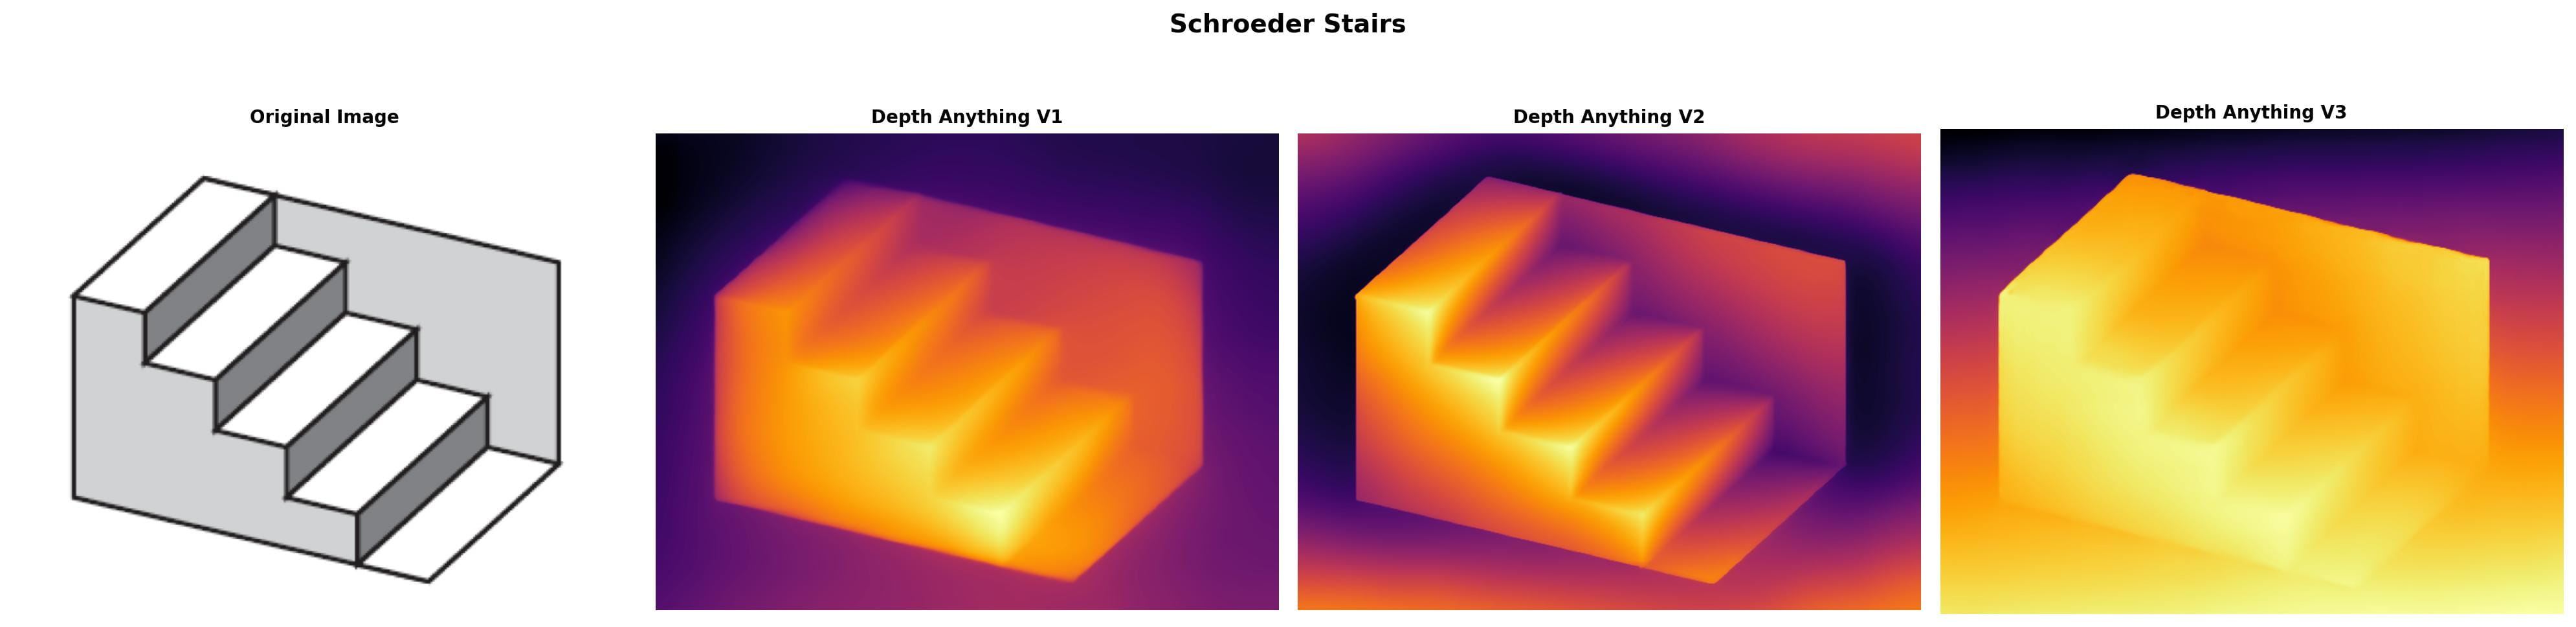
\includegraphics[width=0.95\linewidth]{figures/fig_schroeder_stairs_map.jpg}
  \caption{Qualitative depth maps for the Schröeder's Stairs illusion across the Depth Anything variants. The output documents how the model architectures resolve the bistable ambiguity by systematically converging toward the statistically dominant light-from-above interpretation.}
  \label{fig:schroeder_stairs_map}
\end{figure}

\begin{figure}[H]
  \centering
  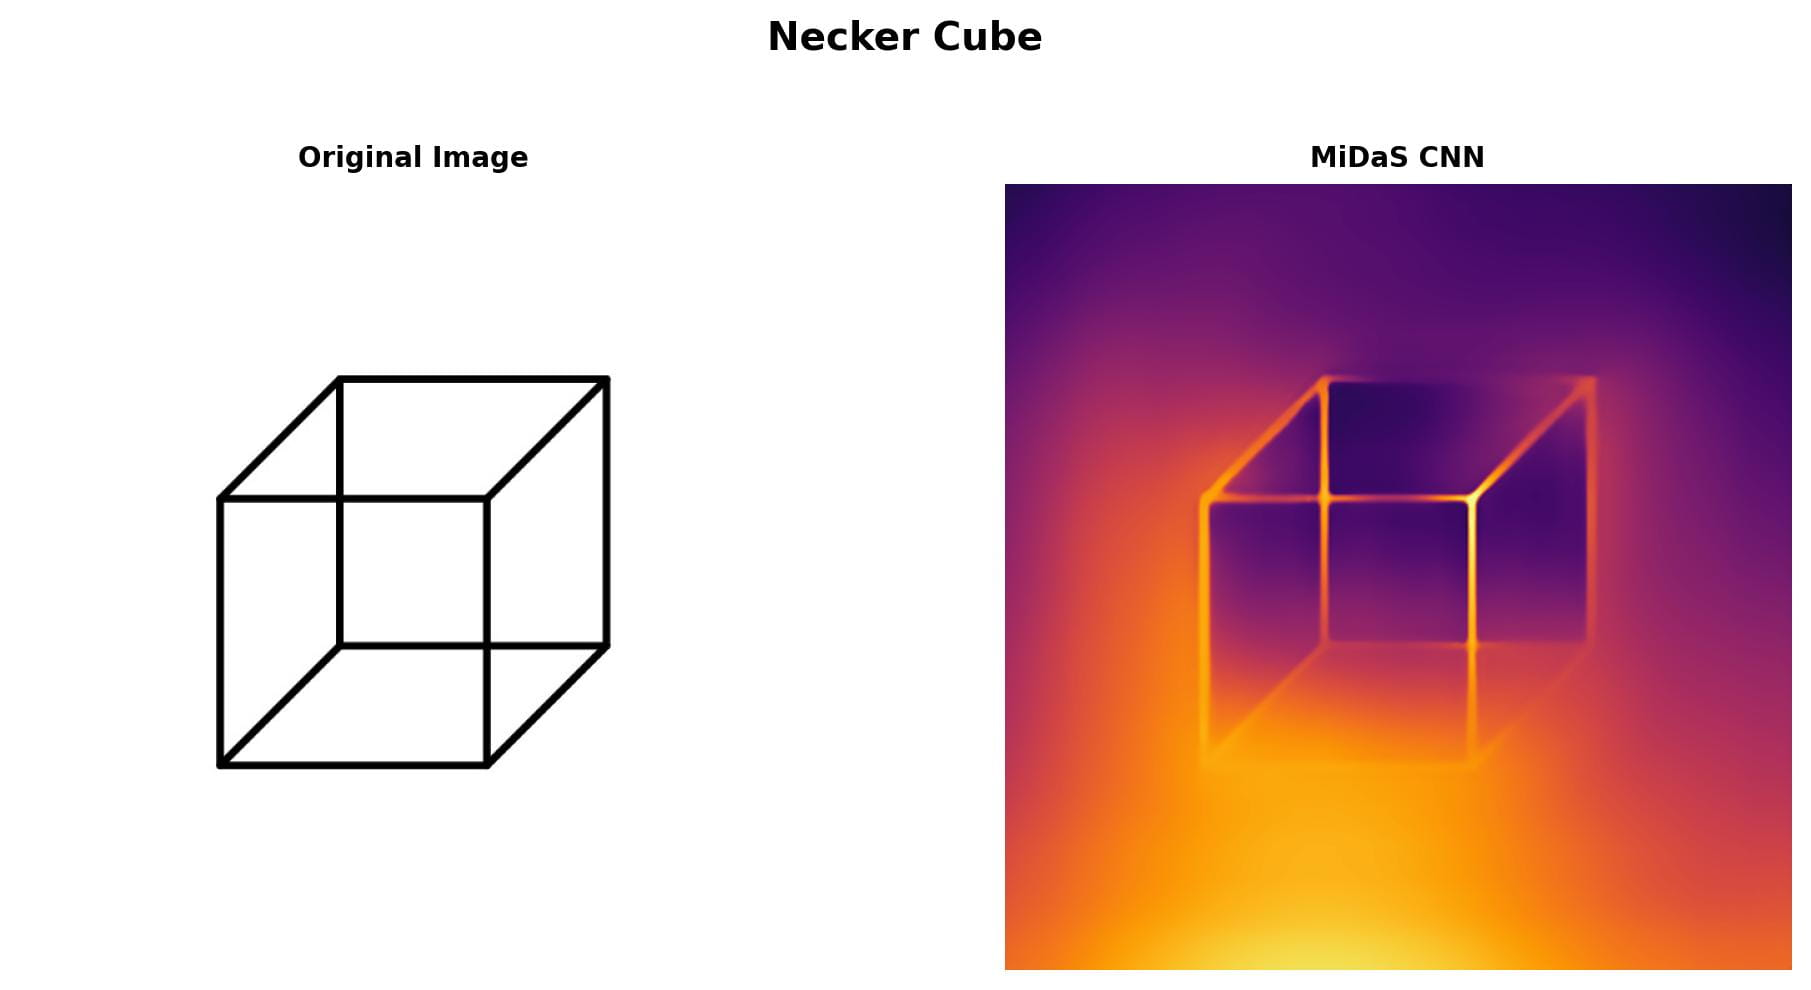
\includegraphics[width=1.02\linewidth]{figures/fig_necker_cube_midas.jpg}
  \caption{Qualitative depth map generated by MiDaS for the bistable Necker Cube stimulus. The output documents a complete non-resolution of the geometric ambiguity, as the network bypasses the 3D isometric junctions to overlay its dominant, position-dependent top-to-bottom depth gradient.}
  \label{fig:necker_cube_midas}
\end{figure}

% 1. Anamorphic Cube
\begin{figure}[H]
  \centering
  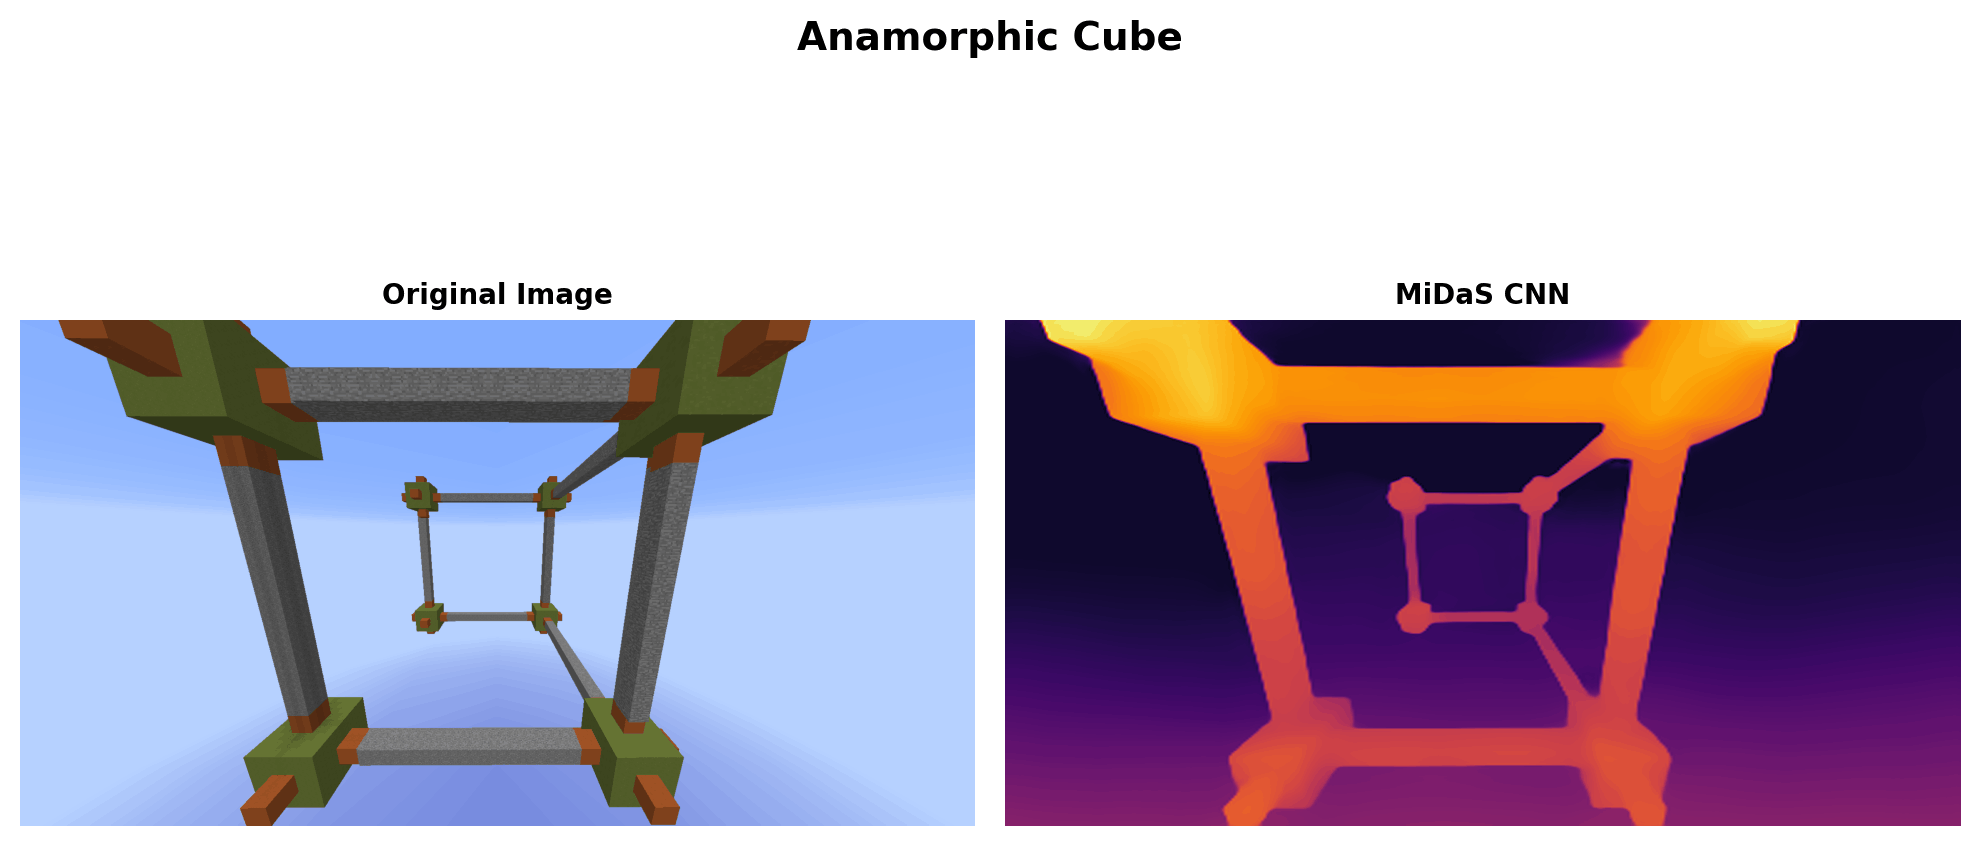
\includegraphics[width=\linewidth]{figures/fig_anamorphic_cube.png}
  \caption{Cross-domain validation of the Anamorphic Cube experiment under MiDaS. The depth map highlights the network's structural resistance to context-driven forced-perspective tricks, successfully bypassing the illusory multi-object alignment to decode the true disjoint geometry.}
  \label{fig:fig_anamorphic_cube}
\end{figure}

% 2. Fake Block
\begin{figure}[H]
  \centering
  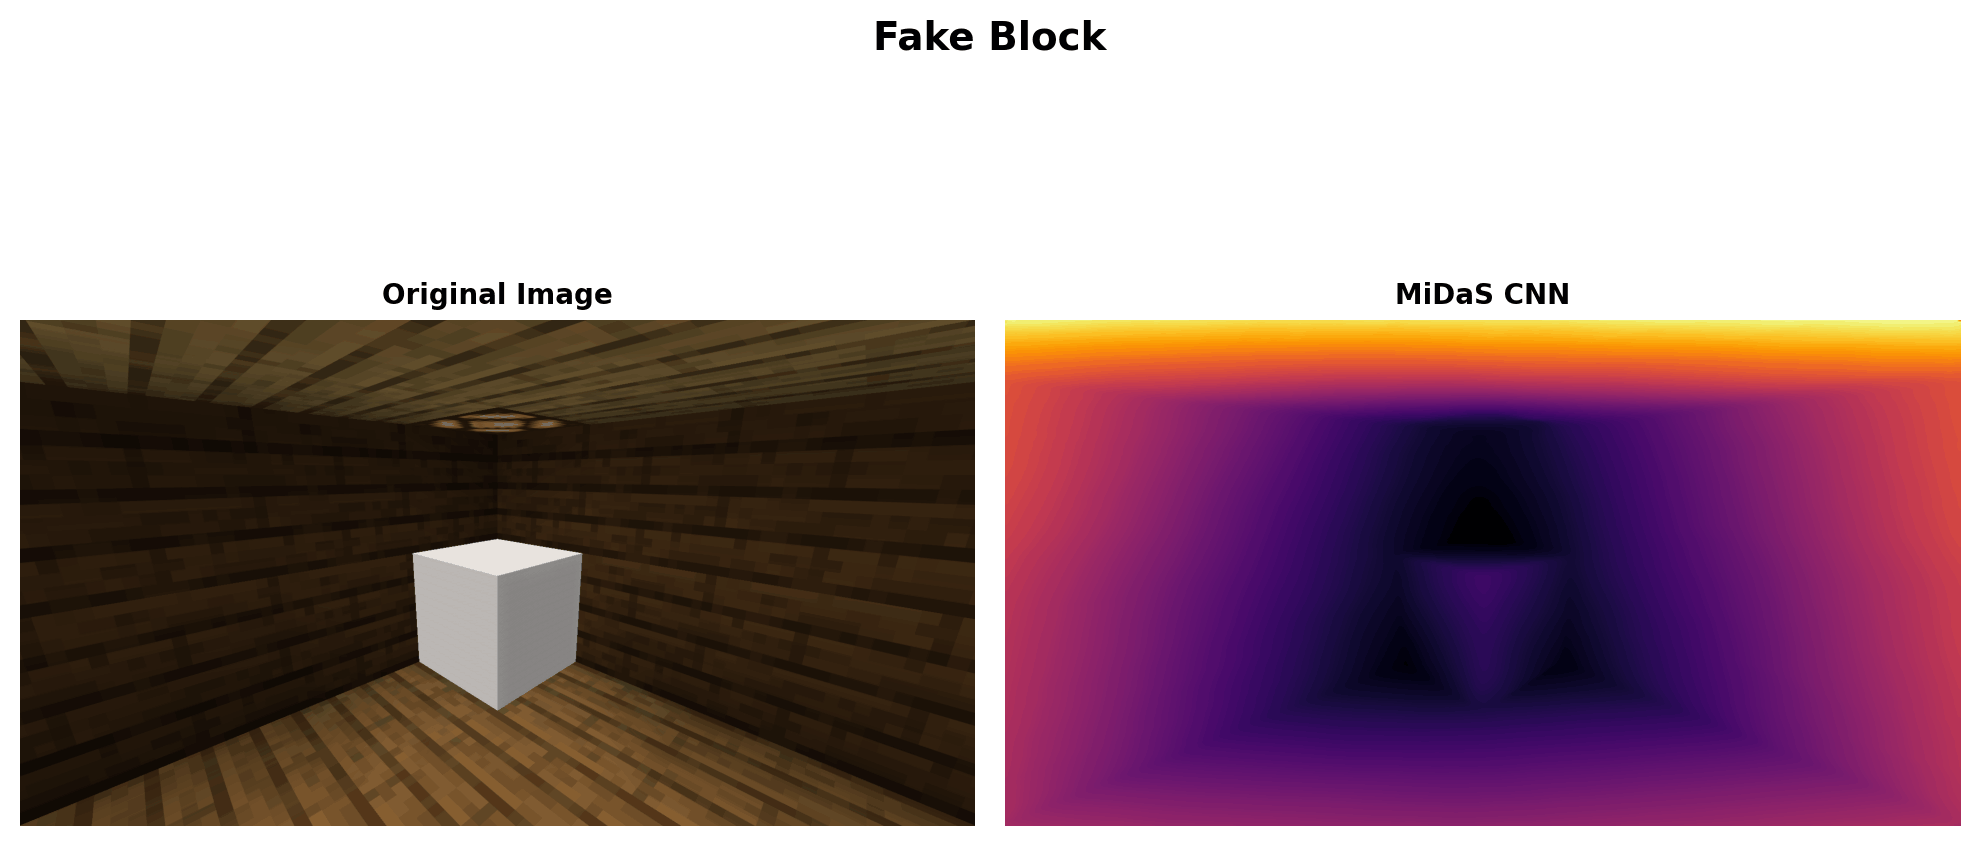
\includegraphics[width=\linewidth]{figures/fig_fake_block.png}
  \caption{Cross-domain validation of the Fake Block stimulus processed by MiDaS. Reflecting a low average contextual sensitivity ($\Delta I = 7.9$ for forced perspective), the output confirms that the model's resistance to scale anomalies is an architecture-level property preserved under domain shifts.}
  \label{fig:fig_fake_block}
\end{figure}

% 3. Depth Incongruence
\begin{figure}[H]
  \centering
  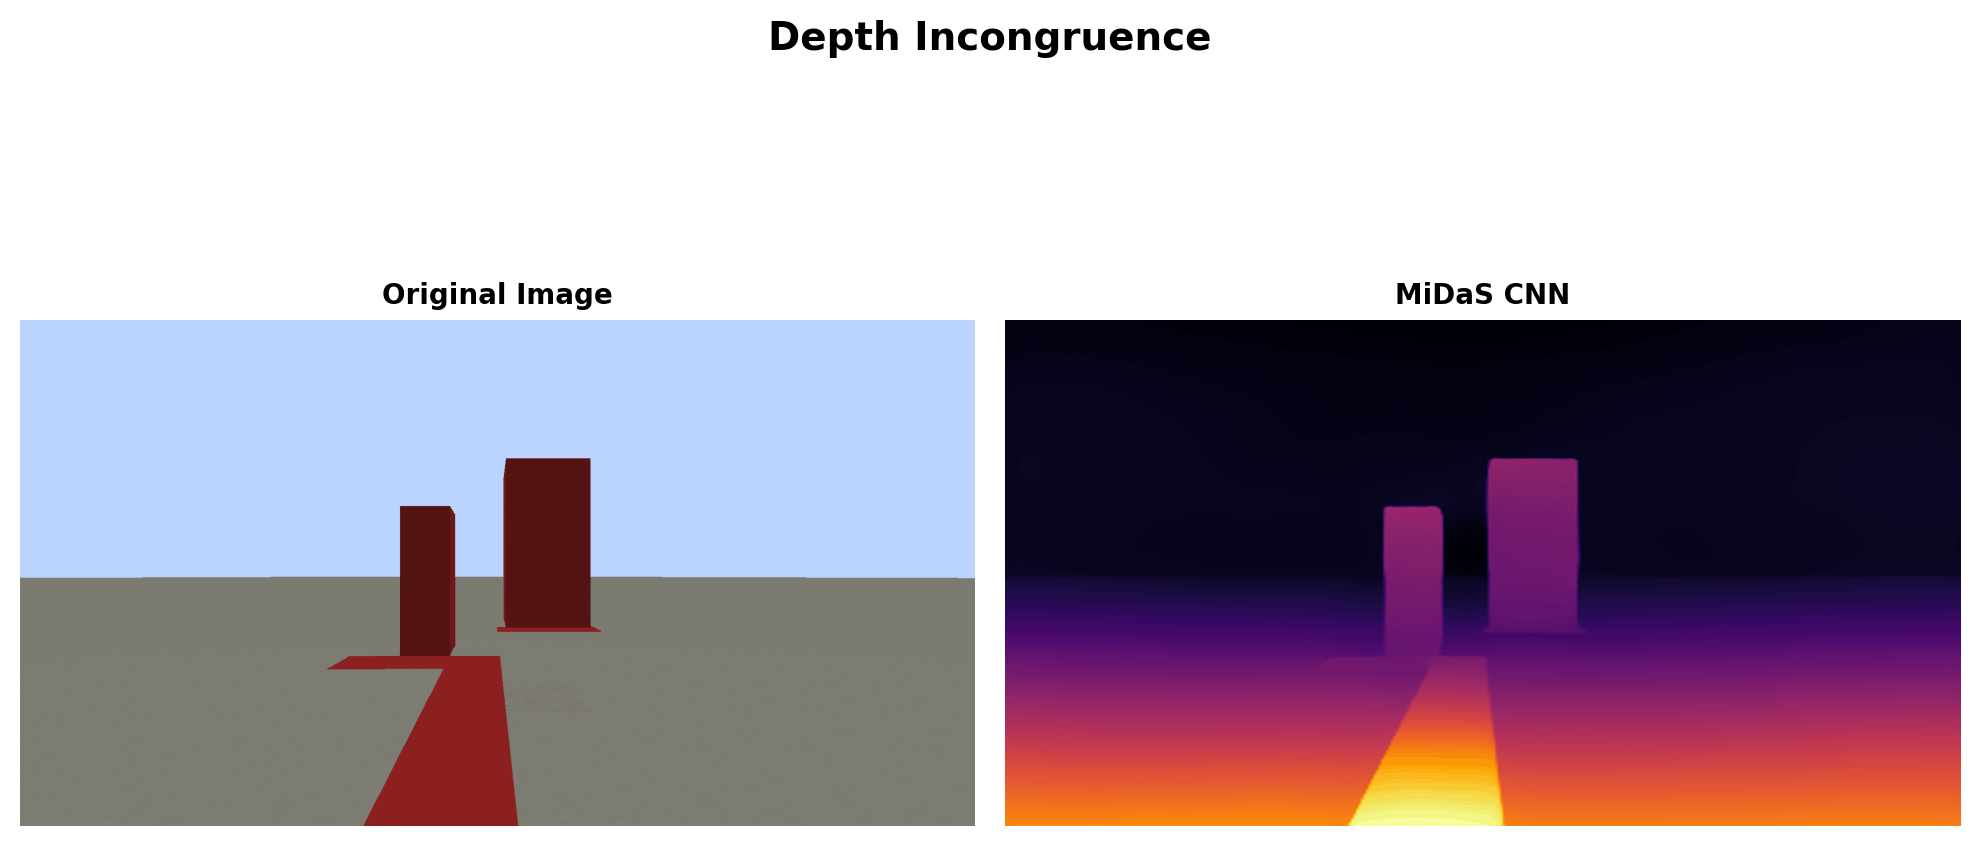
\includegraphics[width=\linewidth]{figures/fig_depth_incongruence.png}
  \caption{Cross-domain validation of the Depth Incongruence experiment under MiDaS. The resulting depth map captures the model's inherent resistance to perspective context, failing to be deceived by the size-distance manipulation and relies instead on its rigid vertical mapping.}
  \label{fig:fig_depth_incongruence}
\end{figure}

\subsubsection*{C. Quantitative Psychophysical Experiments visualizations.}
\label{app:psychophysics_curves}
\textbf{Psychophysical Response Profiles.} This subsection aggregates the complete set of behavioral curves tracking the depth delta ($\Delta I = \text{Target} - \text{Context}$) across the incremental 30-frame stimulus evolution sequences. These plots isolate the precise boundaries where each model family shifts its perceptual ordering, defining the empirical foundation for the reported PSE and JND thresholds.

\begin{figure}[H]
  \centering
  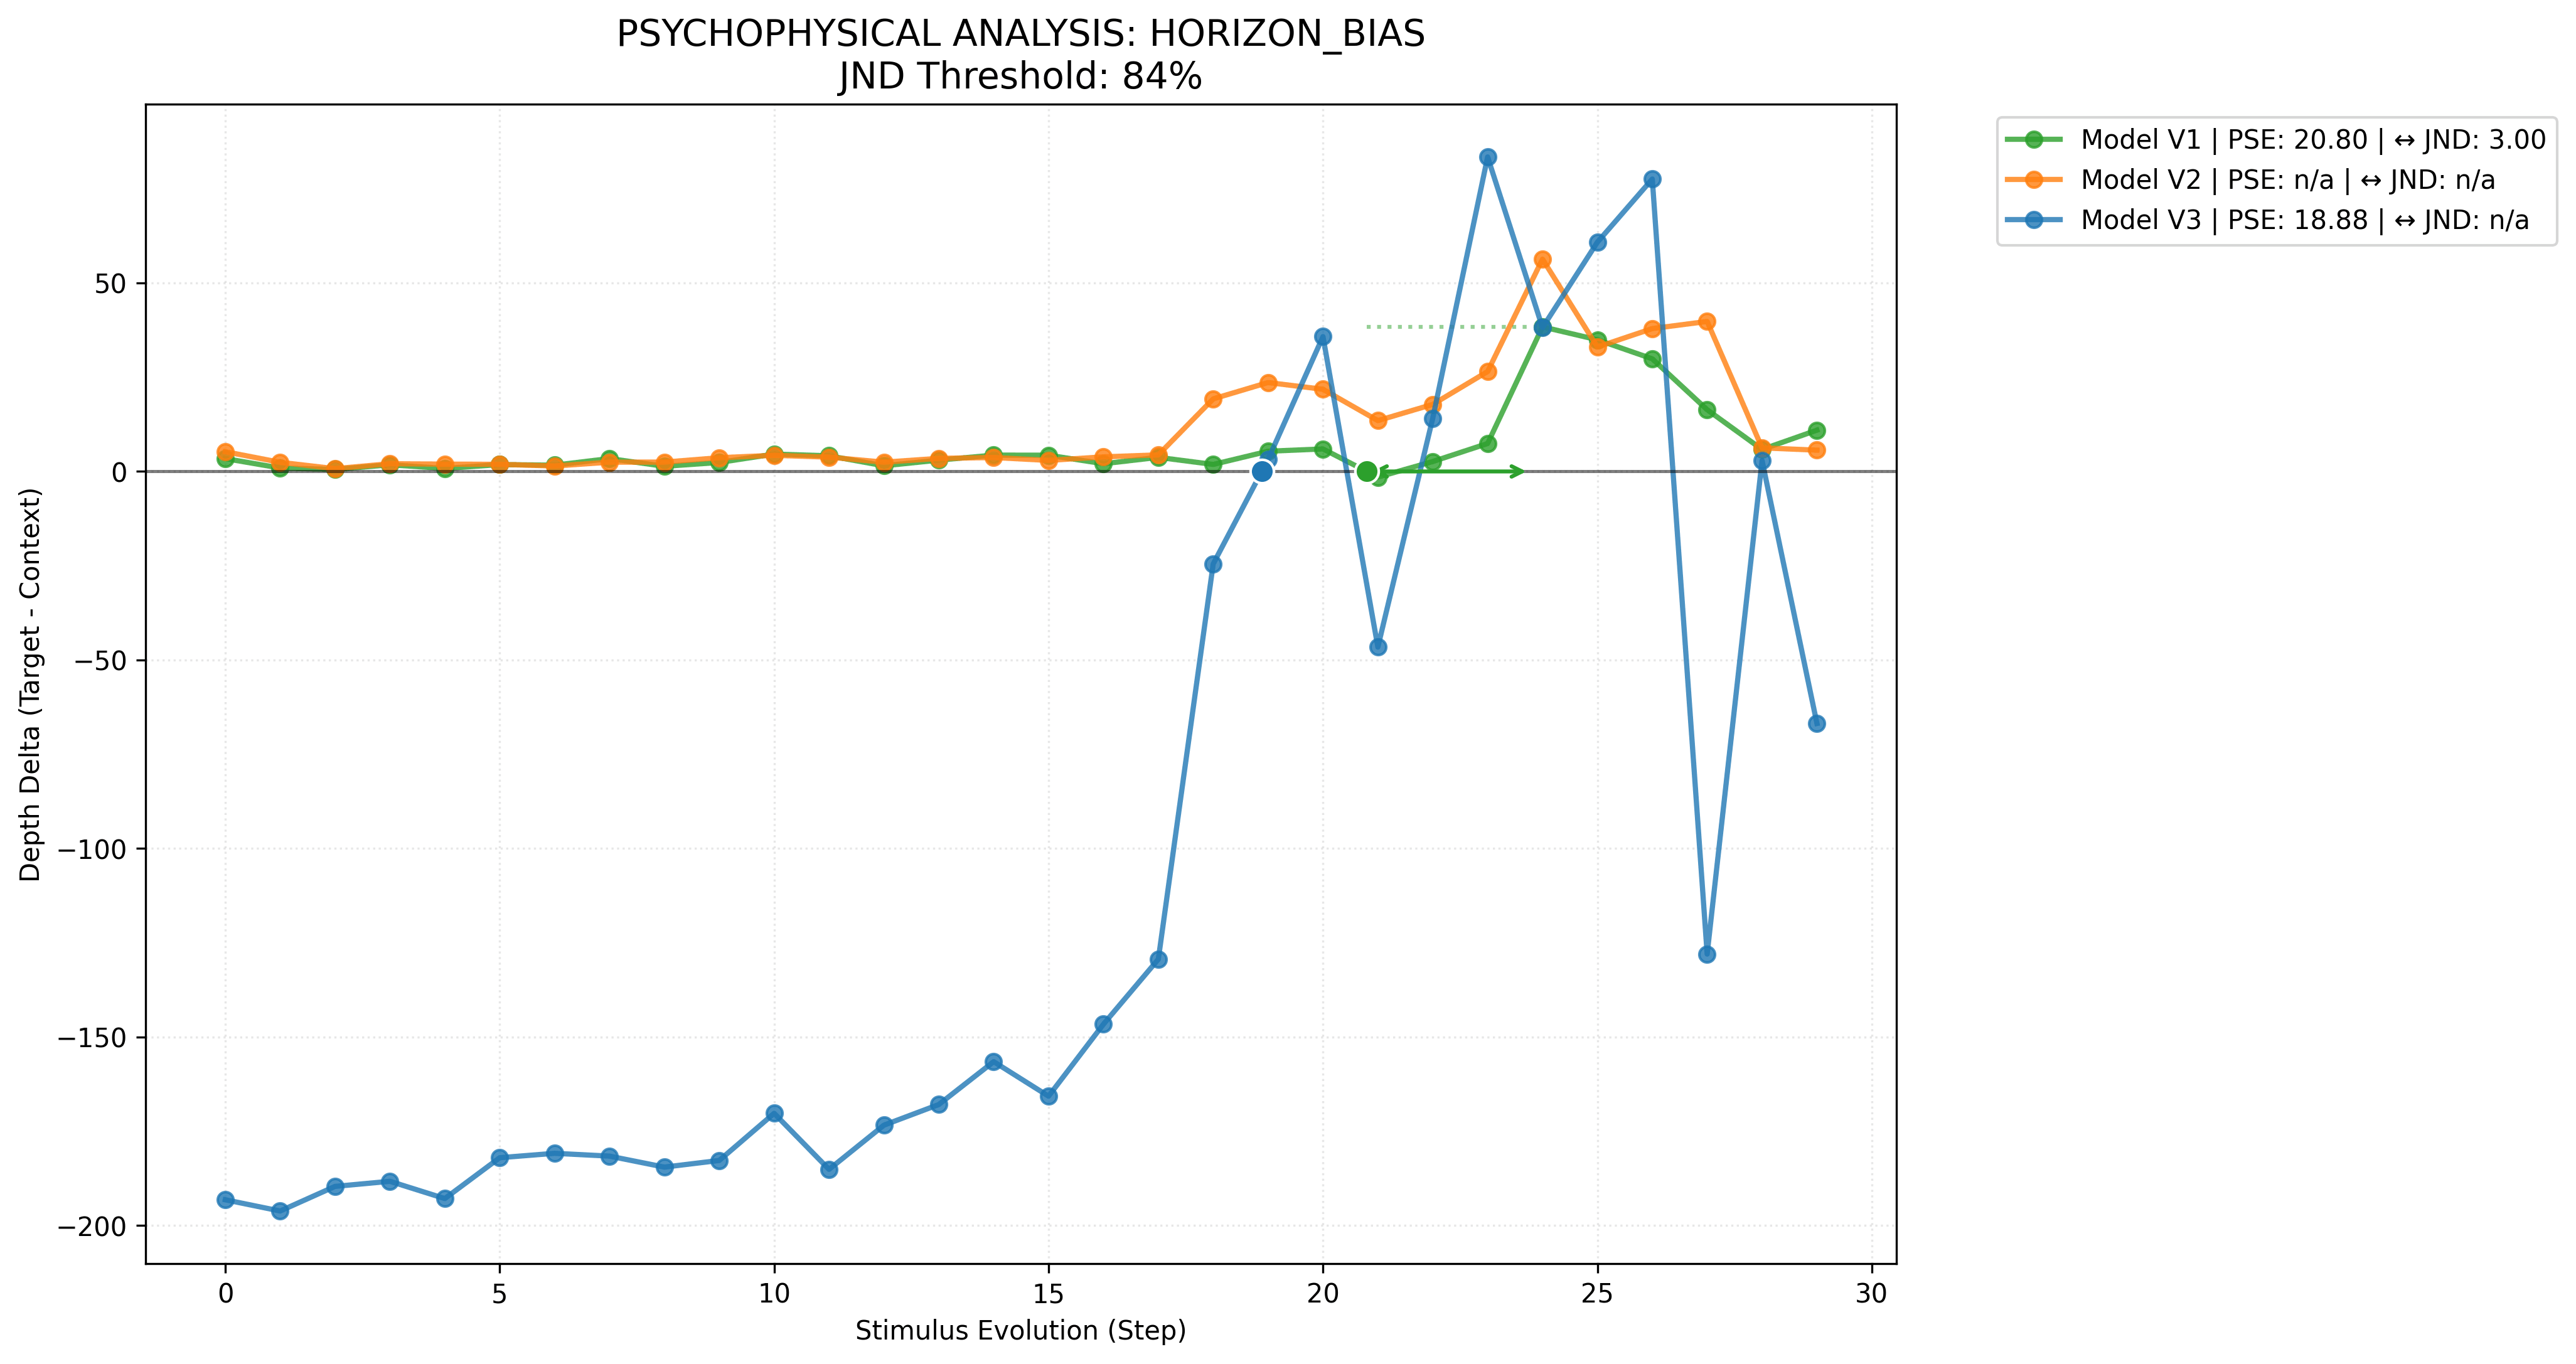
\includegraphics[width=1.02\linewidth]{figures/fig_horizon_bias.png}
  \caption{Psychophysical analysis of the Horizon bias. The plot tracks the depth delta across the 30-step stimulus evolution, contrastingly showcasing V1's smooth adaptation, V2's rigid, strictly positive horizon-driven spatial prior, and the high localized variability exhibited by V3.}
  \label{fig:horizon_bias}
\end{figure}

% 3. Relative Size Bias
\begin{figure}[H]
  \centering
  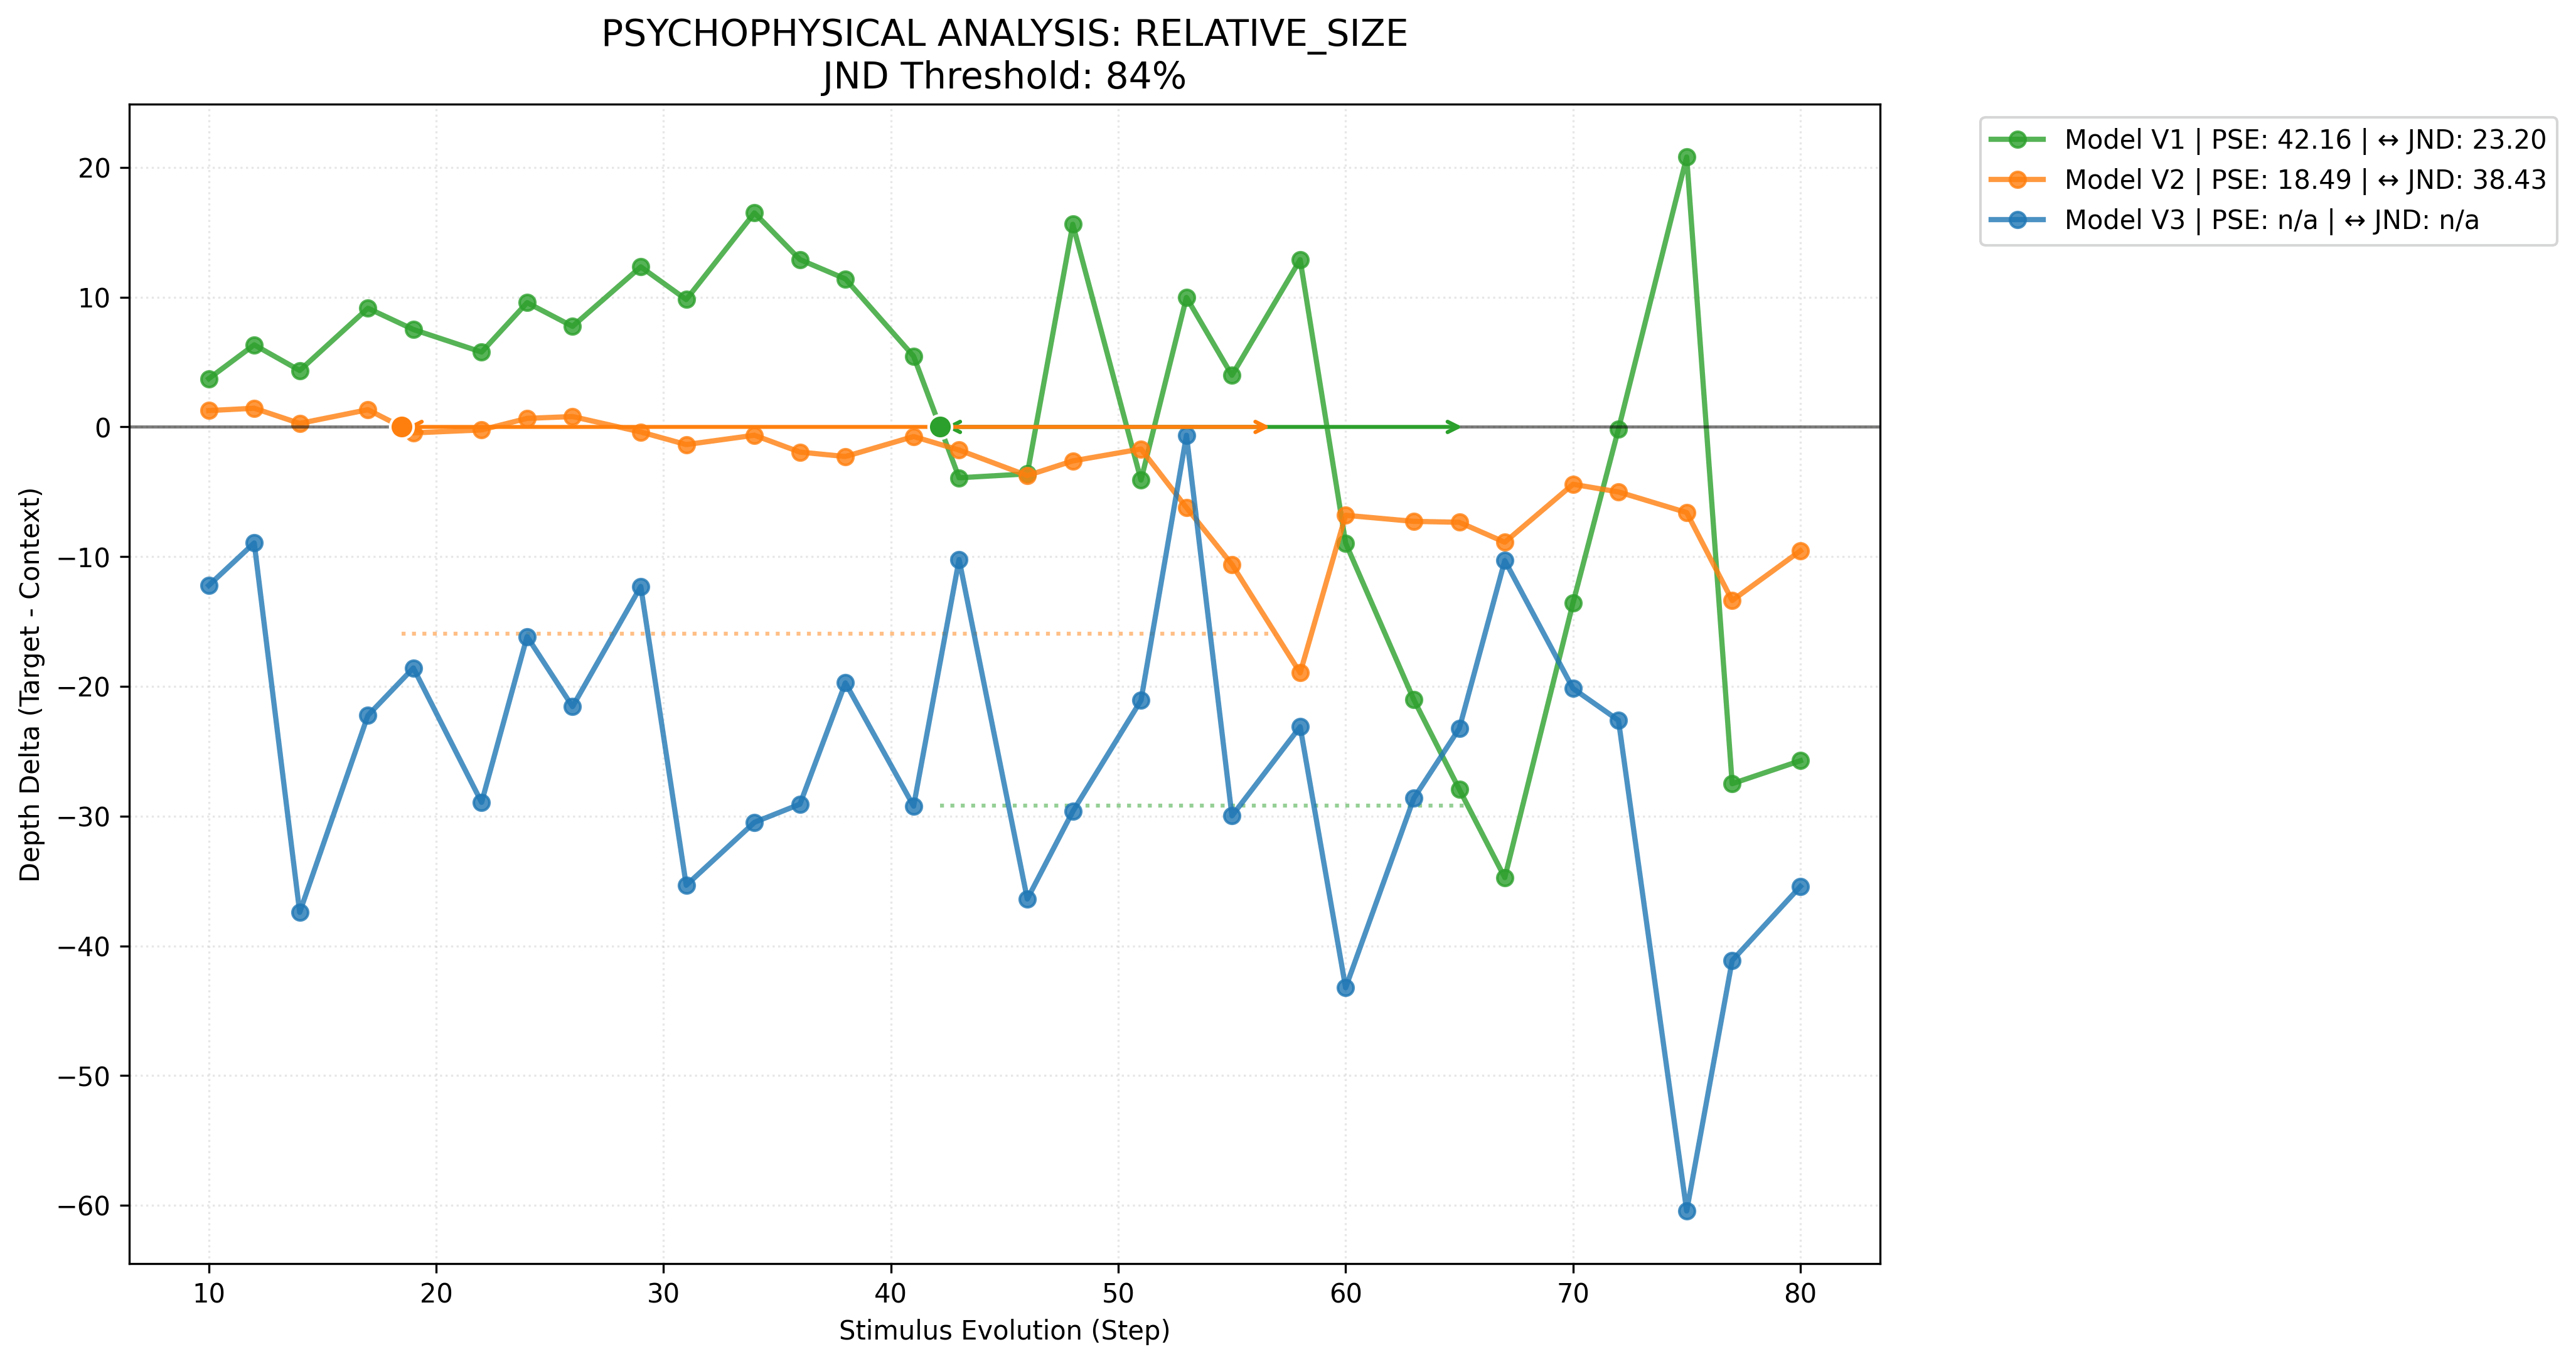
\includegraphics[width=1.02\linewidth]{figures/fig_relative_size_bias.png}
  \caption{Psychophysical analysis of the Relative Size bias. The plot tracks the evolution of depth delta, mapping the wider transition window required by V2 ($JND \approx 1.7\times$ larger than V1) and the unyielding negative depth ordering maintained by V3 across the entire stimulus range.}
  \label{fig:relative_size_bias}
\end{figure}

% 4. Texture Gradient Bias
\begin{figure}[H]
  \centering
  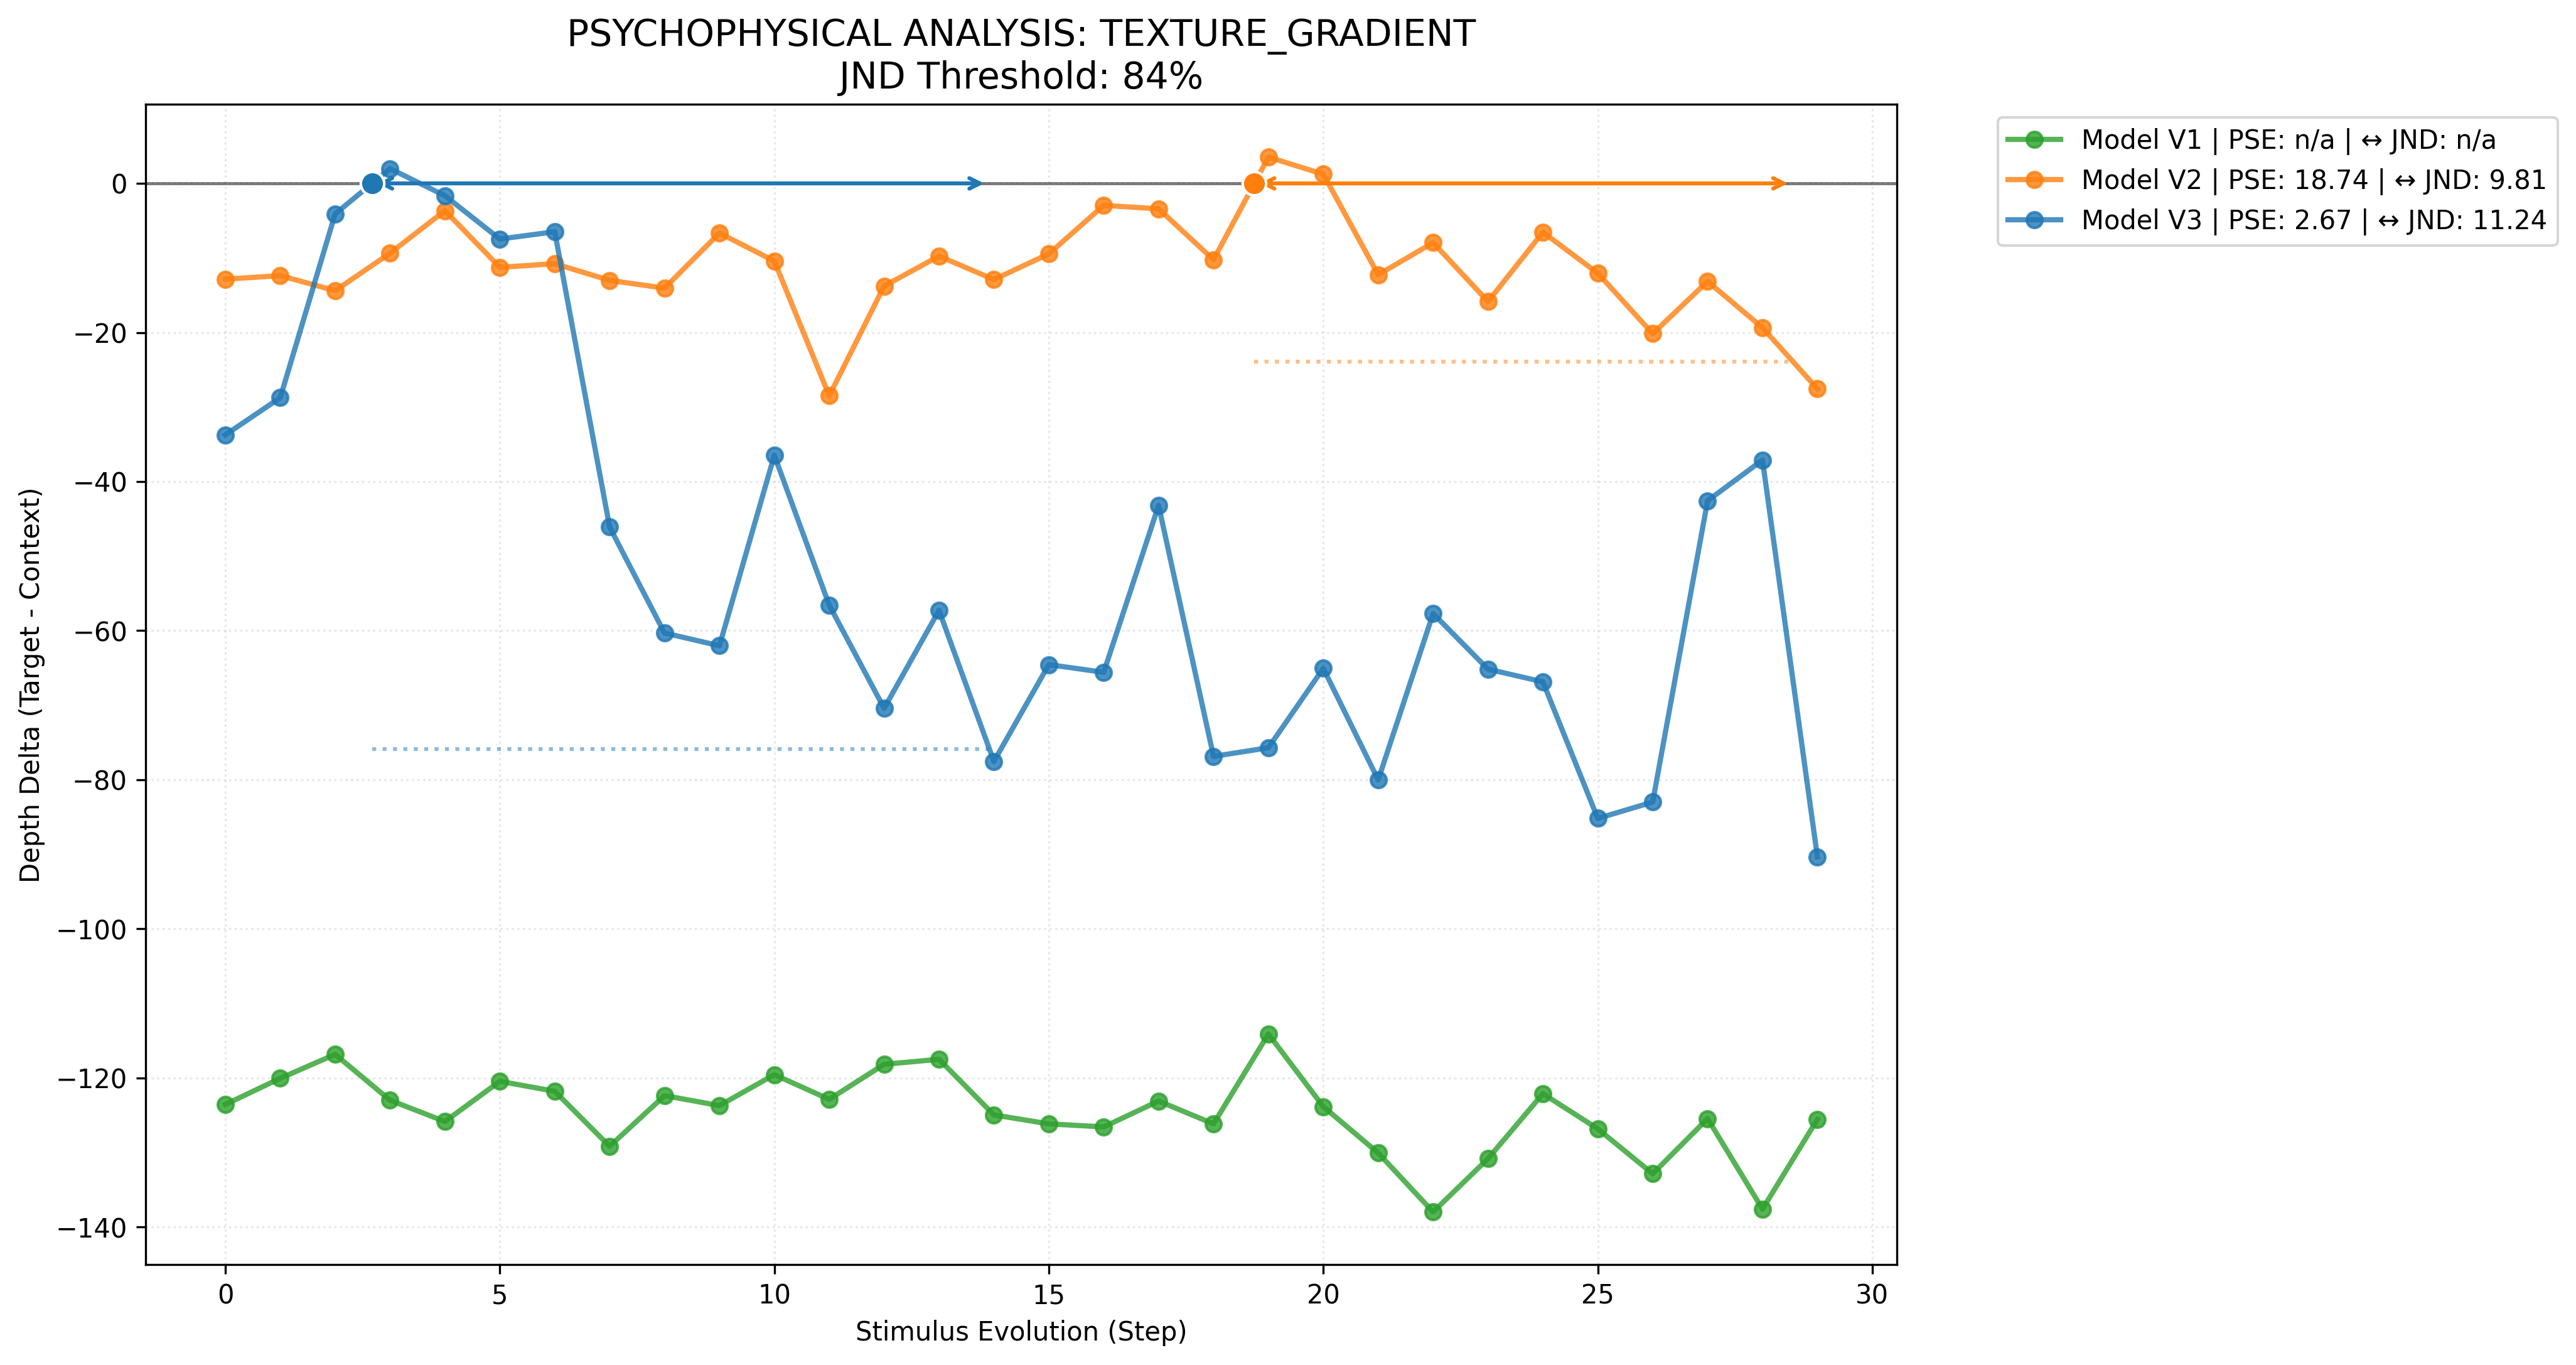
\includegraphics[width=1.02\linewidth]{figures/fig_texture_gradient_bias.png}
  \caption{Psychophysical analysis of the Texture Gradient bias. The curves contrast V1's rigid, single-sided response against the broadly convergent behavioral responses of the later architectures (V2 and V3), which successfully capture density shifts as active depth cues.}
  \label{fig:texture_gradient_bias}
\end{figure}

% 5. Blur Bias
\begin{figure}[H]
  \centering
  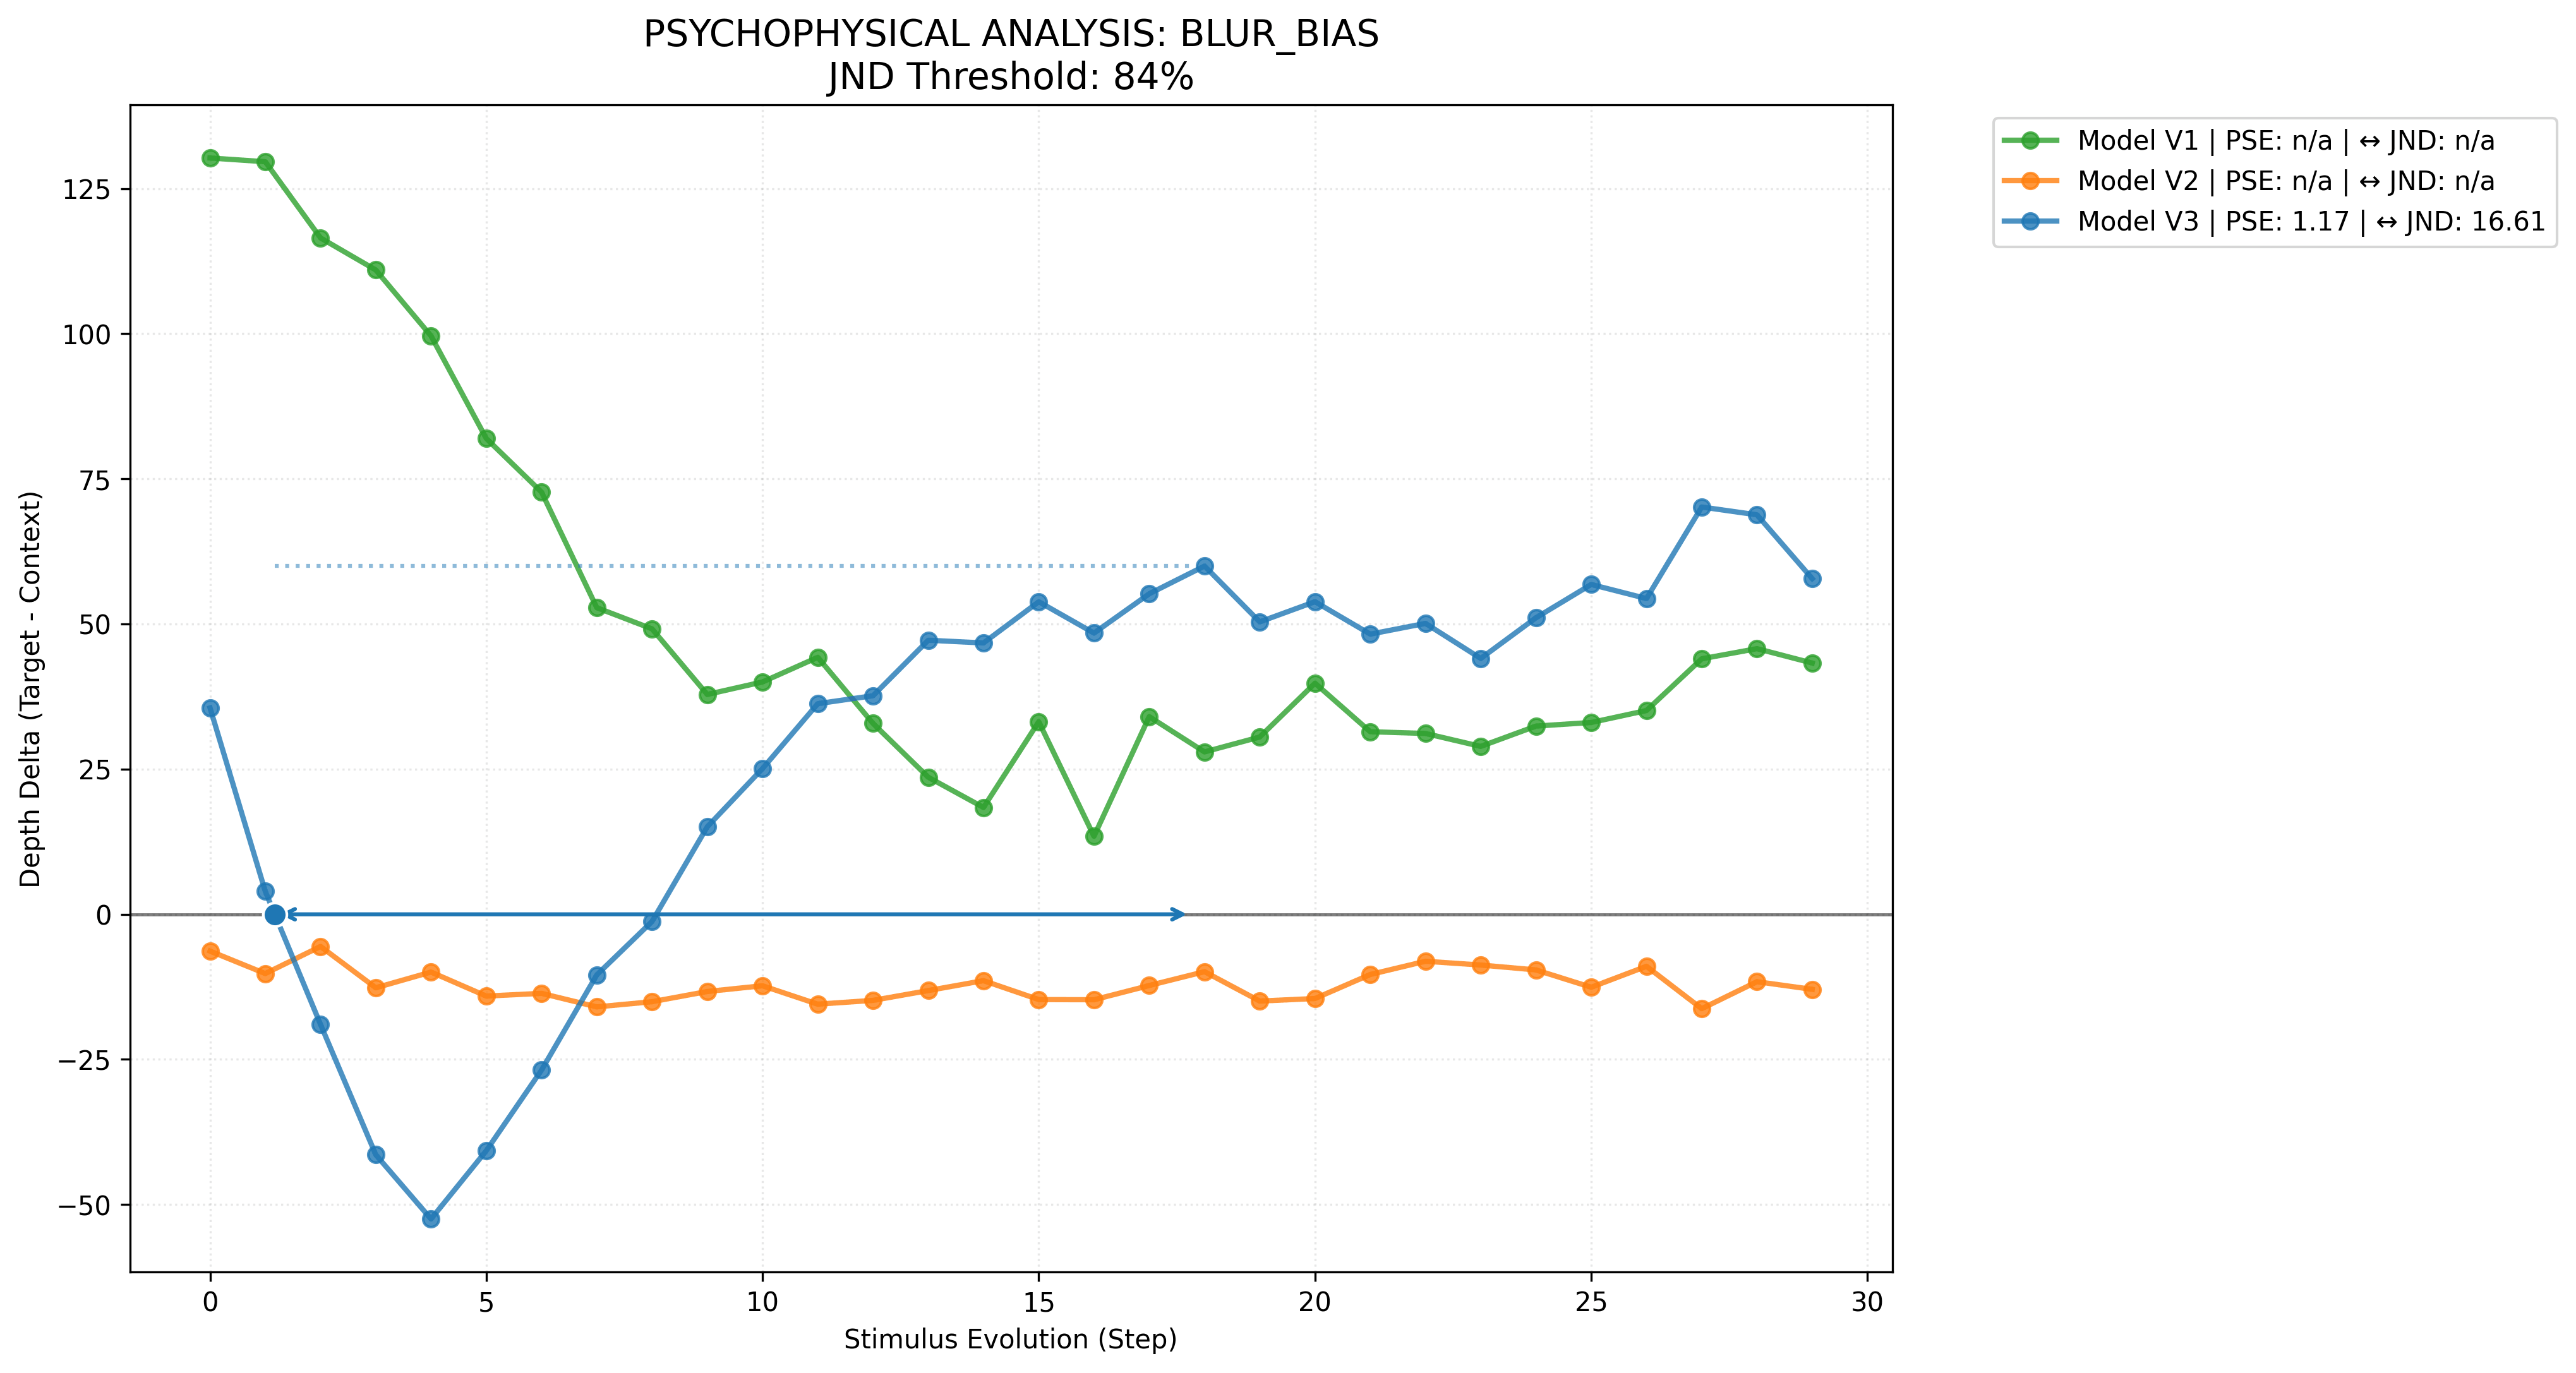
\includegraphics[width=1.02\linewidth]{figures/fig_blur_bias.png}
  \caption{Psychophysical analysis of the Blur bias. The plot highlights a definitive architectural divergence where V1 and V2 remain locked in opposite signed regimes, isolating V3 as the unique architecture capable of resolving a clear subjective equality point ($PSE = 1.17$).}
  \label{fig:blur_bias}
\end{figure}

% 6. Aerial Perspective Bias
\begin{figure}[H]
  \centering
  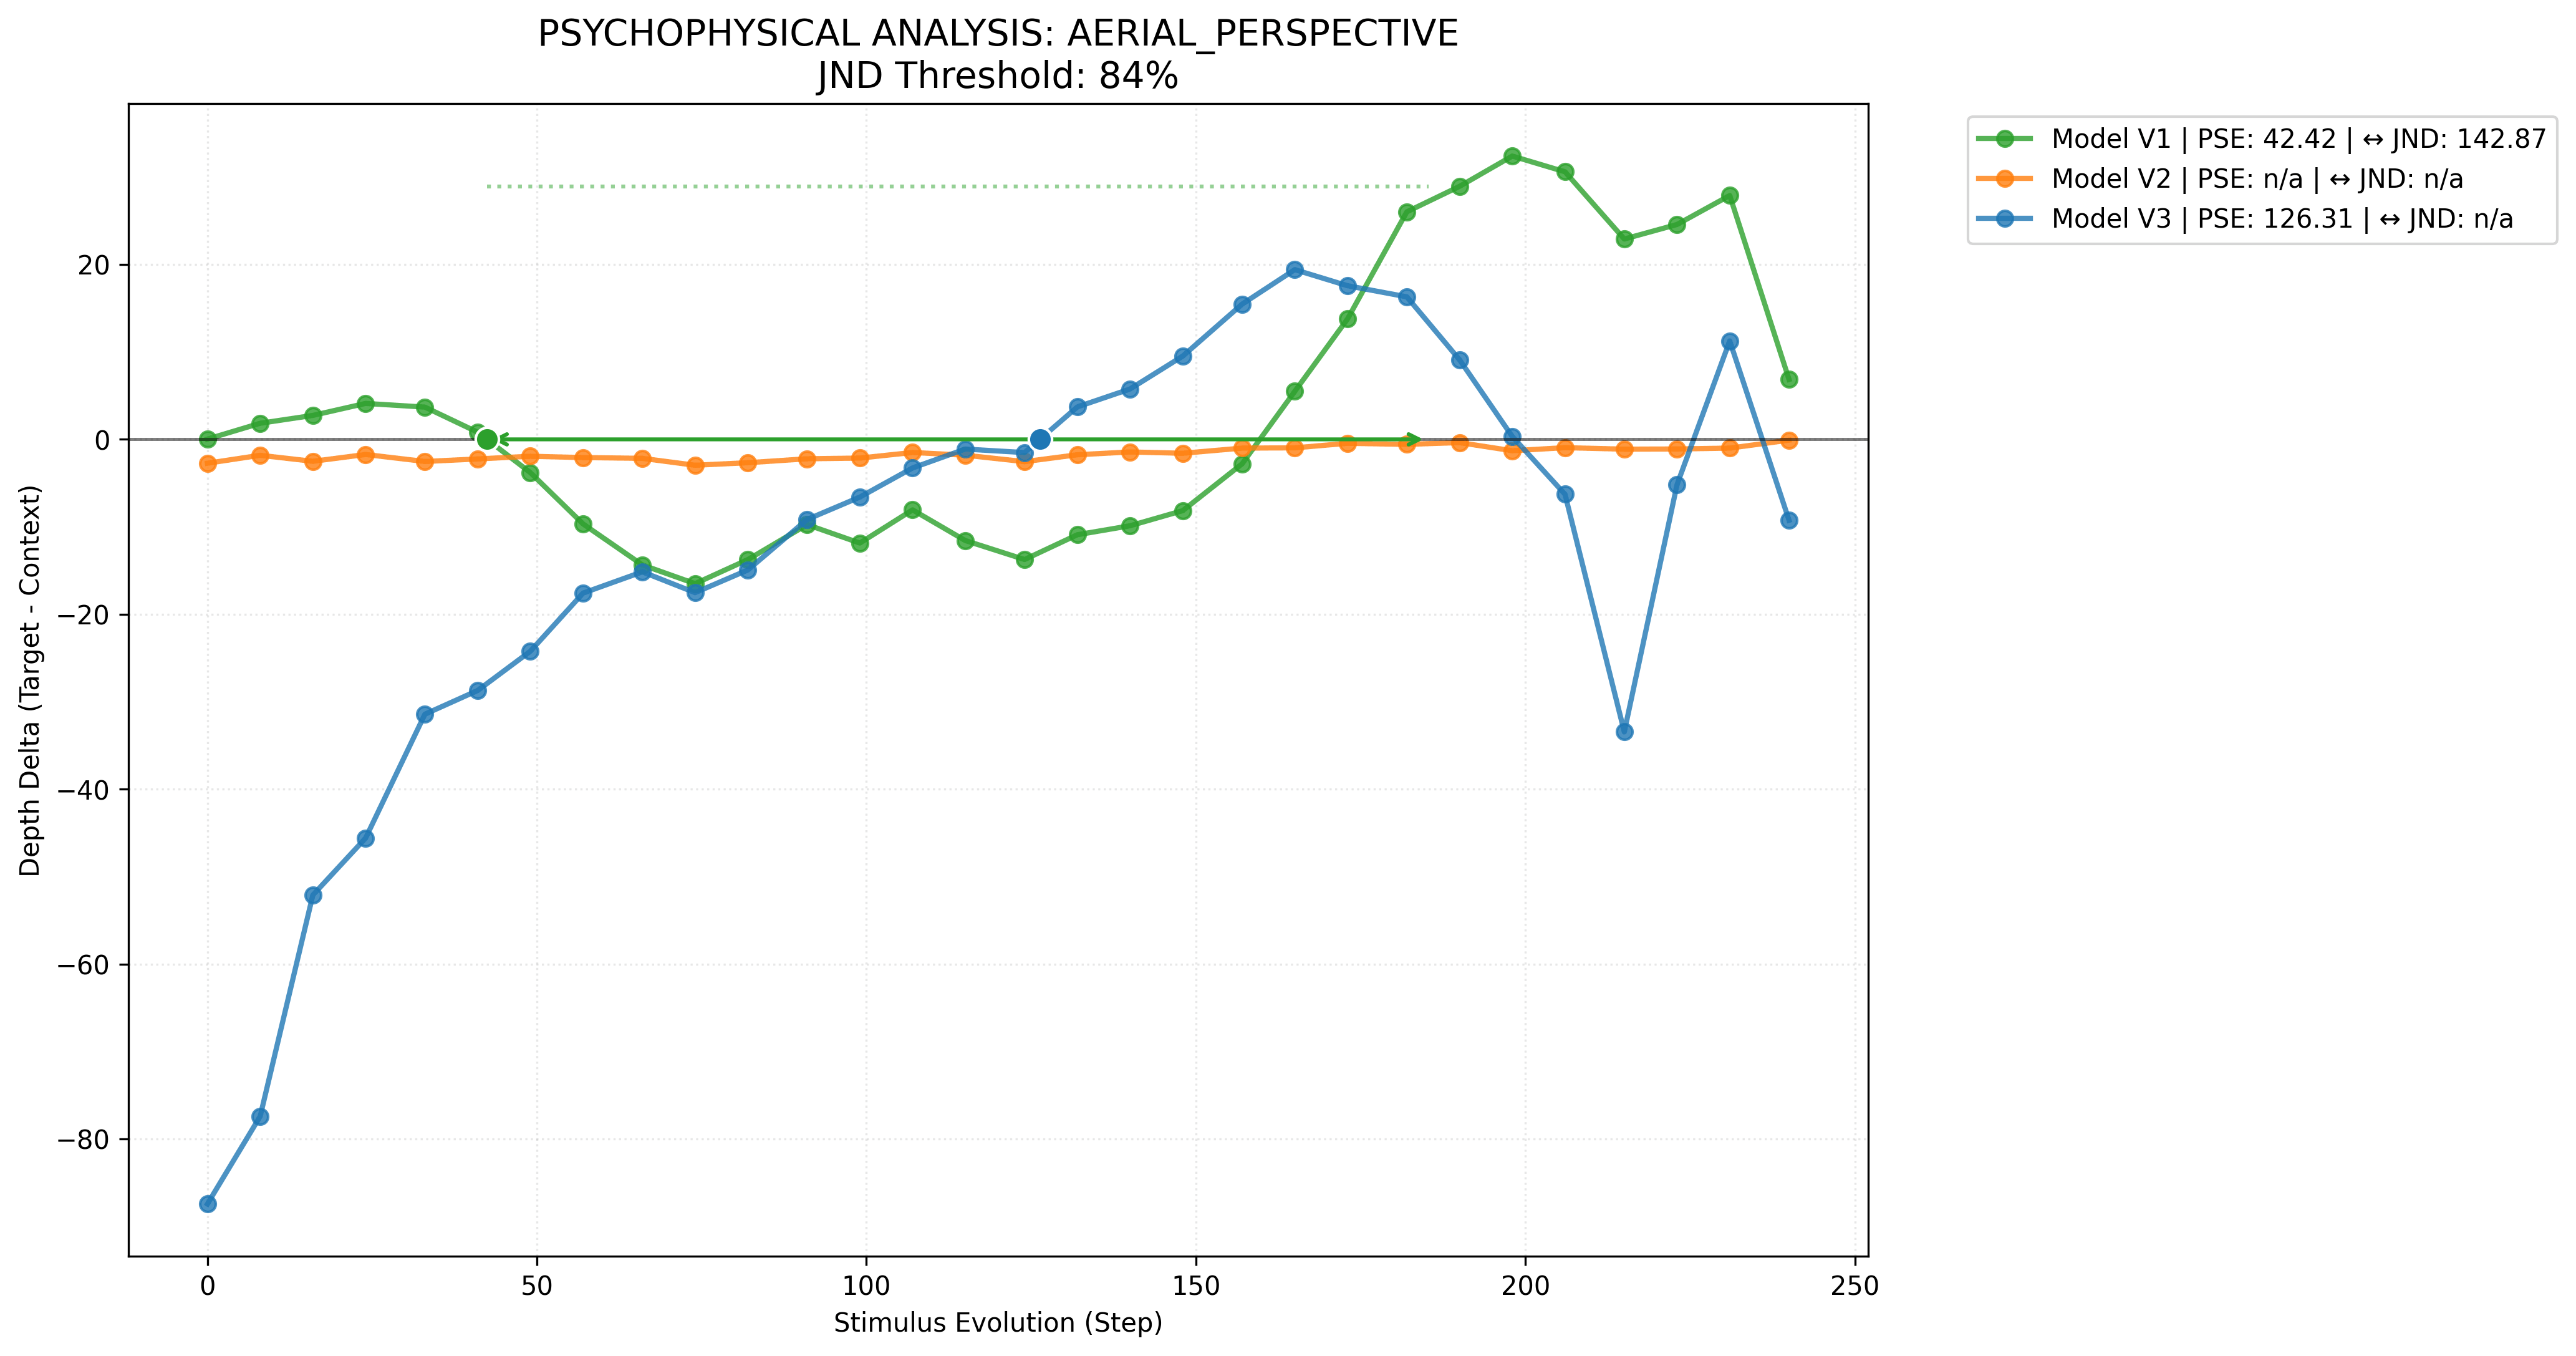
\includegraphics[width=1.02\linewidth]{figures/fig_aerial_perspective_bias.png}
  \caption{Psychophysical analysis of the Aerial Perspective bias. The response profiles showcase a shallow, high-variance transition for V1, an insensitive, near-zero trajectory for V2 under contrast decay, and a late, characteristically noisy perceptual shift for V3.}
  \label{fig:aerial_perspective_bias}
\end{figure}

% 7. Shading Bias
\begin{figure}[H]
  \centering
  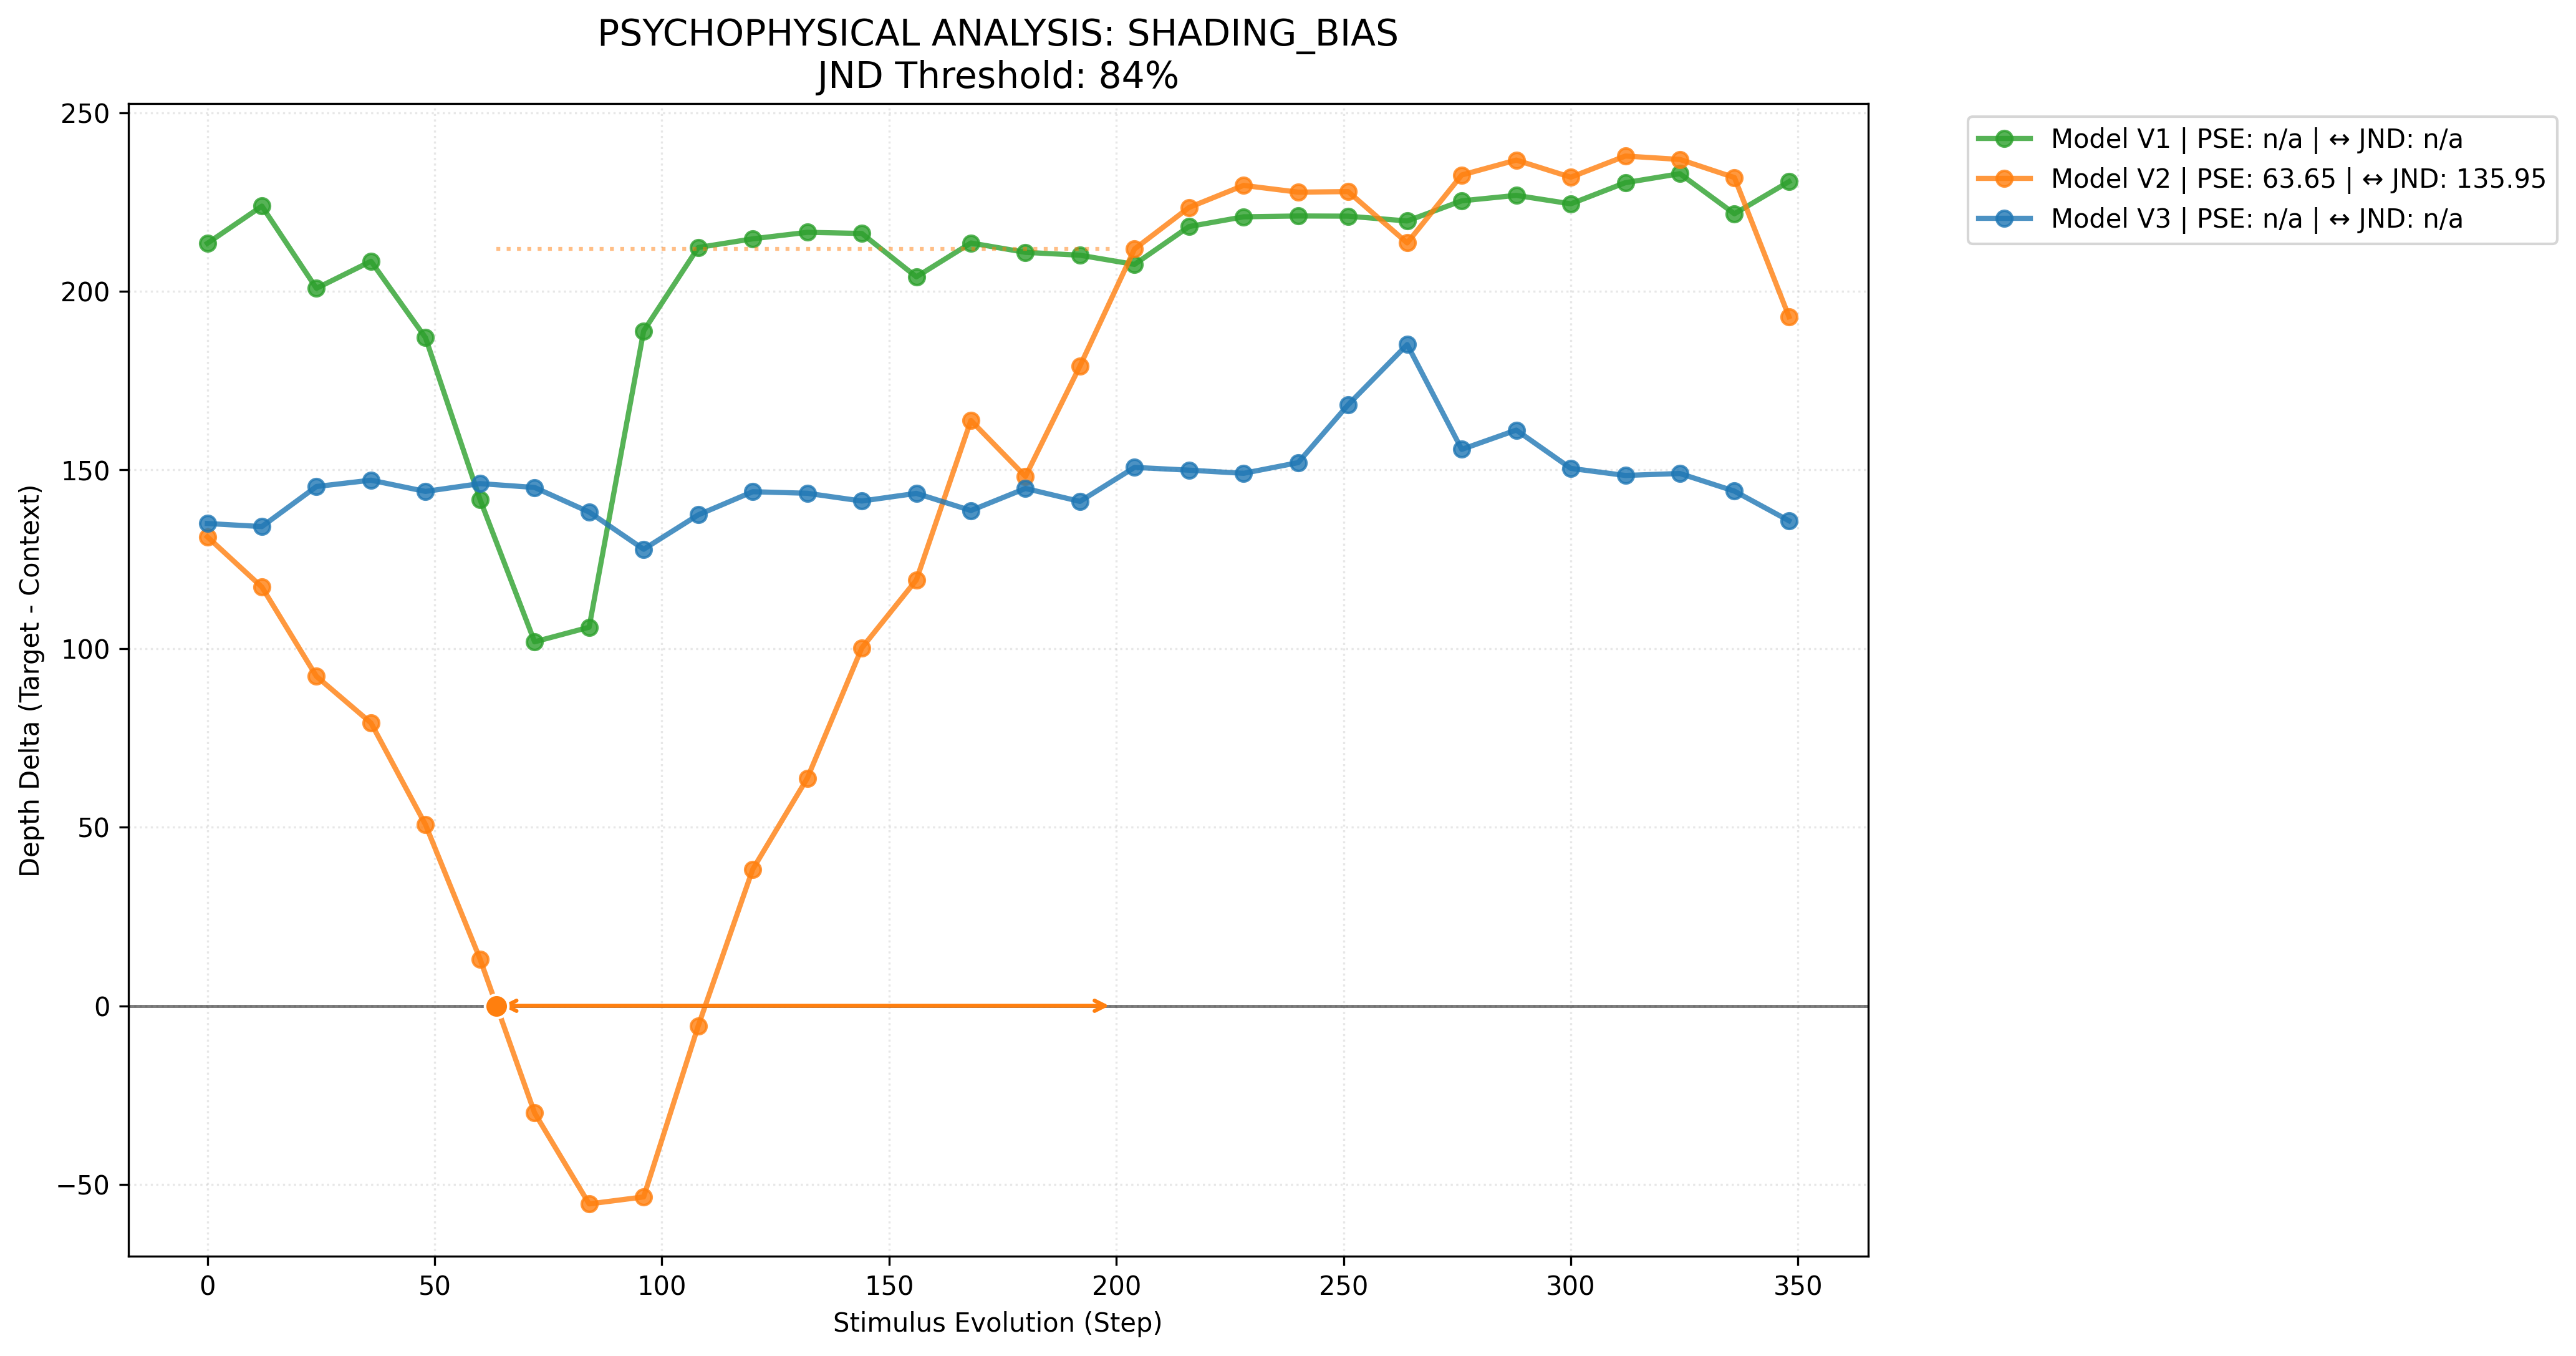
\includegraphics[width=1.02\linewidth]{figures/fig_shading_bias.png}
  \caption{Psychophysical analysis of the Shading photometric bias. The curves depict a highly rigid response in V1 and V3, alongside an unstable perceptual boundary in V2 characterized by extreme localized volatility and a broad numerical spread.}
  \label{fig:shading_bias}
\end{figure}

% 8. Shadow Attachment Bias
\begin{figure}[H]
  \centering
  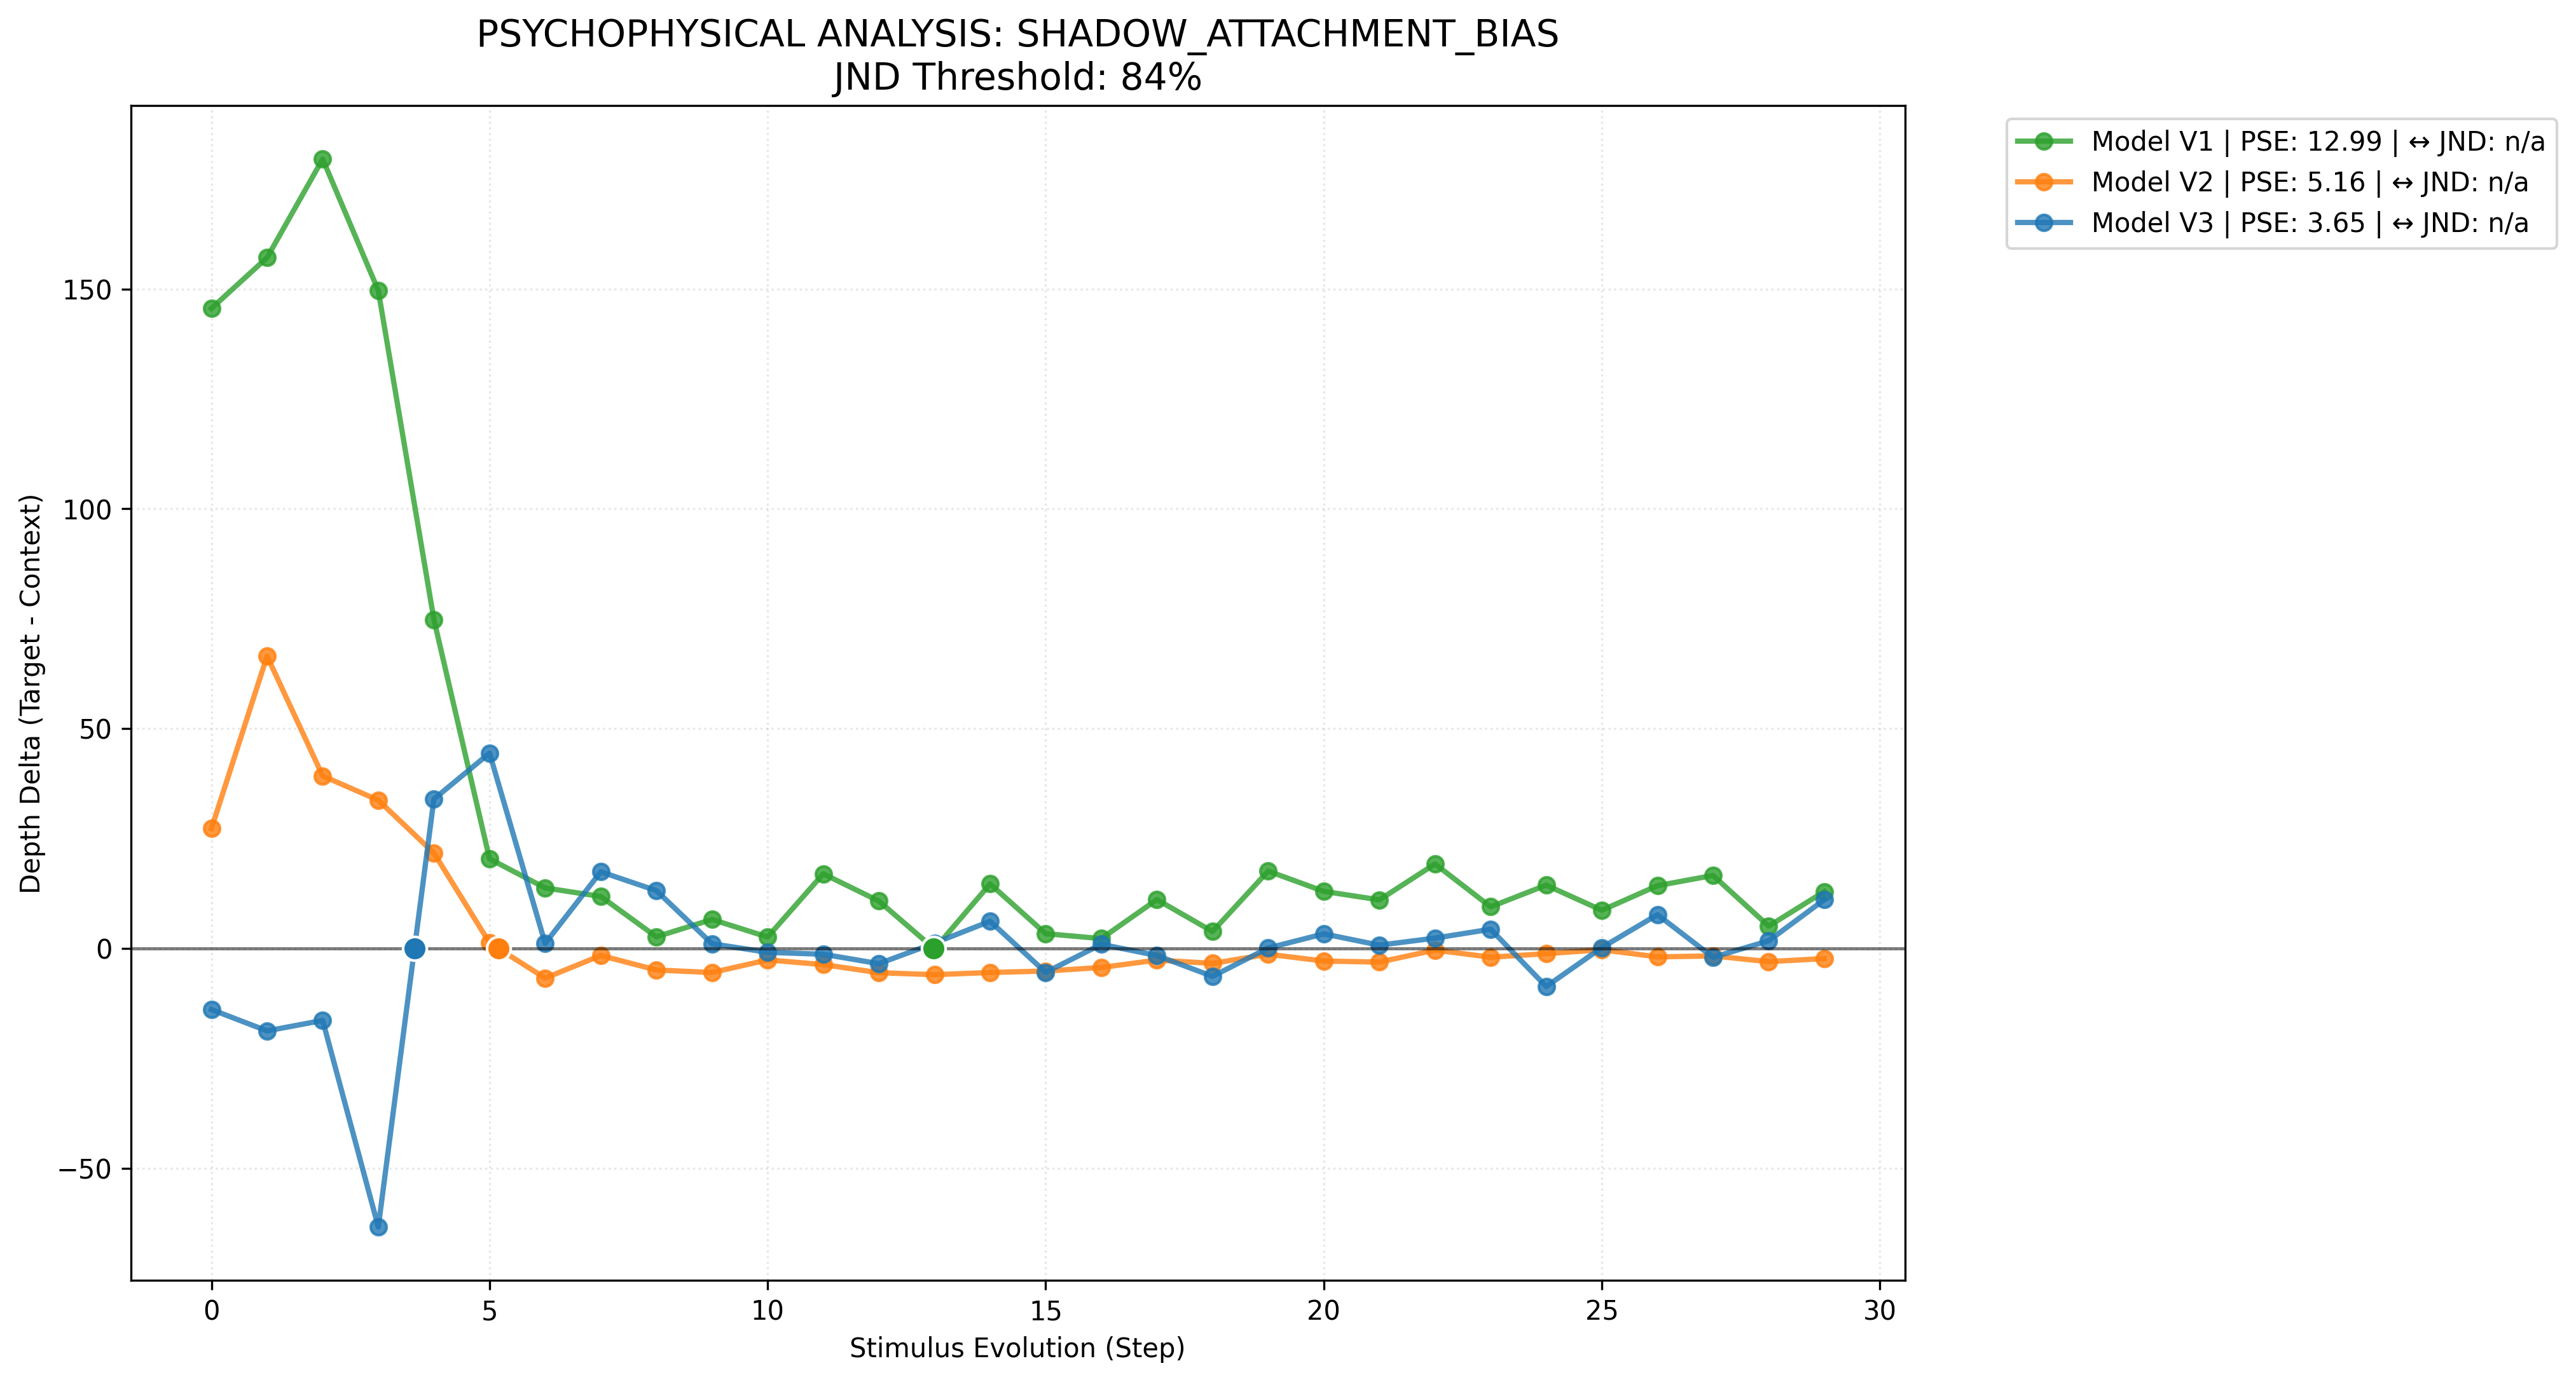
\includegraphics[width=1.02\linewidth]{figures/fig_shadow_attachment_bias.png}
  \caption{Psychophysical analysis of the Shadow Attachment bias. The plot illustrates an immediate, step-like perceptual flip across all architectures, documenting an accelerated commitment to depth ordering driven by modern grounding priors in successive model generations.}
  \label{fig:shadow_attachment_bias}
\end{figure}

% 9. Kanizsa Bias
\begin{figure}[H]
  \centering
  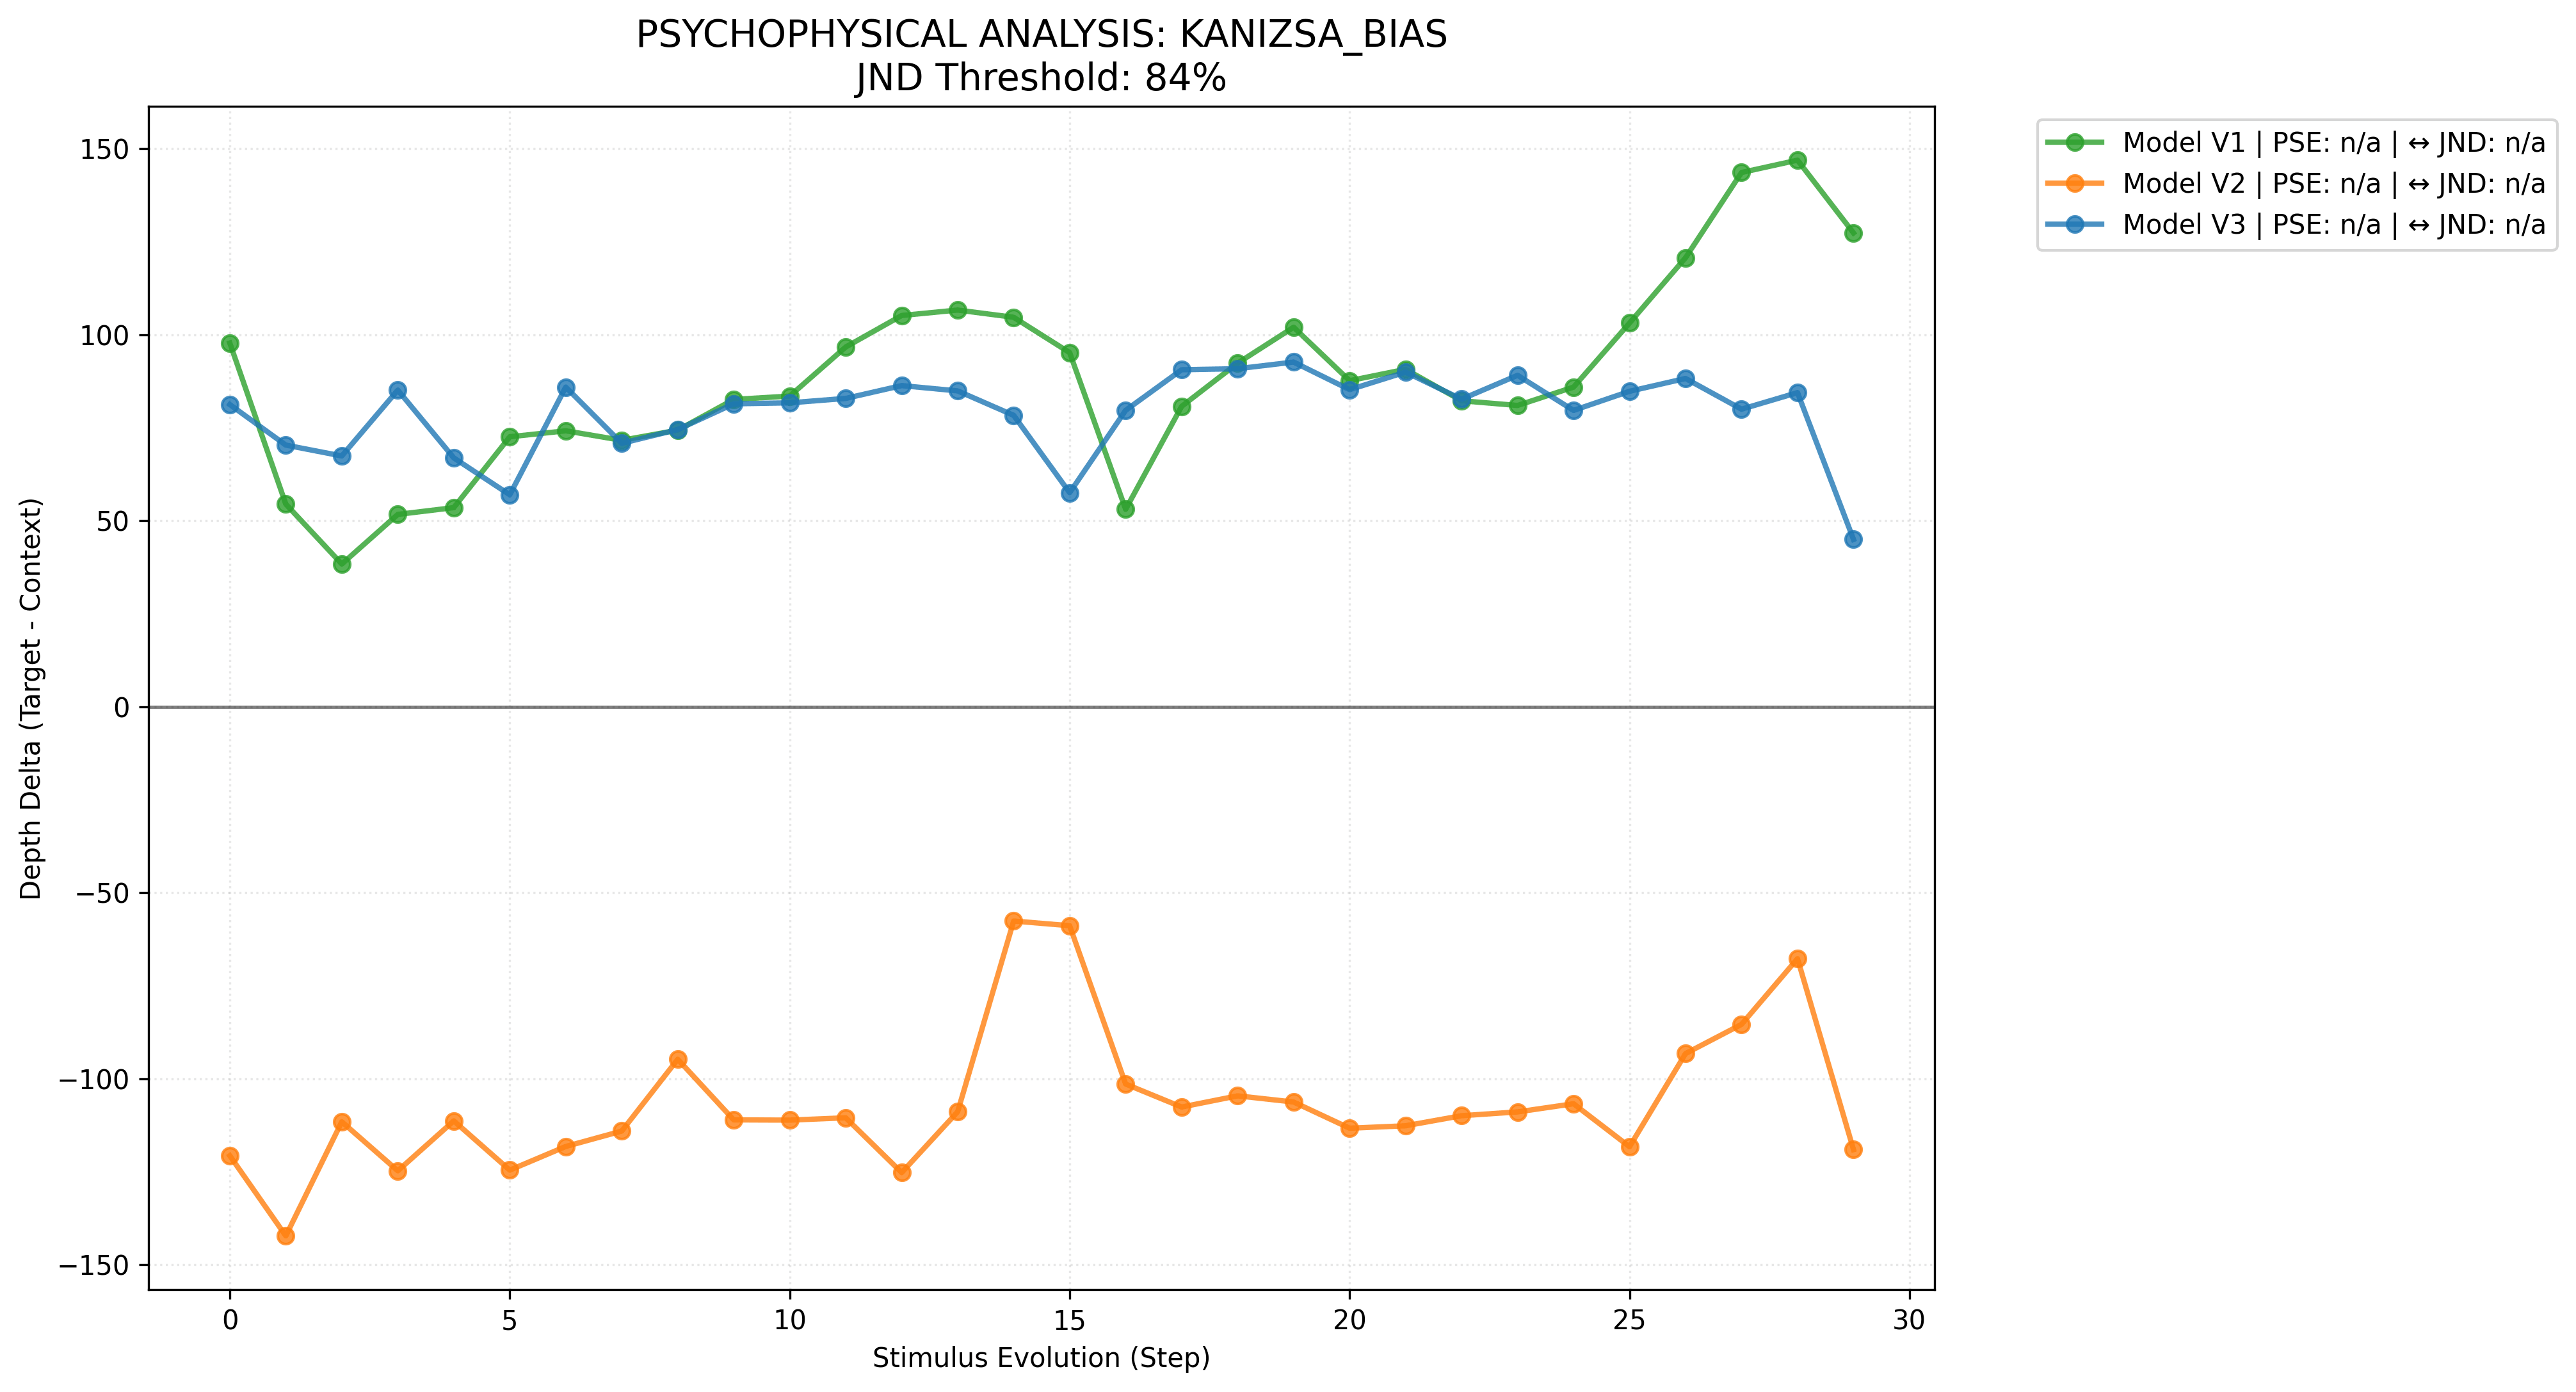
\includegraphics[width=1.02\linewidth]{figures/fig_kanizsa_bias.png}
  \caption{Psychophysical analysis of the Kanizsa illusory-contour bias. The curves track the systematic failure to cross the zero-boundary, highlighting a qualitative perceptual inversion in V2's sign relative to its architectural neighbors (V1 and V3).}
  \label{fig:kanizsa_bias}
\end{figure}

\begin{figure}[H]
  \centering
  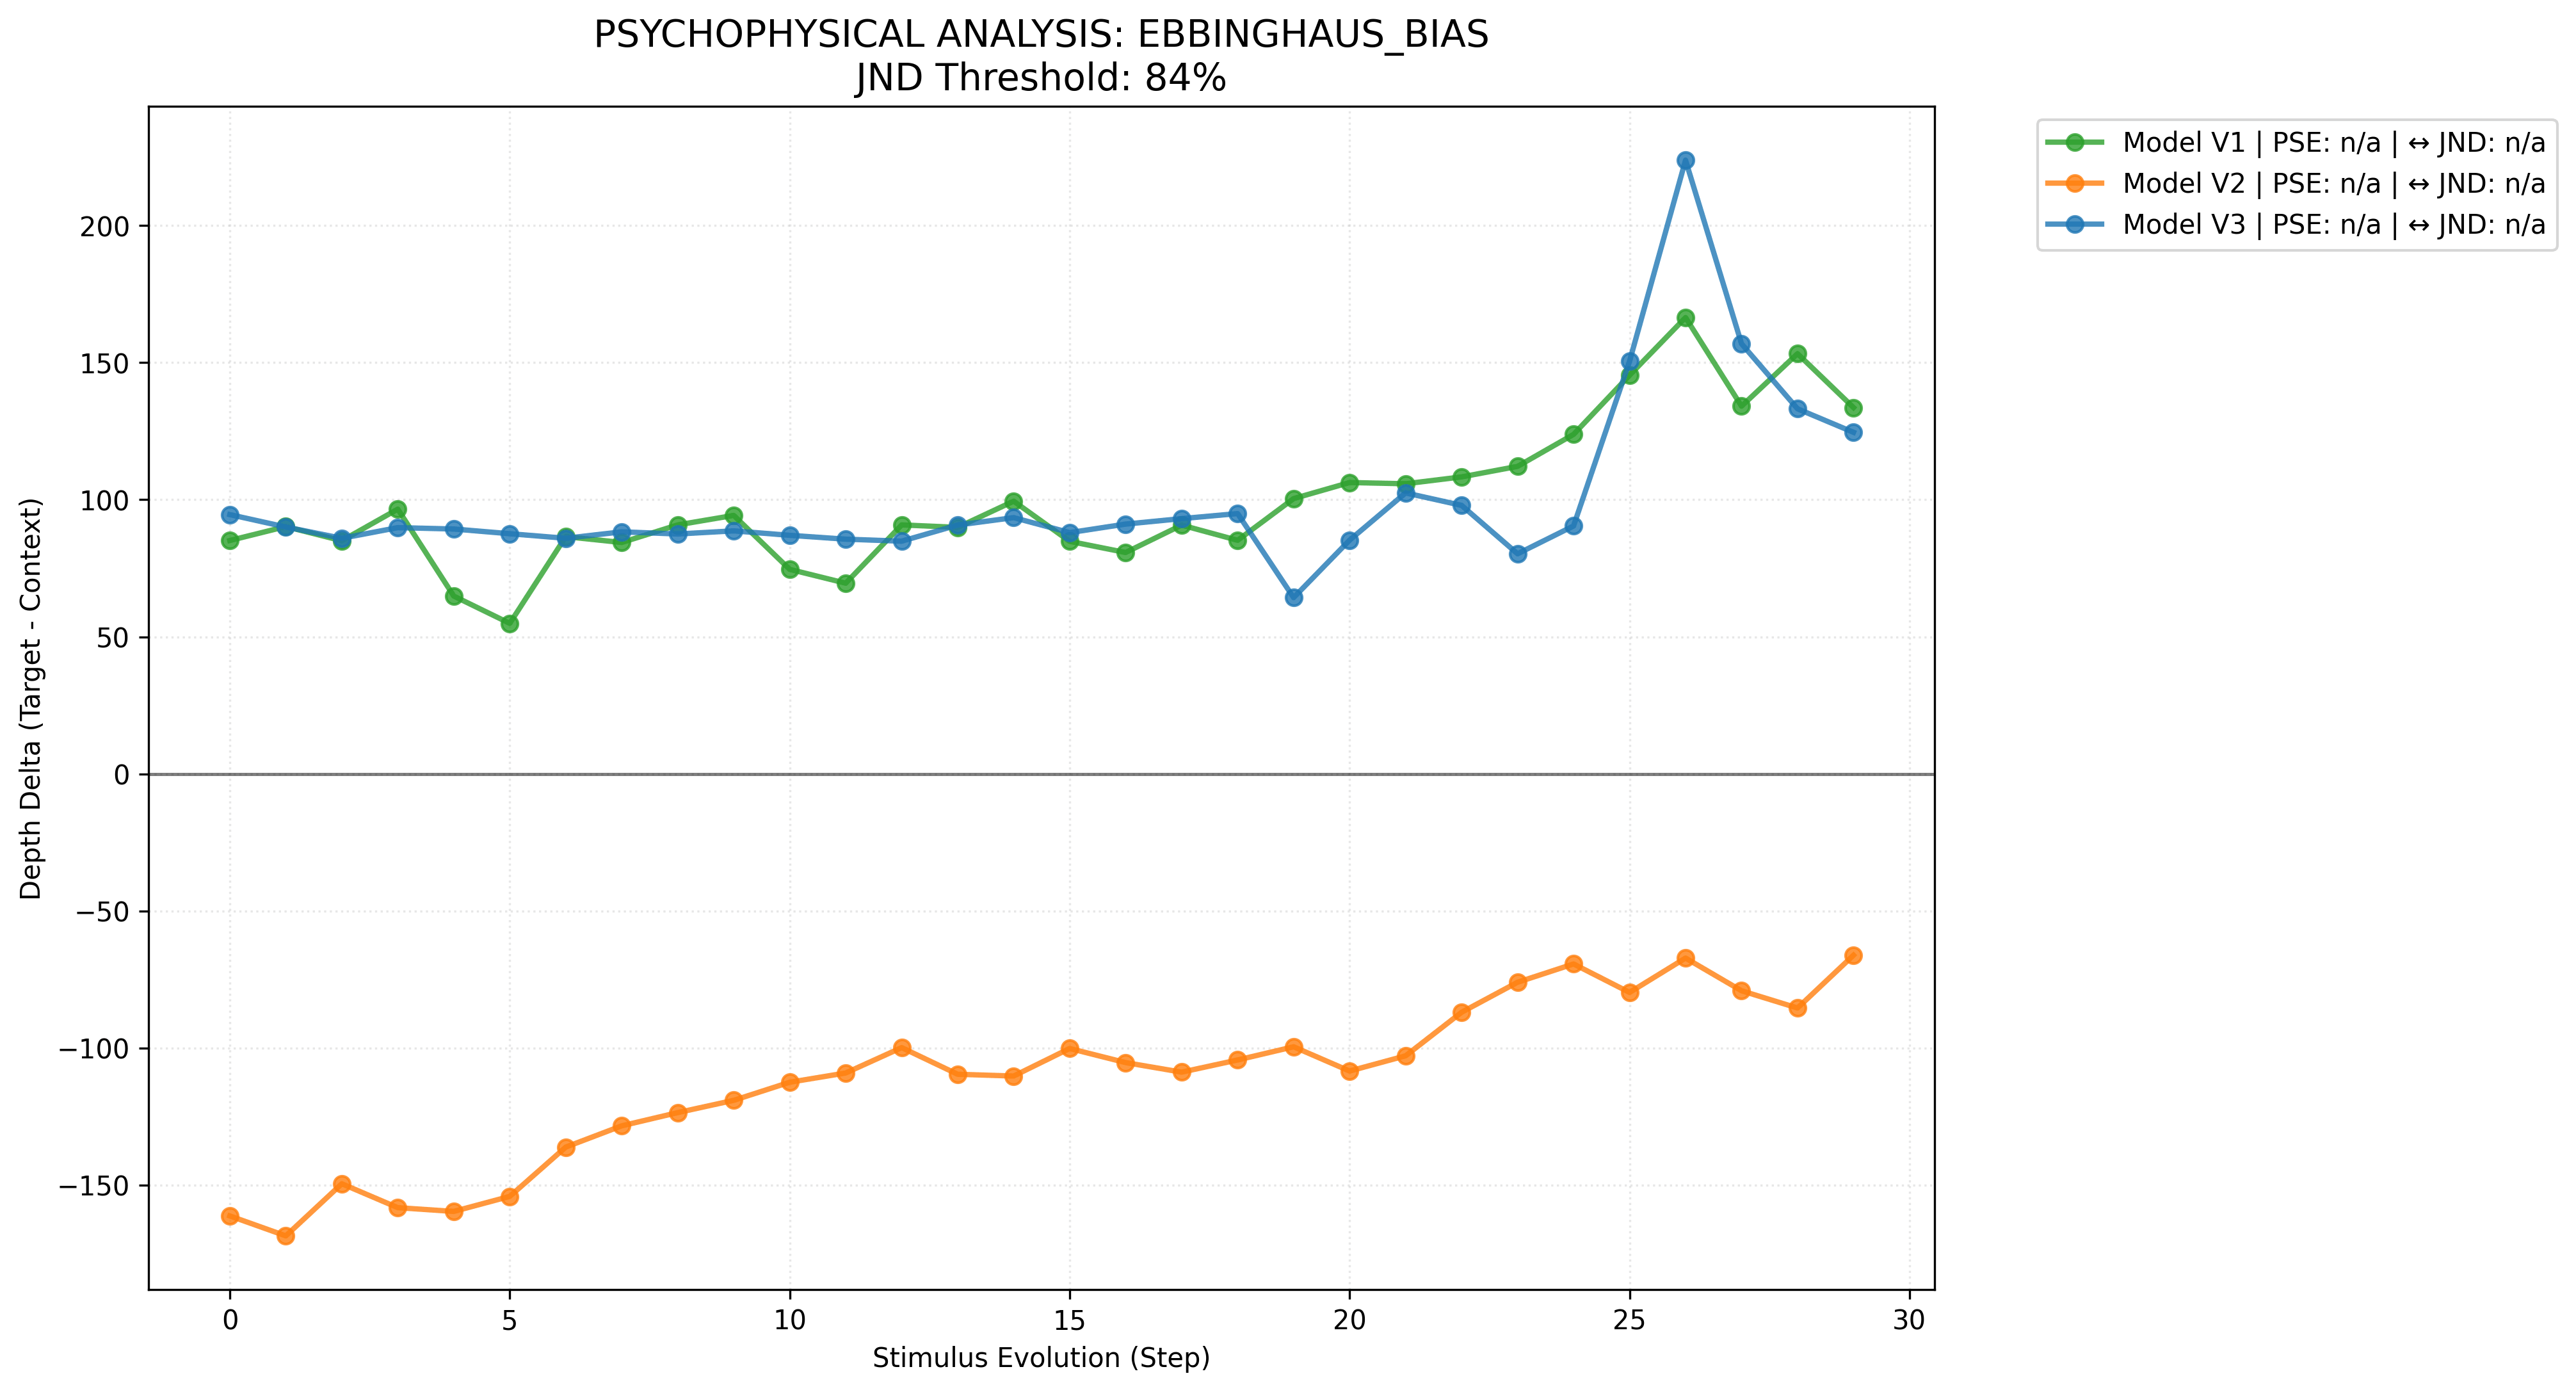
\includegraphics[width=1.02\linewidth]{figures/fig_ebbinghaus_bias.png}
  \caption{Psychophysical analysis of the Ebbinghaus size-contrast bias. The plot tracks the depth delta across the 30-step stimulus evolution, highlighting the absolute stability of the positive bias in V1 and V3 against the inverted negative response of V2.}
  \label{fig:ebbinghaus_bias}
\end{figure}

\begin{figure}[H]
  \centering
  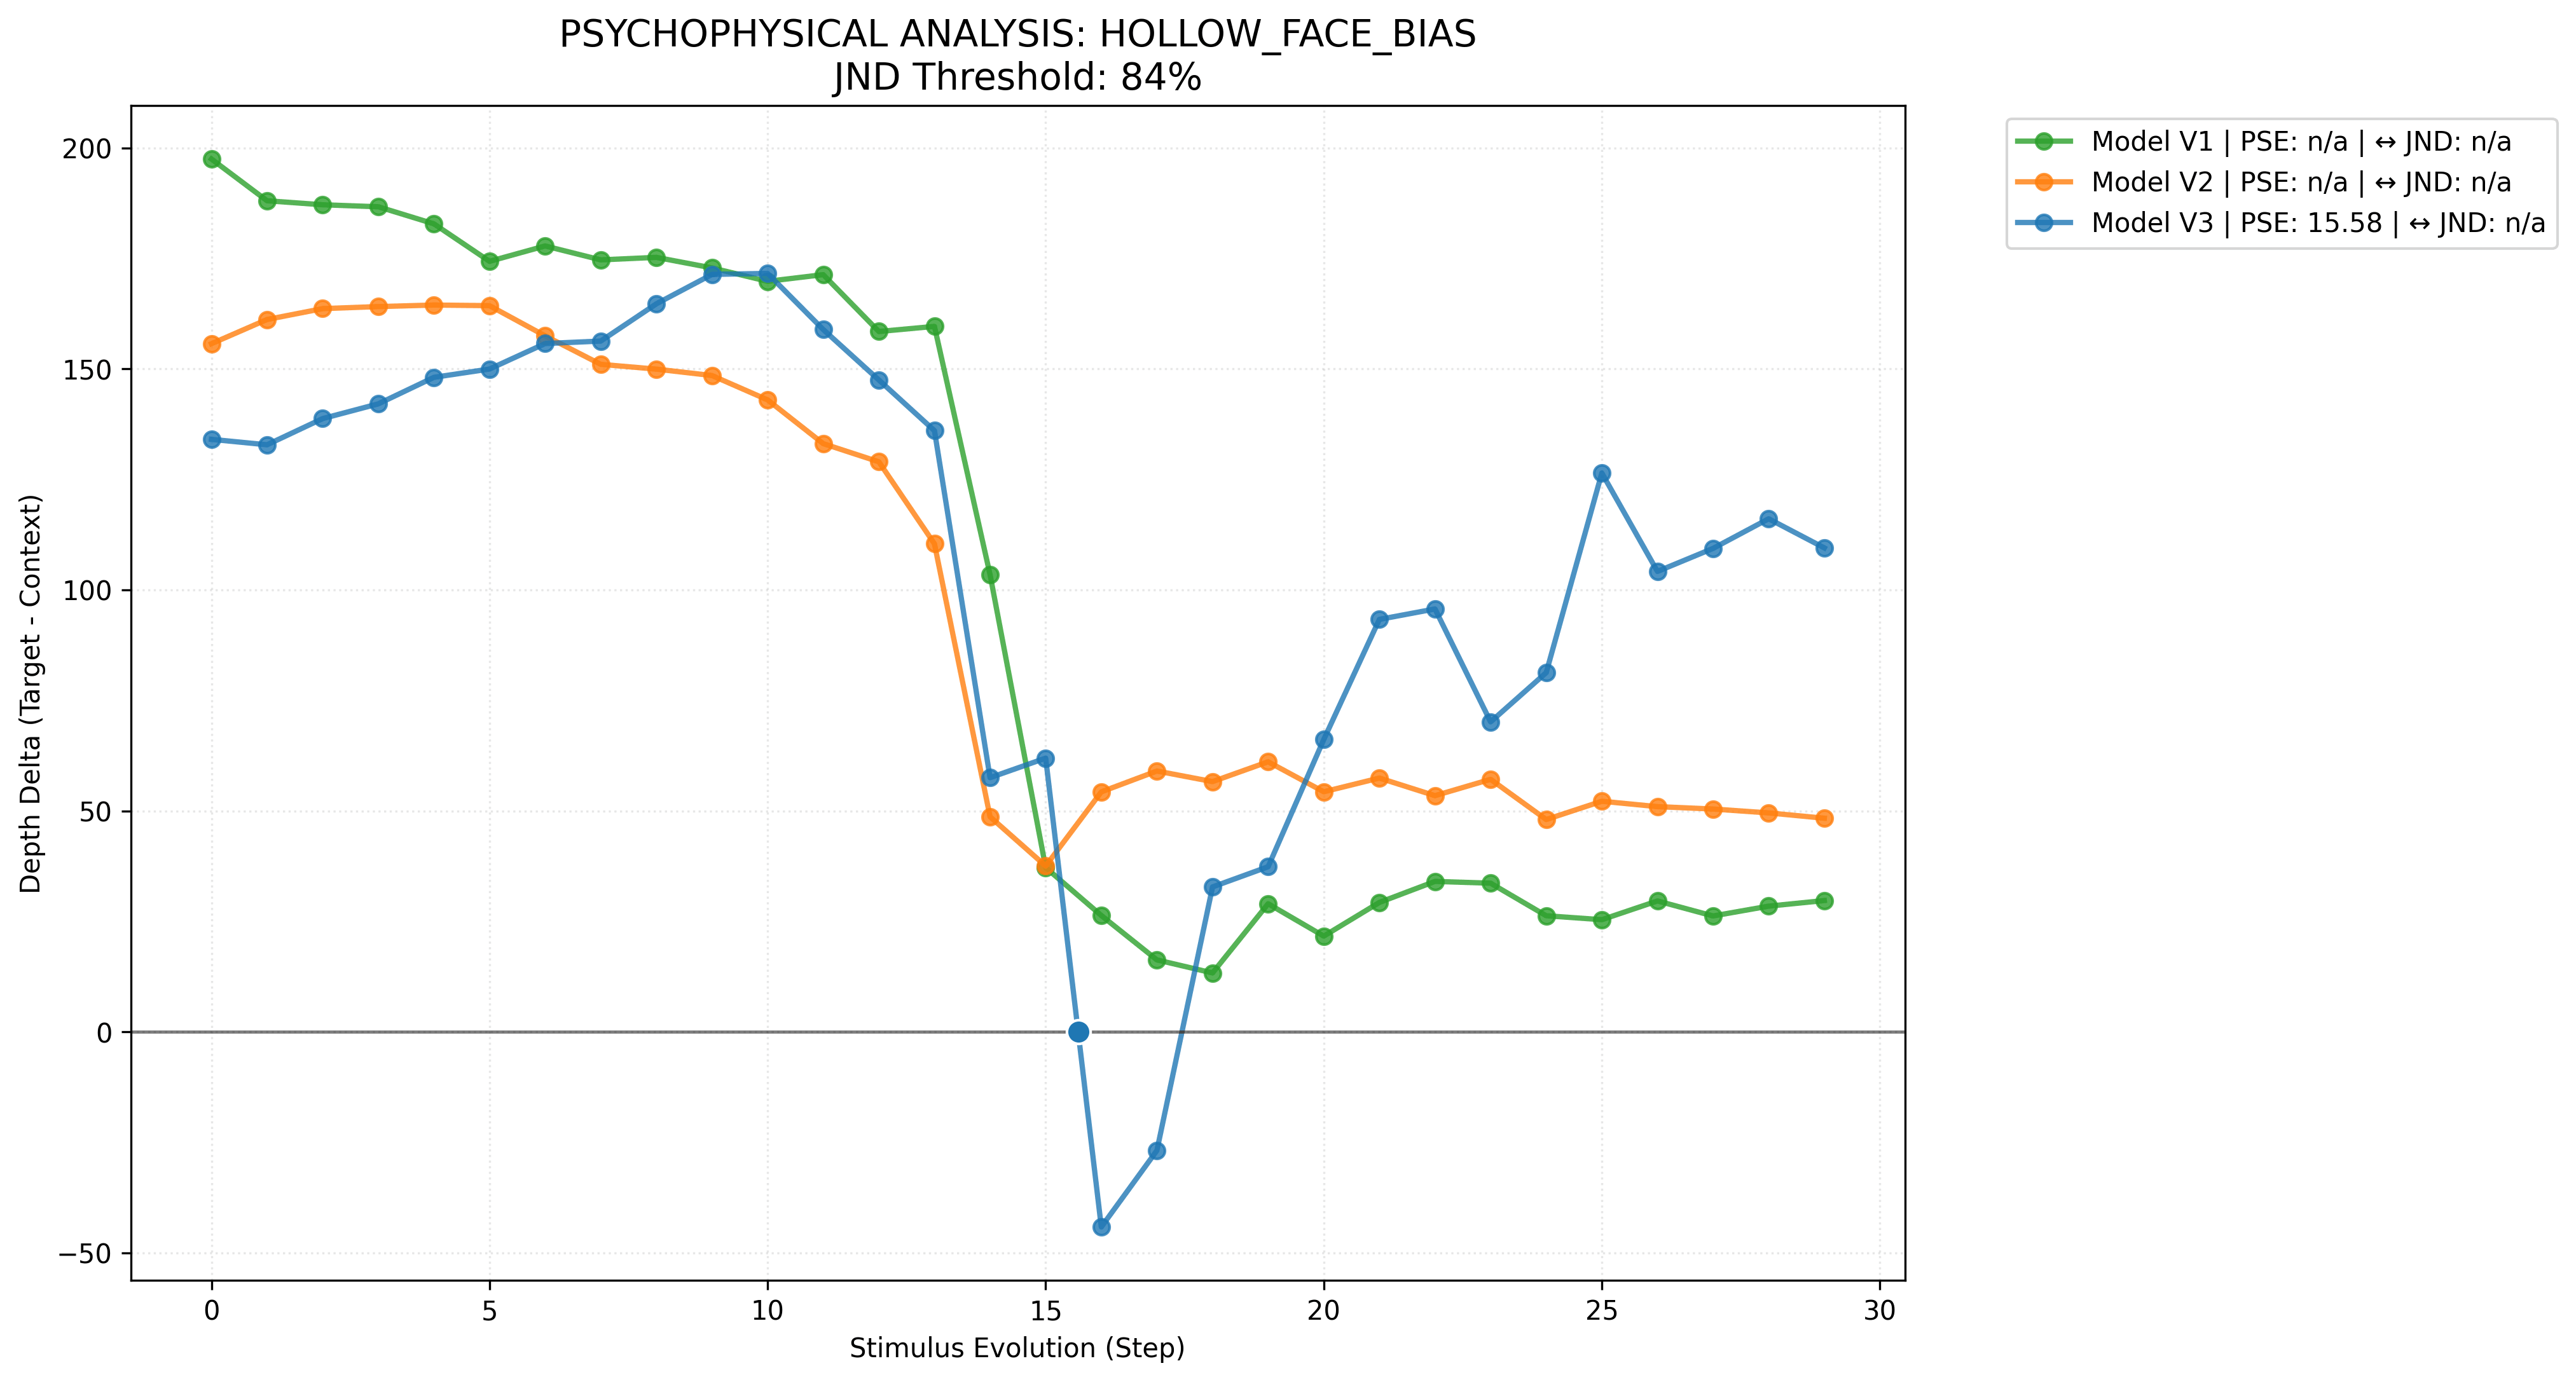
\includegraphics[width=1.02\linewidth]{figures/fig_hollow_face_bias.png}
  \caption{Psychophysical analysis of the Hollow Face bias. The plot isolates the severe vulnerability of V1 and V2 as they remain far from subjective equality, while highlighting V3's capacity to resolve a PSE precisely at the flat-surface baseline where the competing convexity cue is neutralized.}
  \label{fig:hollow_face_bias}
\end{figure}

% 10. Figure-Ground Bias
\begin{figure}[H]
  \centering
  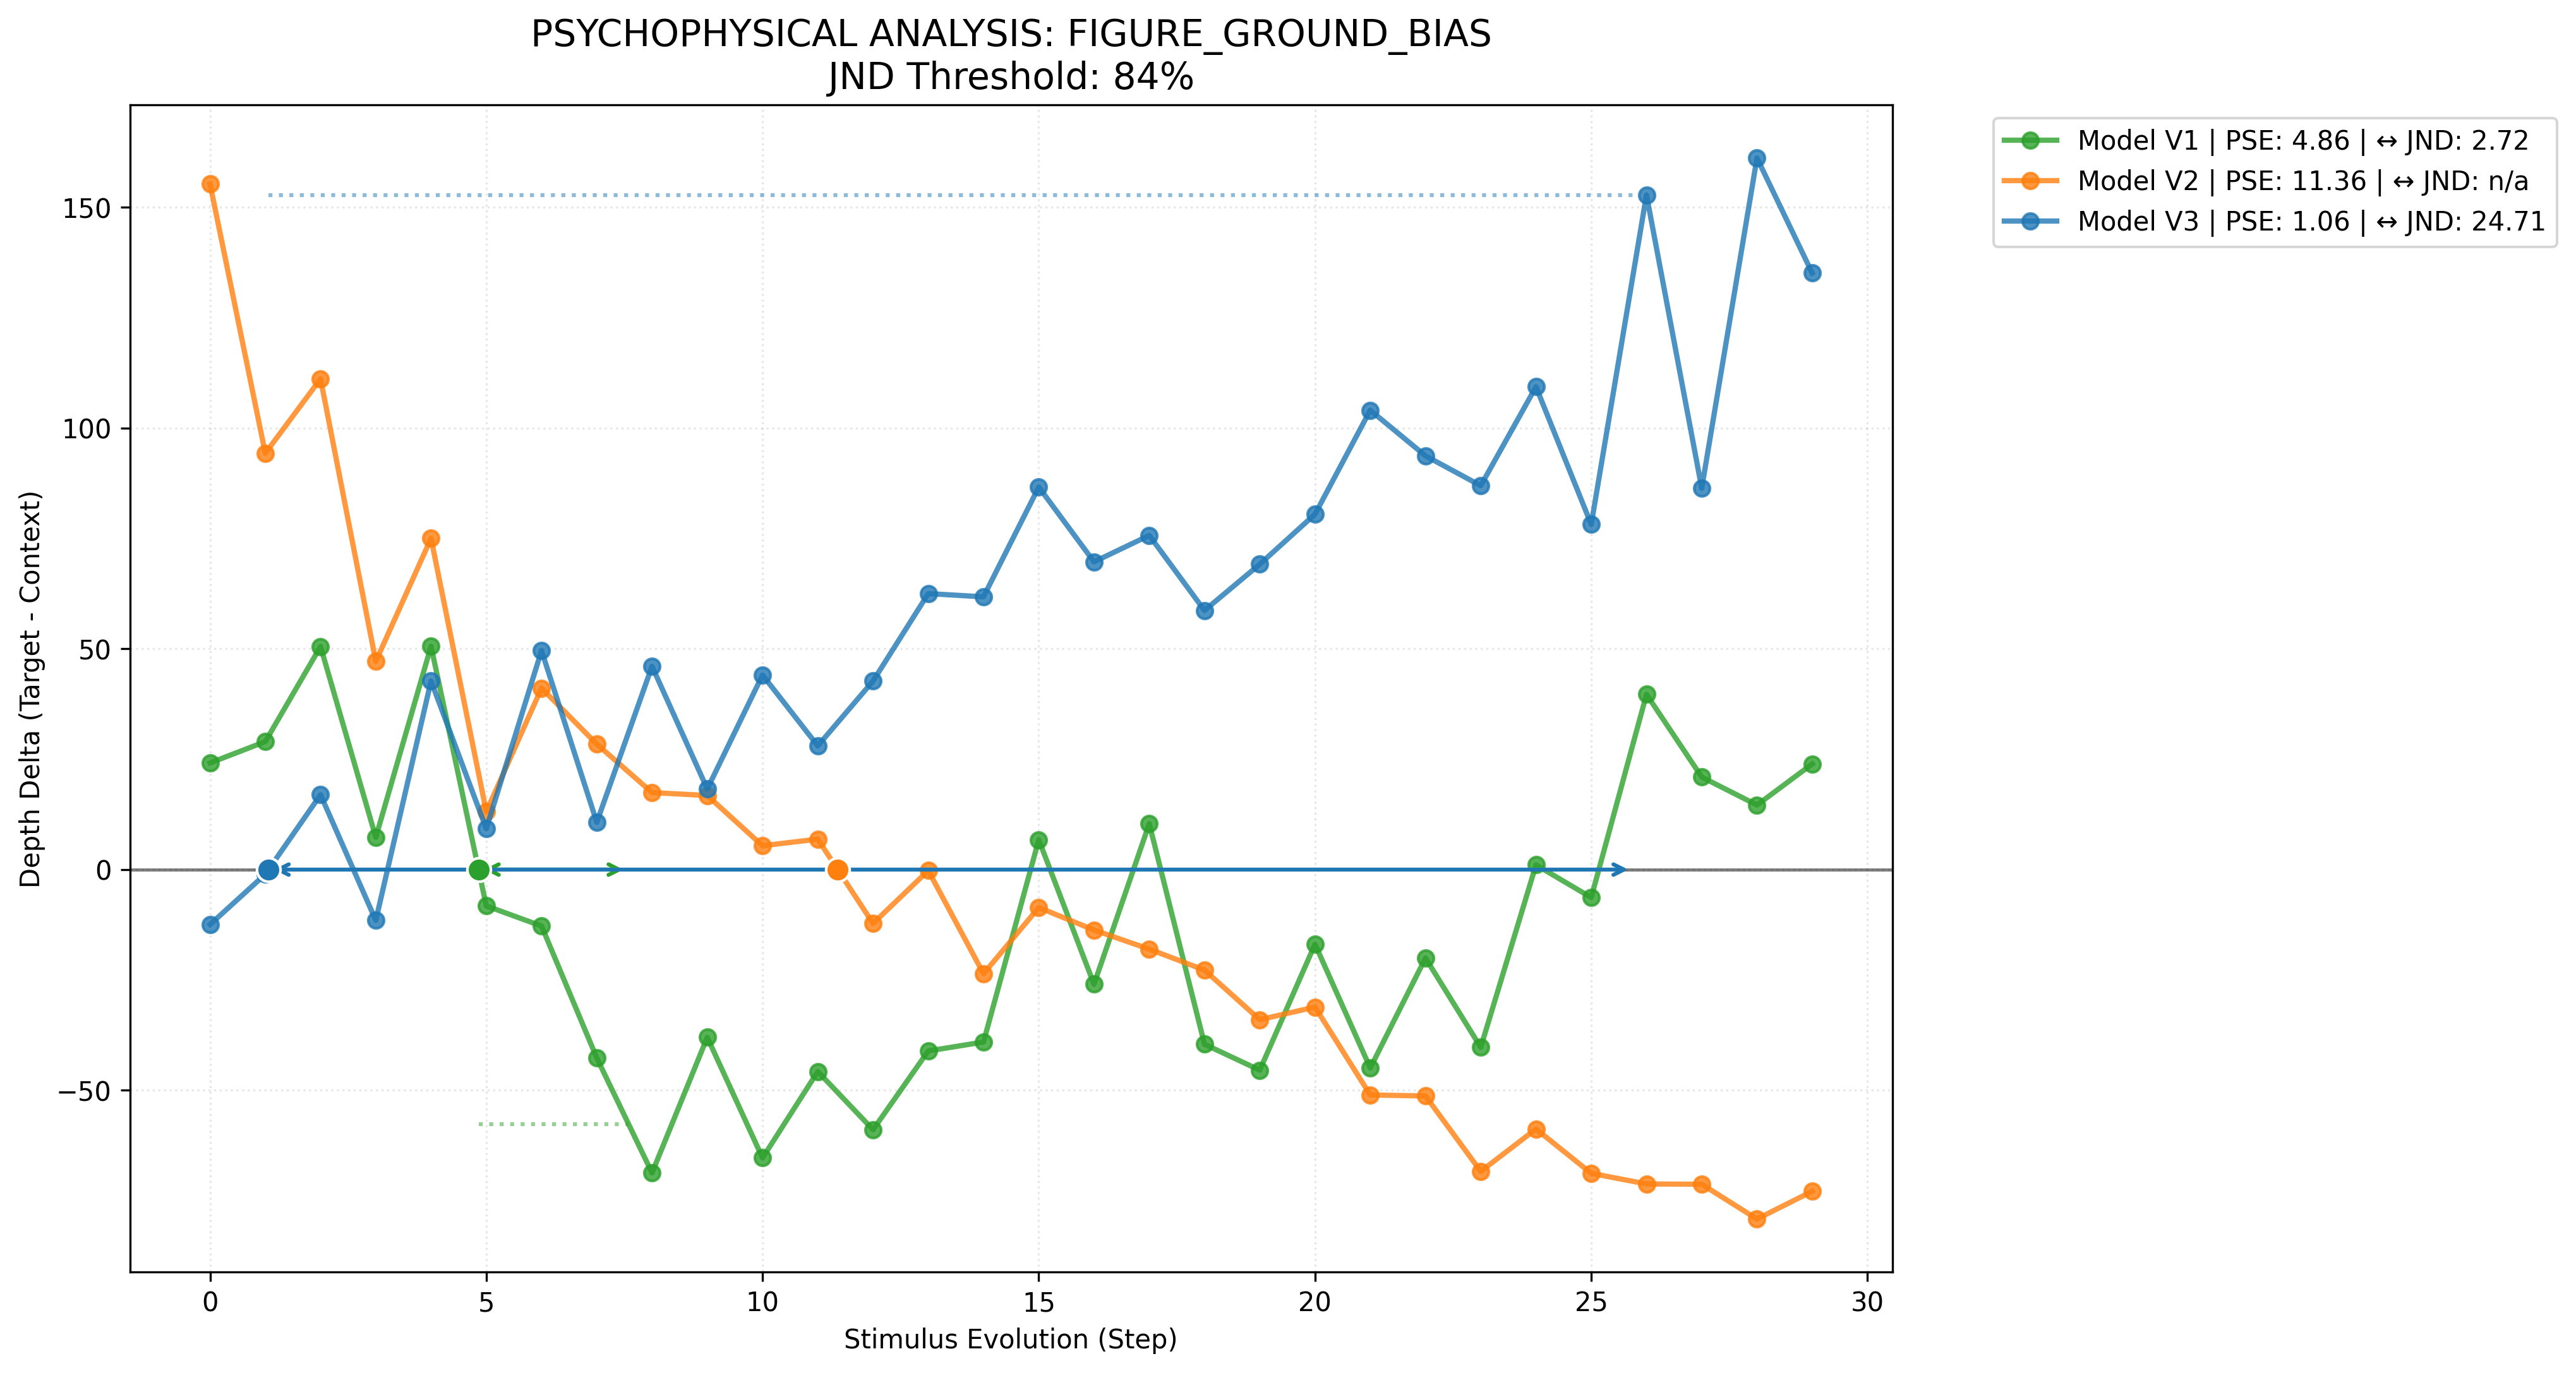
\includegraphics[width=1.02\linewidth]{figures/fig_figure_ground_bias.png}
  \caption{Psychophysical analysis of the ambiguous Figure-Ground bias. The plot captures an exceptionally sharp, low-JND transition for V1 ($JND = 2.72$), contrasted against V2's immediate shift and V3's more gradual, extended resolution curve.}
  \label{fig:figure_ground_bias}
\end{figure}

% 11. Occlusion Bias
\begin{figure}[H]
  \centering
  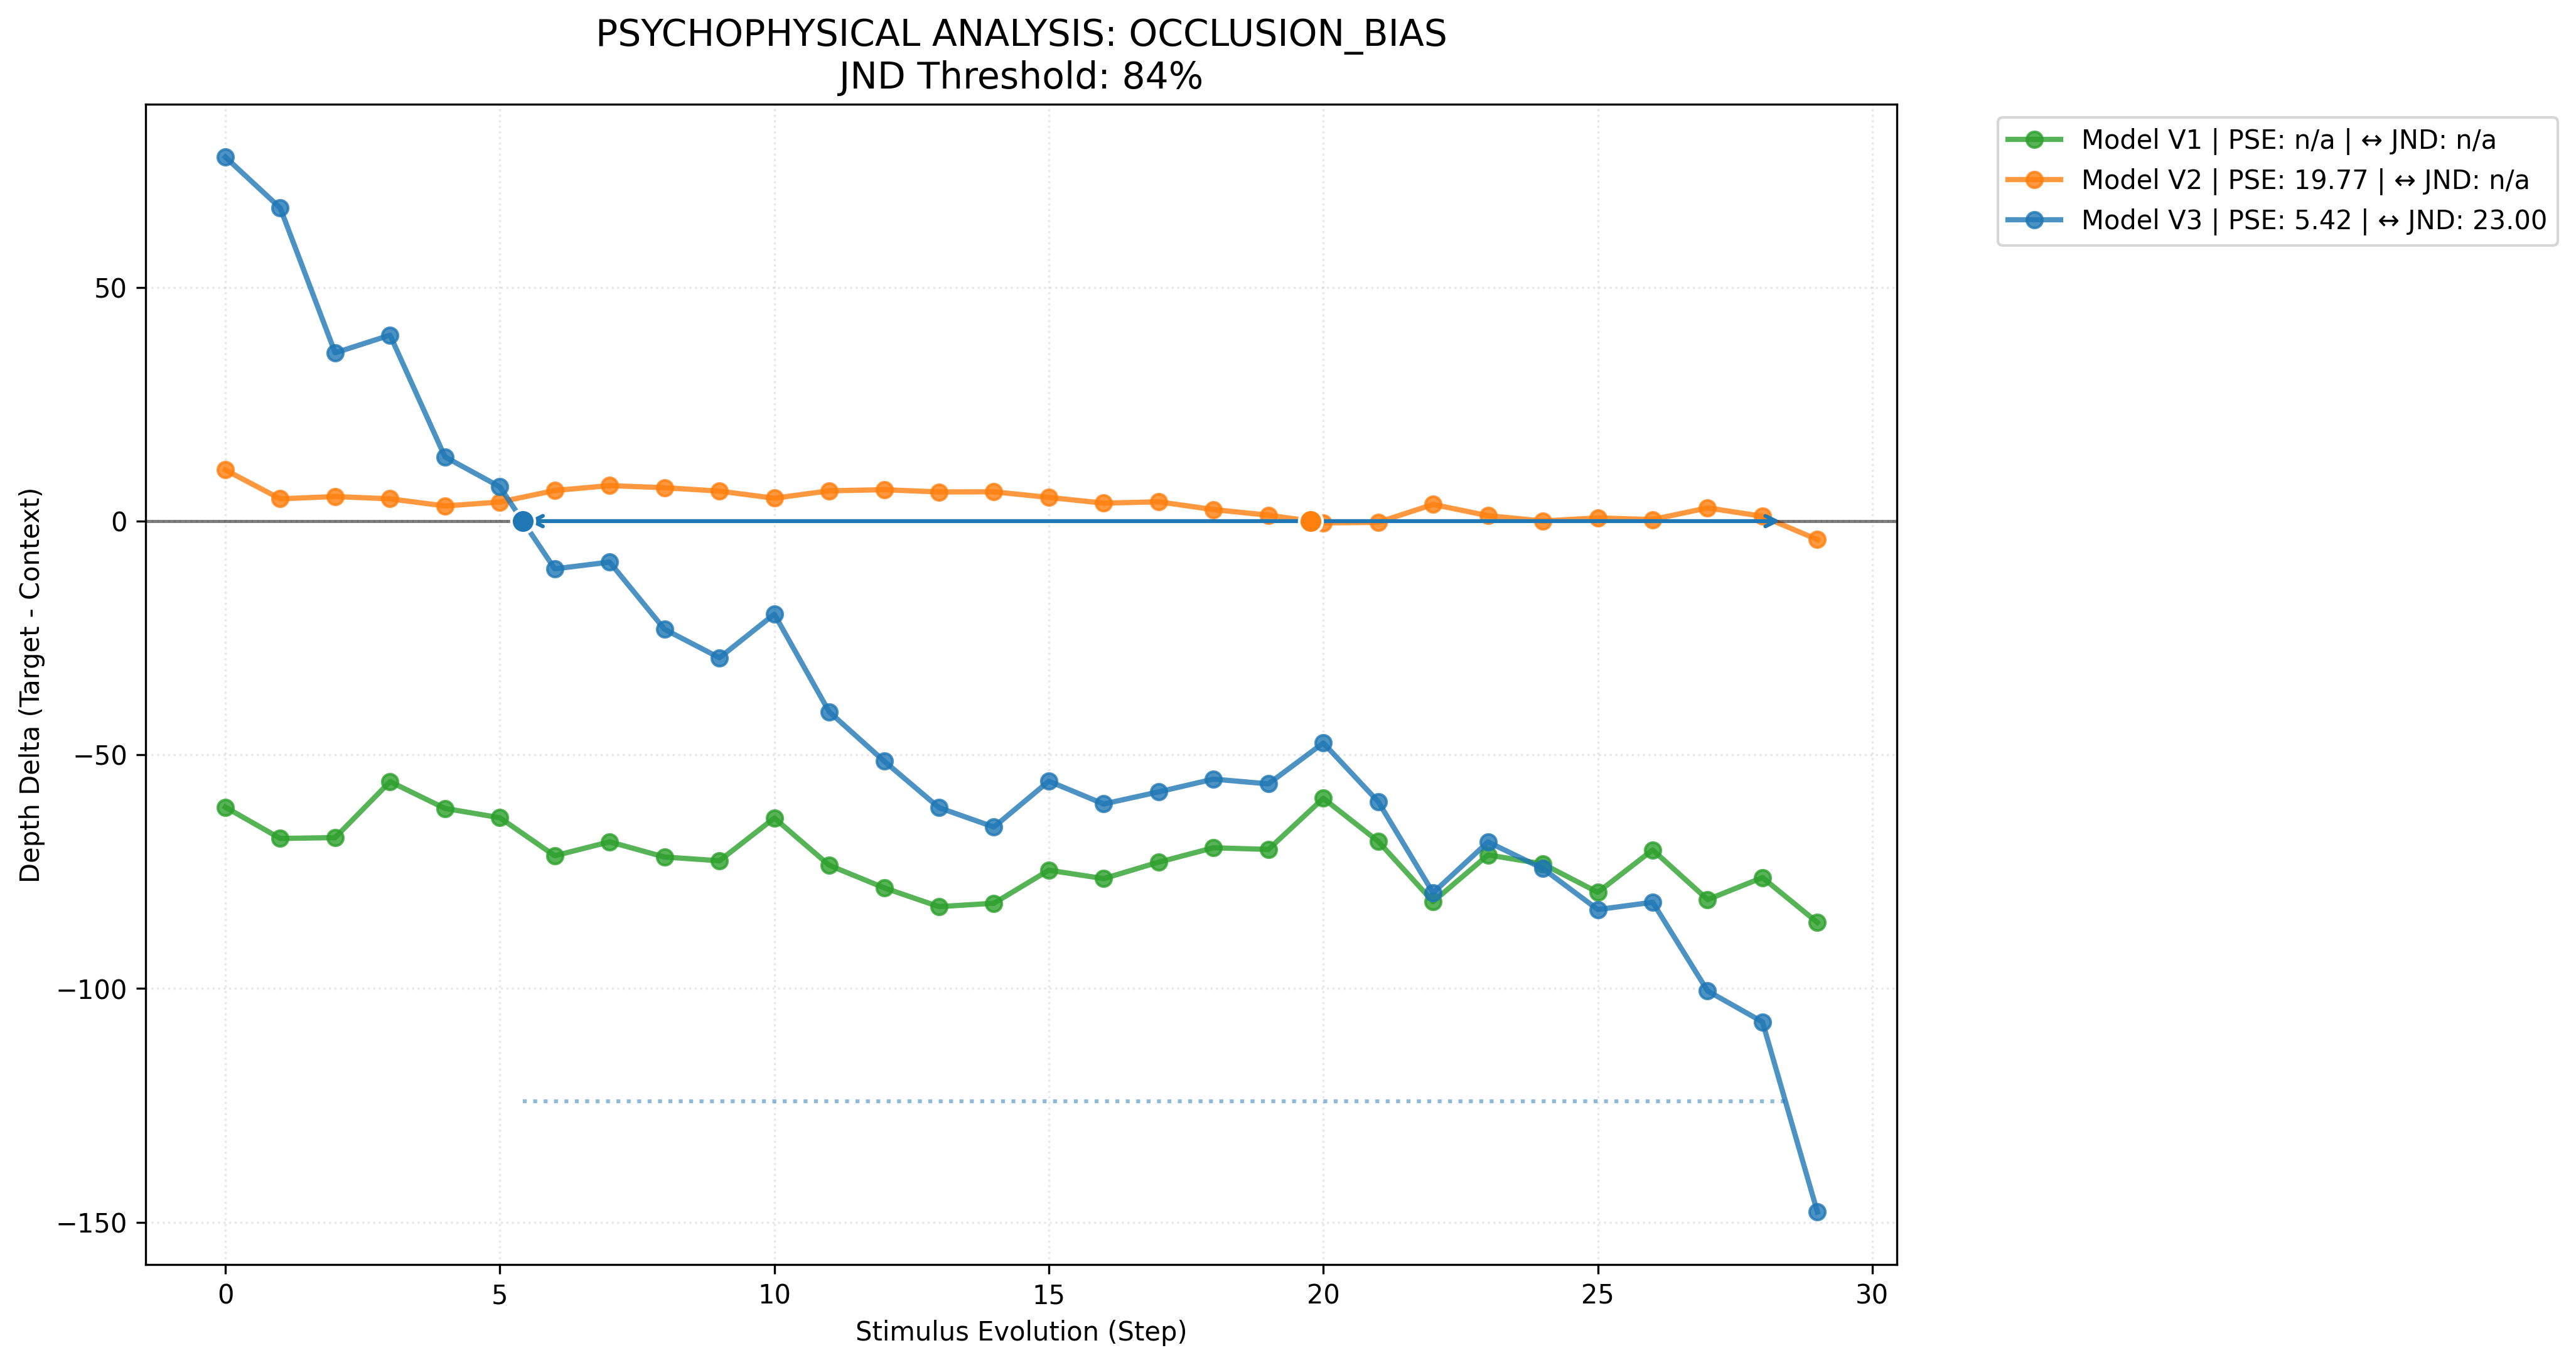
\includegraphics[width=1.02\linewidth]{figures/fig_occlusion_bias.png}
  \caption{Psychophysical analysis of the Occlusion bias. The trajectories illustrate V1's failure to resolve equality, V2's late abrupt shift, and V3's early perceptual flip ($PSE = 5.4$) triggered as the overlapping region's transparency crosses the midpoint boundary.}
  \label{fig:occlusion_bias}
\end{figure}

\subsubsection*{D. MiDaS Quantitative Psychophysical Response Profiles}
\label{app:midas_psychophysics_curves}

\begin{figure}[H]
  \centering
     \begin{subfigure}[b]{0.49\linewidth}
        \centering
        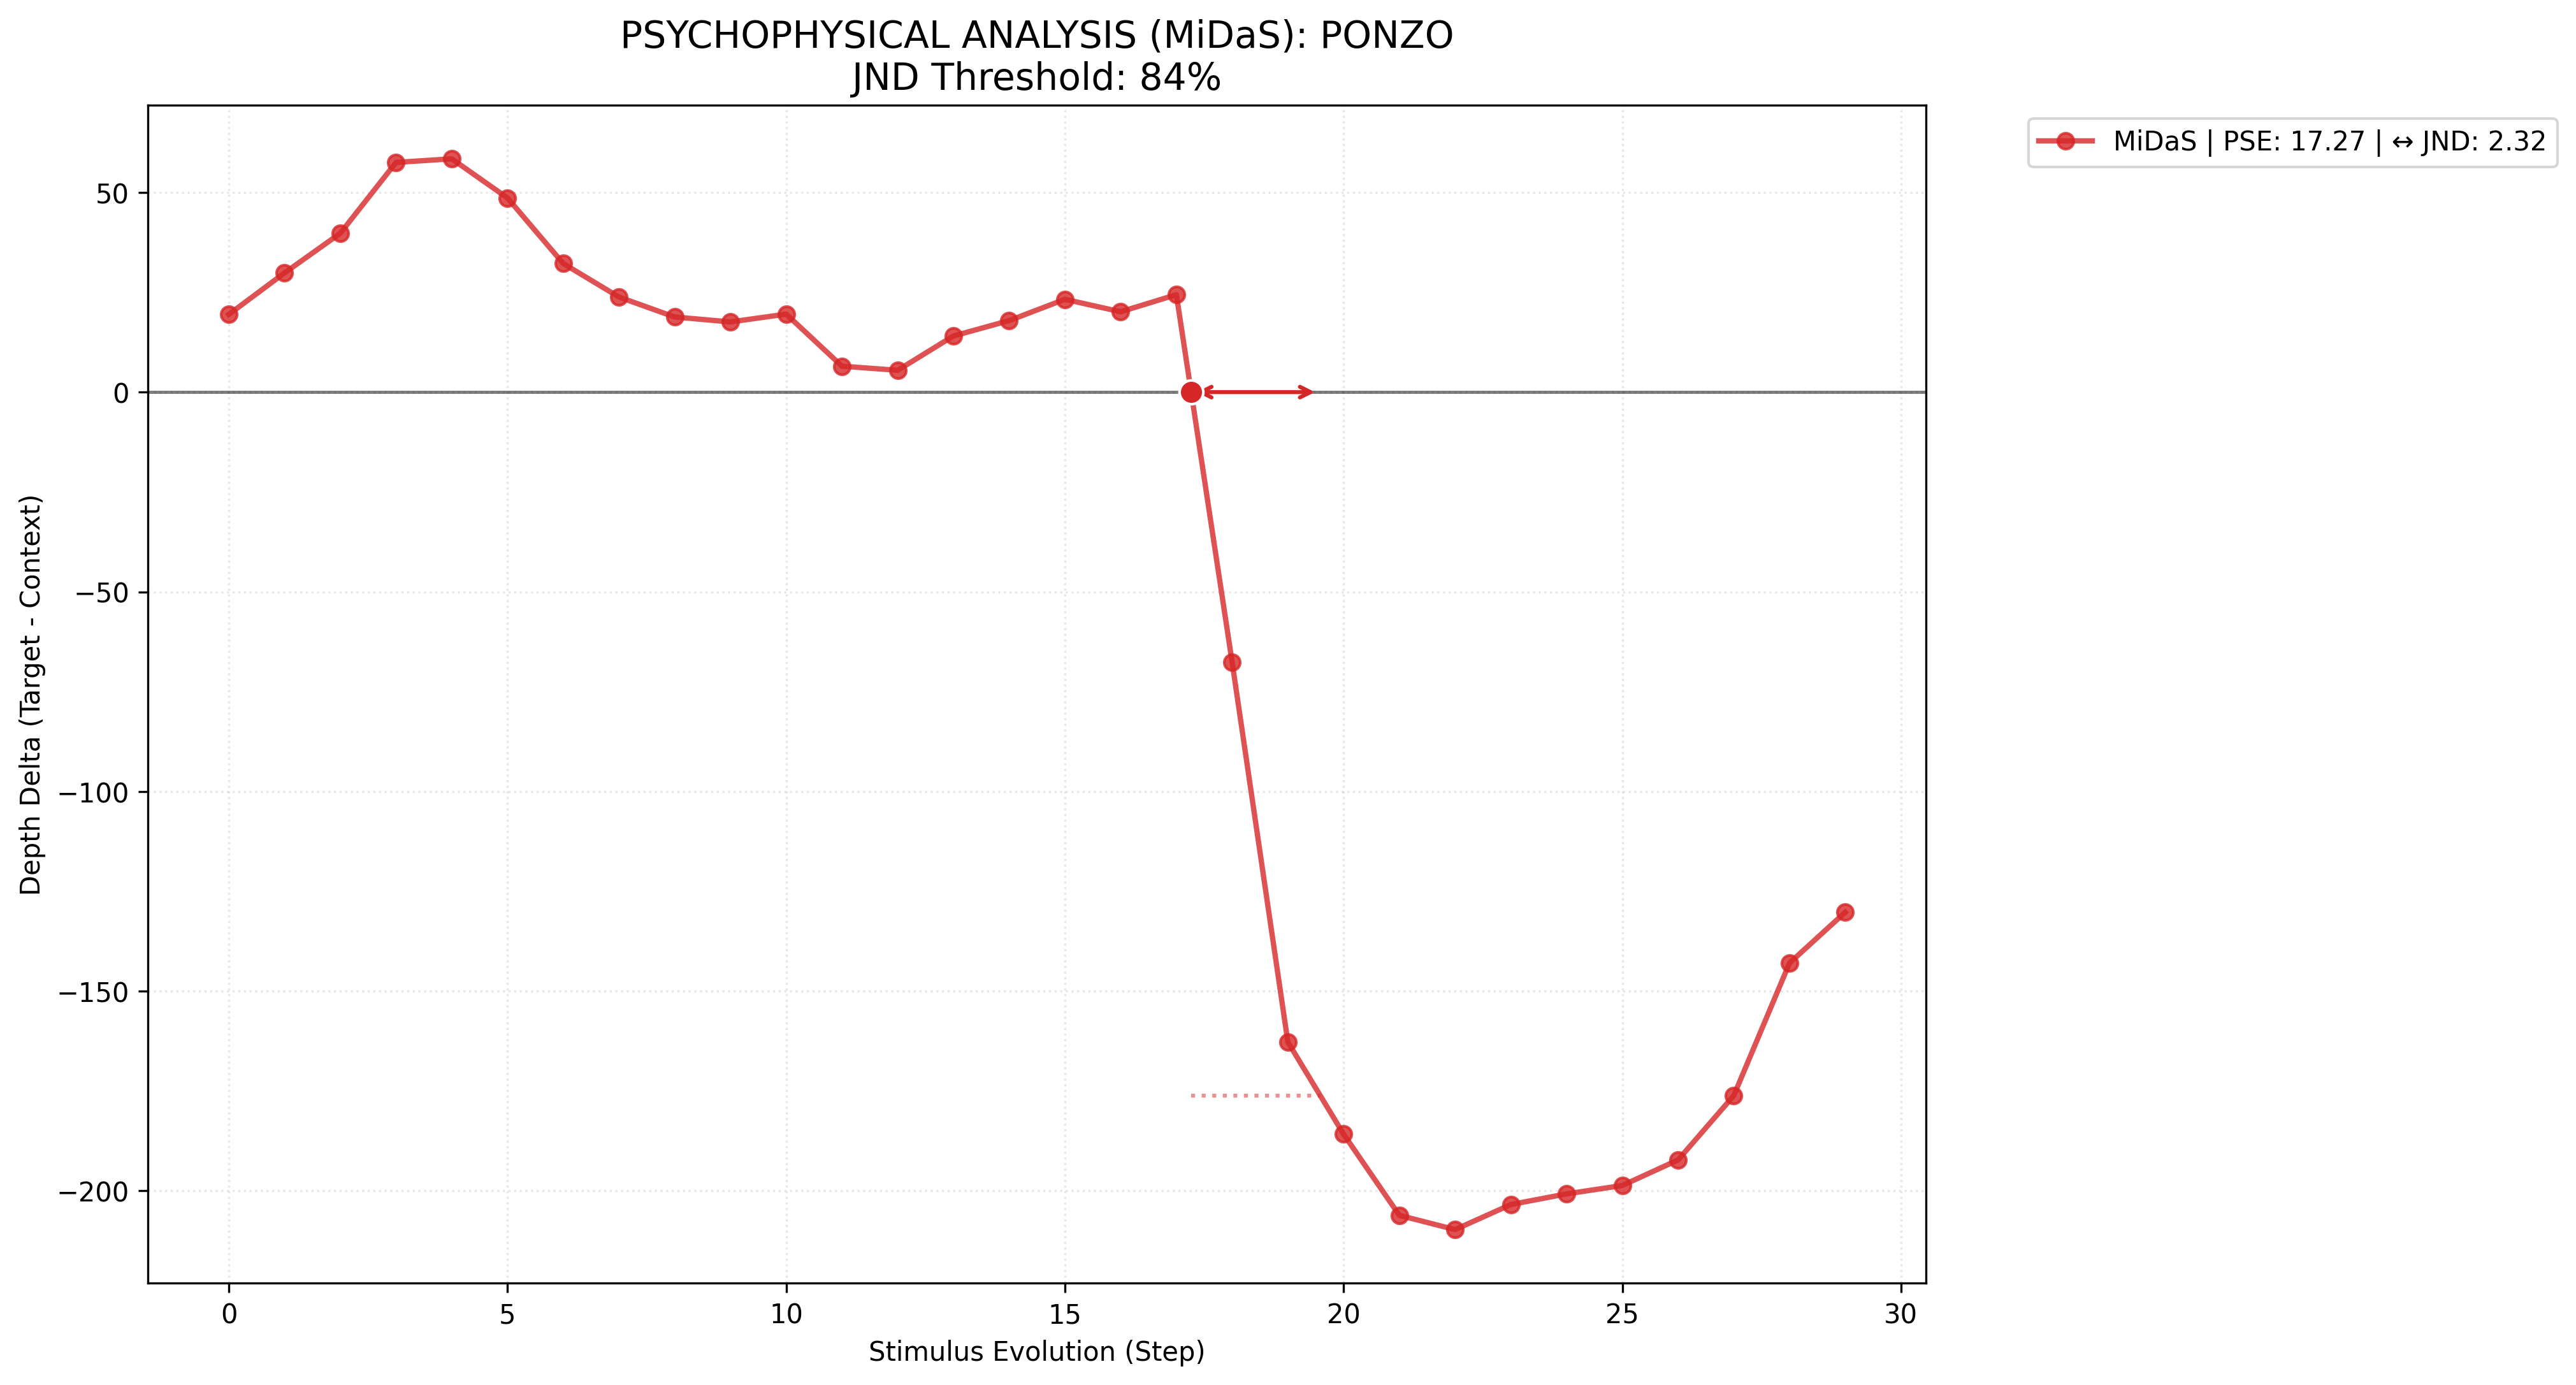
\includegraphics[width=\linewidth]{figures/fig_midas_psy_ponzo.png}
        \caption{Ponzo Illusion (Categorical Step)}
        \label{fig:fig_midas_psy_ponzo}
     \end{subfigure}
     \hfill
     \begin{subfigure}[b]{0.49\linewidth}
        \centering
        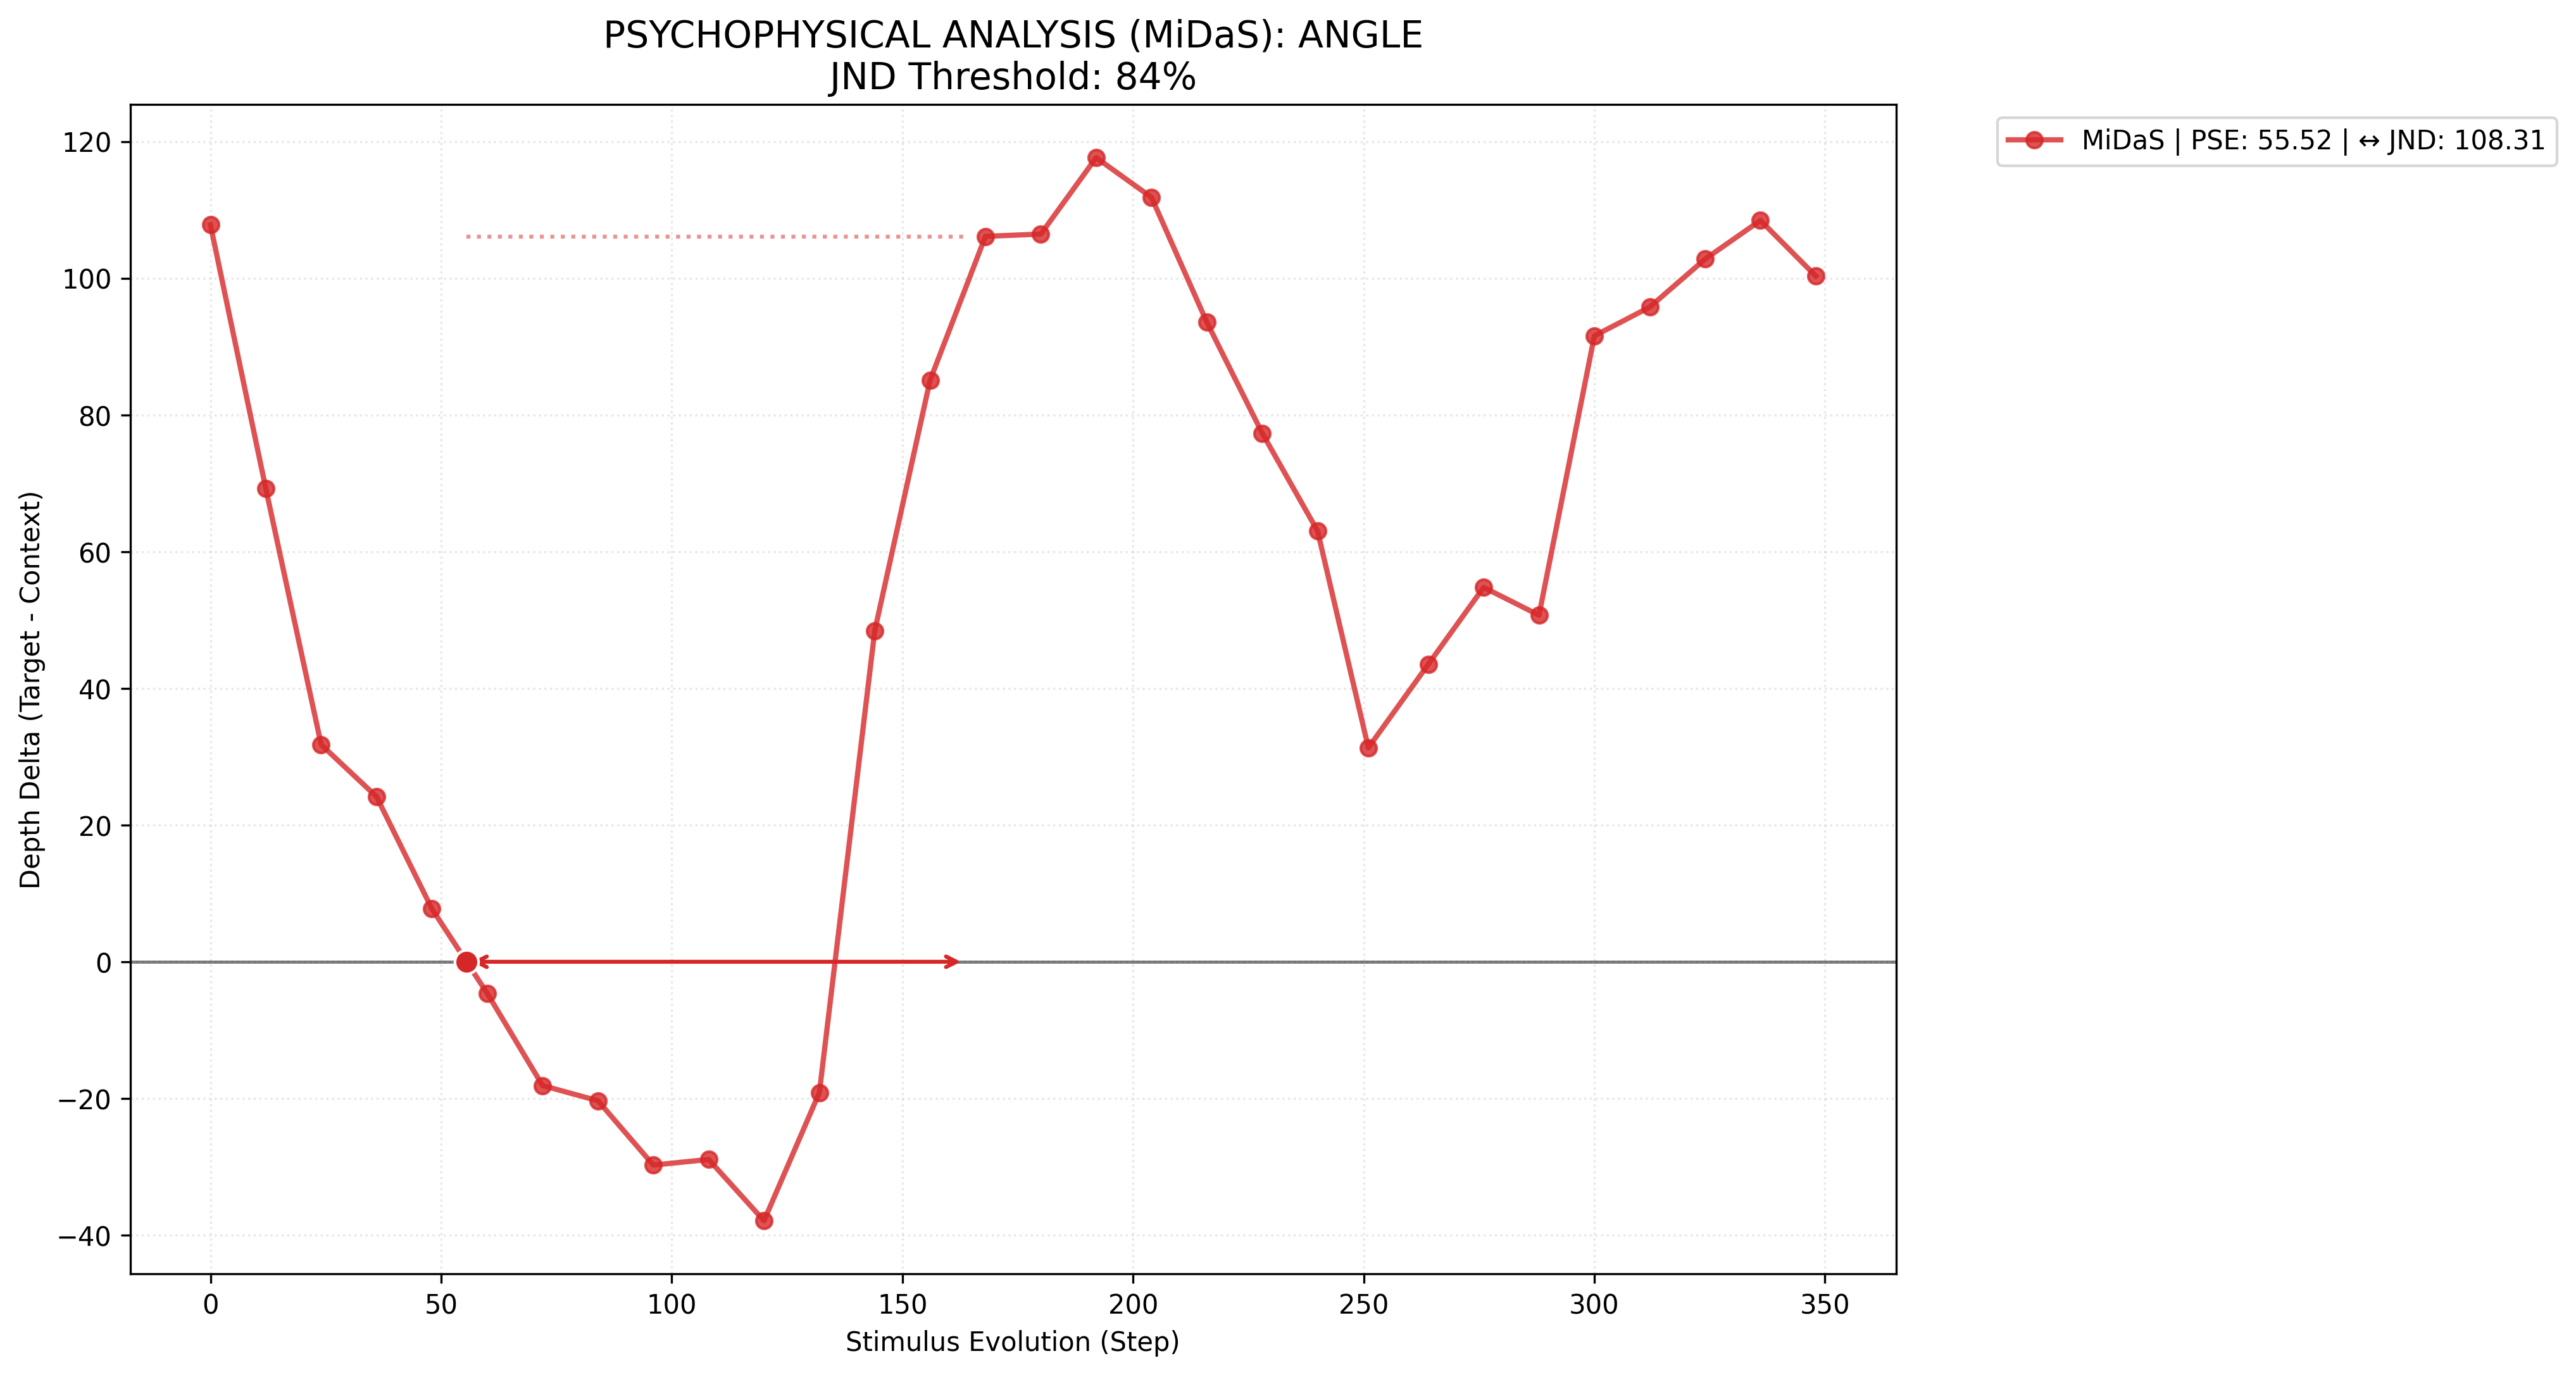
\includegraphics[width=\linewidth]{figures/fig_psy_angle.png}
        \caption{Shading Angle (High Oscillatory Volatility)}
        \label{fig:fig_psy_angle}
     \end{subfigure}
     \vspace{0.5em}
     \begin{subfigure}[b]{0.98\linewidth}
        \centering
        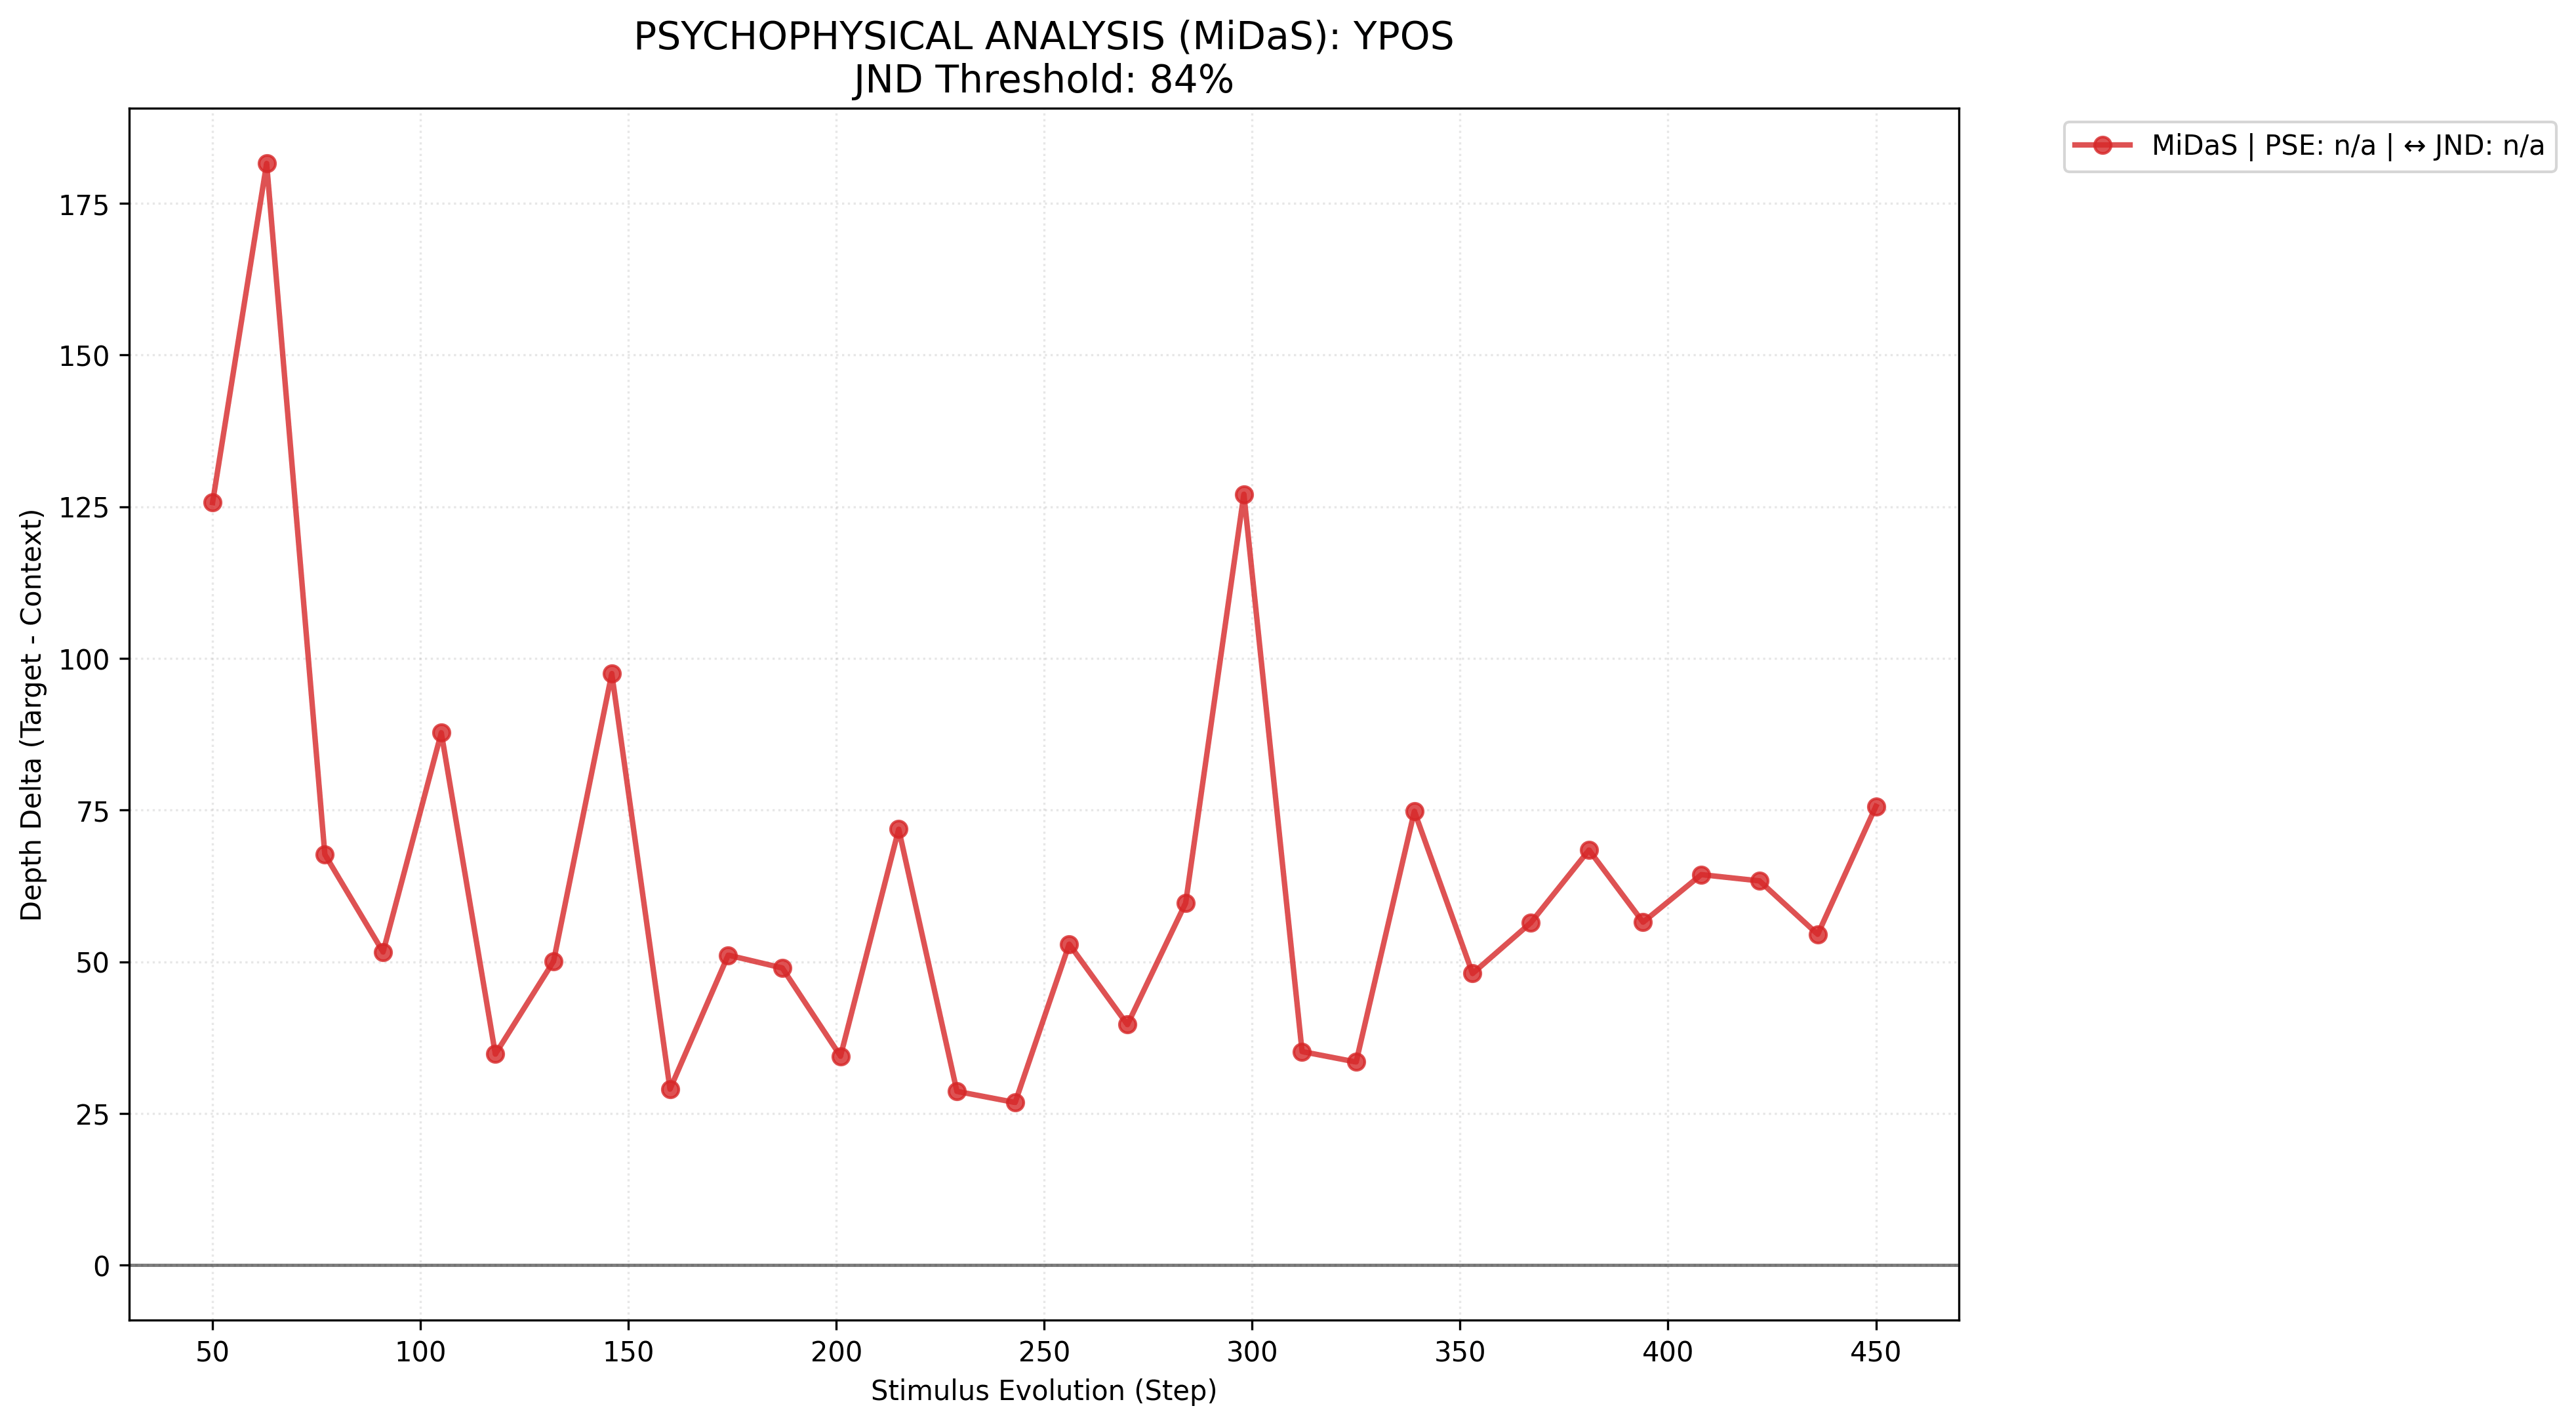
\includegraphics[width=0.52\linewidth]{figures/fig_psy_ypos.png}
        \caption{Height Bias (Rigid, Non-Crossing Trajectory)}
        \label{fig:fig_psy_ypos}
     \end{subfigure}
  \caption{Representative psychophysical response curves for MiDaS. The plots illustrate the structural variability of the CNN backbone, contrasting sharp step transitions (Ponzo) against extreme spatial volatility (Angle) and unyielding non-crossing linear trajectories (Height).}
  \label{fig:fig_midas_psychophysics}
\end{figure}
% ============================================================
\end{document}
